\documentclass[a4paper,12pt, english]{article}

\usepackage{booktabs}


\usepackage{ucs}
\usepackage[utf8]{inputenc}
\usepackage{babel}
\usepackage{fontenc}
\usepackage{graphicx}
\usepackage{a4wide}
\usepackage{etex}
% \usepackage{booktabs}
\usepackage[]{hyperref}
\usepackage{rotating}
\usepackage{bm}
\usepackage{multirow}
\usepackage{tabularx}

\usepackage{amsmath,mathptmx,amssymb}
\usepackage{bm}
\usepackage{times}
\usepackage{algorithmic}
\usepackage{todonotes}


\title{A hybrid evolutionary machine learning pipeline for longitudinal dispersion coefficient modeling}

\author{}

\date{\today}
\sloppy \hyphenpenalty 10000

\newcommand{\w}{\mathbf{w}}
\newcommand{\x}{\mathbf{x}}
\newcommand{\xp}{\bm{\theta}}

\newcommand{\xfs}{\xp^{FS}}
\newcommand{\xmb}{\xp^{MB}}


\begin{document}

\maketitle
%---------------------------------------------------------------------------------
\begin{abstract}
Among several essential indicators for river engineering sustainability, the longitudinal dispersion coefficient ($K_x$) is the main parameter present the sediment transport pollutant in natural streams. Accurate estimation of $K_x$ is highly crucial for river water quality modeling. This study is devoted on the development of ...
The $K_x$ is modeled based on several input combinations scenarios that incorporated several related physical parameters or river system. Owing to the essential configuration for the influential parameters toward the $K_x$, an evolutionary input selection approach is integrated with the proposed predictive model.     
 
\end{abstract}

%---------------------------------------------------------------------------------
\section{\label{sec:intro} Introduction}
%---------------------------------------------------------------------------------

Various types of contaminants are discharged into water bodies across the world both point and non-point forms and these contaminants adversely affects the water quality \cite{noori2007assessment}. Hence, providing an accurate pollution dispersion analysis in rivers a tedious issue for authorities responsible for monitoring and managing water resources. Even though pollution can disseminate in all directions of rivers \cite{tayfur2005predicting}, the longitudinal dispersion is normally dominant at a considerable distance from the pollution source after discharge into the water body \cite{riahi2009expert}. As per environmental and hydrological researchers, the most important parameter when studying the longitudinal transport of pollution in the rivers is the longitudinal dispersion coefficient ($K_x$) \cite{kashefipour2002longitudinal, etemad2012predicting, hamidifar2015longitudinal, dehghani2020novel, wang2017physically, farzadkhoo2018comparative, baek2019deriving, farzadkhoo2019flow}. $K_x$ accurate estimation is essential for numerous practical applications, such as environmental engineering, river engineering, intake designs, assessment of dangerous contaminants discharge into water bodies, etc. \cite{alizadeh2017improvement}. Several models exist which relies on the advection-dispersion equation (Eq. 1); however, the modelling results are highly affected by the nature of the $K_x$ \cite{noori2016reliable}.

----------- eq (1)


where $K_x$ = the longitudinal dispersion coefficient, $t$ = time, $x$ and $u$ = longitudinal coordinate and longitudinal velocity, respectively, and $C$ = averaged cross-sectional concentration \cite{noori2011framework}. Regarding $K_x$, it can be determined experimentally, empirically, and theoretically \cite{perucca2009estimation, wang2016estimating, data2019estimation, milivsic2019estimation, deng2001longitudinal, deng2002longitudinal, seo2004estimation, shin2019longitudinal, seo1998predicting, swamee2000empirical, zeng2014estimation, disley2015predictive, camacho2019quantifying}. The direct experimental determination of the dispersion coefficient demands cost and time inefficient tracer studies and could be done only with rectangular flumes data \cite{etemad2012predicting}. The determination of $K_x$ through theoretical means is also difficult as there are no knowledge of the transverse profiles of both the flow depth and flow velocity \cite{deng2001longitudinal}. The earlier predictive equations differ in their findings and are laden with certain levels of uncertainty; therefore, several studies have focused on the development of empirical models for $K_x$ estimation \cite{wang2017physically, altunkaynak2016prediction,nezaratian2018sensitivity}. Several studies have been devoted on discovering the relationship between $K_x$ and the hydrodynamic and  hydraulic parameters \cite{sahin2014empirical, tutmez2013regression,shen2010estimating} and some equations that model this relationship have been developed from these studies.

Over the past two decades, the implementation of computer aid models reported an optimistic results in modeling hydraulic engineering problems \cite{sharafati2019application}. The importance of artificial intelligence (AI) techniques in environmental modelling has increased over the years. One among several studies conducted on the $K_x$ modeling, an artificial neural network (ANN) model developed by Tayfur and Singh \cite{tayfur2005predicting} for $K_x$ prediction in rivers and natural streams. The evaluation of the model proved its capability in predicting the $K_x$ compared to the earlier suggested empirical approaches. Another study by Tayfur \cite{tayfur2006fuzzy} presented fuzzy, ANN, and regression-based models for the $K_x$ prediction in natural streams. The prediction results showed that the developed models outperformed the existing empirical equations as they are satisfactorily predicted the measured data with minimum errors.
A fuzzy model developed by Fuat Toprak and Savci \cite{fuat2007longitudinal} for $K_x$ prediction in natural channels. The study compared the performance of the developed model with measured data and the existing equations and from the results, the fuzzy model performed better than the other techniques in terms of results reliability. Toprak and Cigizoglu \cite{toprak2008predicting} applied three ANN models based on different learning algorithms (i.e., the radial basis function neural network, feed forward back propagation, and the generalized regression neural network) for $K_x$ estimation when evaluating its behavior in dispersion characteristics prediction in natural streams. The outcome of the study showed that the accuracy of the developed model was higher compared to the accuracy of the other existing empirical equations. The capacity of support vector machine (SVM) and adaptive neuro fuzzy inference system (ANFIS) models have been inspected by Noori et al. \cite{noori2009predicting} for $K_x$ prediction in natural streams. The study found that the SVM model performed better than the ANFIS model in terms of achieving better threshold statistical analysis. In another study \cite{riahi2009expert}, the authors developed ANFIS model for $K_x$ simulation in rivers and natural streams. The research finding showed satisfactory $K_x$ values prediction using the proposed model in comparison to the measured data. According to the authors conclusion, it is a good way of $K_x$ prediction in streams but can be combined with other mathematical pollutant transfer models for real-time updating of such models.

A back-propagation neural network (BPNN) model with a 2D convergent flow tracer transport model developed by Shieh et al. \cite{shieh2010development} for improved evaluation of transverse and longitudinal dispersivities from a convergent flow tracer test. From the results, the developed model required less computational time and offered more accurate values of the transport parameter. The study also found the developed method as an effective way of achieving fast and accurate transverse and longitudinal dispersivities evaluation for a field convergent flow tracer test. An ANN model presented by Sahay \cite{sahay2011prediction} for $K_x$ prediction in natural rivers. The performance of the developed model was compared with that of earlier reported models and found to be more accurate and precise. The study by Noori et al. \cite{noori2011framework}, authors employed ANN model for $K_x$ prediction in natural streams. The outcome of the study showed that the developed approach is applicable in river water quality management studies. An SVM approach constructed by Azamathulla and Wu \cite{azamathulla2011support} for $K_x$ prediction in natural rivers. The study developed the proposed model based on published data on dispersion coefficient for a range of flow conditions. Research findings showed that the developed SVM model is applicable for accurate $K_x$ prediction. A genetic programming (GP) model developed by \cite{tu2015ant} for modeling $K_x$. According to the reported studies, practicing engineers can rely on the modern data driven approaches to improve their designs and evaluations when using GP for $K_x$ prediction in natural rivers. The use of M5 model tree for $K_x$ prediction has been reported by Etemad-Shahidi and Taghipour \cite{etemad2012predicting}. The model was compared to the other existing equations in terms of performance based on error measures and from the results, the developed model performed better than the existing formulas and could be a valuable tool for $K_x$ prediction.


\textcolor{blue}{The development of an empirical formula for $K_x$ prediction in pipe flow based on the use of the evolutionary gene expression programming (GEP) has been presented by Sattar \cite{sattar2014gene}. The GEP was used for the establishment of the empirical relationships between the $K_x$ and some of the control parameters, such as the Reynolds number, the pipe friction coefficient, the average velocity, and the pipe diameter. The results showed that the proposed relations are simple and effective in $K_x$ evaluation in pipe flow. The development of an empirical formulae for $K_x$ prediction in pipe flow based on the adaptive Neuro fuzzy group method of data handling has been presented by Najafzadeh and Sattar \cite{najafzadeh2015neuro}. The evaluation of the proposed method showed that the proposed relations are simpler compared to the existing numerical solutions; it was also found as an effective way of evaluating the $K_x$ in pipe flow.}


The study by Sattar and Gharabaghi \cite{sattar2015gene} presented two GEP models for $K_x$ prediction based on 150 published data sets of hydraulic and geometric parameters in natural streams. The analysis showed that the proposed relations were accurate, simple, and effective in $K_x$ prediction in natural streams. The suitability of empirical formulas, RBF, and MLP neural network for $K_x$ prediction in rivers has been evaluated by Parsaie and Haghiabi \cite{parsaie2015predicting}. The outcome of the analysis showed that MLP performed best in $K_x$ prediction while the RBF model performed a bit better than the empirical formulas in terms of accuracy. The PSO has been introduced by Najafzadeh and Tafarojnoruz \cite{najafzadeh2016evaluation} for improving the performance of neuro-fuzzy-based group method of data handling (NF-GMDH) in $K_x$ prediction in rivers. The NF-GMDH-PSO model was compared with DE, MT, GA, ANN, and traditional empirical equations in terms of performance. From the evaluation, DE and GA methods outperformed the other among ANN-based equations. The reliability of ANN, ANFIS, and SVM in $K_x$ prediction in natural rivers has been studied by Noori et al. \cite{noori2016reliable}. The study performed forward selection (FS) and gamma test (GT) in order to sort the input variables in the order of their effects and relevance on $K_x$ prediction. The outcome of the study revealed less uncertainty in the SVM model compared to the ANN and ANFIS models for $K_x$ estimation in natural rivers; furthermore, the performance of the ANFIS model was found better than that of the ANN model. A multivariate adaptive regression splines (MARS) has been developed by Haghiabi \cite{haghiabi2016prediction} for $K_x$ prediction in rivers. The performance of the MARS model was compared to that of multi-layer neural network model and empirical formulas and the outcome showed that the MARS model performed better than the multi-layer neural network model and empirical formulas in terms of accuracy. The study by Alizadeh et al. \cite{alizadeh2017predicting} relied on the GA, imperialist competitive algorithm (ICA), bee algorithm (BA), cuckoo search (CS), and Levenberg–Marquardt (LM) algorithm for the training of ANN models for $K_x$ prediction in rivers. The evaluation of the models showed that they can be successfully used to improve the performance of ANN models. However, the performance of the CS, ICA and BA algorithms was better than that of GA and LM in training the ANN model. The use of the Bayesian network (BN) for $K_x$ prediction in natural rivers has been presented by Mohamad Javad Alizadeh et al. \cite{alizadeh2017prediction}. First, the study applied the clustering technique as a data preprocessing technique to cluster the data in separate groups of similar characteristics. The study showed that the developed model is a suitable way of pollutant transport prediction in natural rivers.

The use of evolutionary polynomial regression (EPR) for accurate prediction of Kx  in rivers has been presented by Balf et al. \cite{balf2018evolutionary}; the prediction was based on the flow depth, channel width, and average and shear velocities. The EPR model-predicted Kx was compared with those estimated using other conventional Kx  estimation formulas and from the results, the introduced EPR model for Kx estimation was found suitable to be incorporated in one-dimensional water quality models for better solute concentration prediction in natural rivers. An ANFIS-based PCA method of $K_x$ prediction has been developed by Parsaie et al.,\cite{parsaie2018anfis} . The evaluation of the model showed better accuracy of the ANFIS model compared to the experimental formulas. The study by Riahi-Madvar et al. \cite{riahi2019pareto}
 presented a Pareto-Optimal-Multigene Genetic Programming (POMGGP) equation for $K_x$ prediction kX. The study analyzed 503 data sets of channel geometry and flow conditions in natural streams in order to develop a hybrid model. The developed hybrid model is a combination of the Subset Selection of Maximum Dissimilarity Method (SSMD) with Multigene Genetic Programming (MGP) and Pareto-front optimization. The aim of the combined approach is to establish a set of selected dimensionless equations of kX and the best equation with the widest applicability. As per the authors, the proposed equation provided accurate prediction of kX compared to the other published equations; hence, it can be applied in $K_x$ prediction in natural river flows.

A hybrid approach called GRC-ANN has been presented by Ghiasi et al. \cite{ghiasi2019granular} for $K_x$ estimation in natural rivers. The hybrid method is a combination of the granular computing (GRC) method with an ANN model. The performance of the hybrid model was compared with those of ANFIS, ANN, and other empirical models in terms of accuracy and performance in different $K_x$ values. The outcome of the evaluation showed that the hybrid GRC-ANN approach performed better than the other $K_x$ prediction methods. Saberi-Movahed et al., \cite{saberi2020receiving} relied on the ELM to develop a novel group method of data handling (GMDH) called GMDH-ELM for $K_x$ prediction in water pipelines. PSO and GSA were employed to improve the feed forward structure of the GMDH-ELM model for $K_x$ prediction. The analysis of the GMDH-ELM model showed that it achieved a good level of precision in the training and testing phases. The results further showed that the proposed GMDH-ELM performed better than other soft computing and conventional predictive models.


The study by Kargar et al. \cite{kargar2020estimating} examined the performance of SVR, Gaussian process regression, random forest, M5 model tree (M5P), and MLR in $K_x$ prediction in natural streams. The study found the M5P model with simple formulations to exhibit better performance compared to the other machine learning and empirical models and was recommended as a suitable tool for $K_x$ prediction in rivers. An integrated model has been introduced by Memarzadeh et al. \cite{memarzadeh2020novel} based on the Subset Selection of Maximum Dissimilarity (SSMD) method and the Whale Optimization Algorithm (a simple optimization approach). The study presented a high accuracy formula for $K_x$ prediction which was proven to be superior in terms of $K_x$ prediction compared to the existing $K_x$ prediction formulas. The Whale optimization algorithm was also found applicable in improving the predictive performance of the equations in other related fields by establishing the optimum coefficient values. The study by Riahi-Madvar et al.\cite{riahi2020improvements} relied on the SSMD and ANFIS hybridized with the firefly algorithm (FFA) to develop a hybrid system for $K_x$ prediction. The FFA was used for the derivation of the optimum parameters of the ANFIS model. The analysis of the proposed ANFIS-FFA model showed that it was significantly improved compared to the normal ANFIS, suggesting that the parameters optimization by the nature-inspired optimization algorithms contributed significantly towards improving the generality of the ANFIS estimations.



{\color{blue}
Feature selection,  also known as variable selection or attribute selection,  is an independent process generally combined with the learning procedure of machine learning estimators, which aims to reduce the number of attributes to improve the performance of an estimator.
The central premise of feature selection is to remove from the dataset the irrelevant or redundant features, so the quality of the final predictions is not deteriorated. 

Depending on their interaction with the estimator method,
feature selection techniques can be classified into filter models,   wrapper models, and embedded models.
%
Filter models work independently of the estimator using information form the dataset relying on a metric constructed upon several statistical tests, which can be a correlation coefficient, a distance function, or an importance measure.
%
Wrapper models use an estimation model and select a subset of features based on the estimator performance. 
Although wapper methods produce better performance, they are computationally intensive and time-consuming than the filter methods \cite{tan:2020}.
%
In the embed methods,
the selection of relevant features is integrated into the learning of the estimation model \cite{cai:201870}. The selected features are those that best contribute to the accuracy of the estimation model \cite{mirzaei:2017}.
}

%Successful application of one-dimensional advection-dispersion models in rivers depends on the accuracy of the longitudinal dispersion coefficient ($K_x$)\cite{ghiasi:2020}.

%Machine learning methods are interesting alternatives to predict $K_x$ streams in natural rivers.
%Several machine learning methods are compared in \cite{katayoun:2020}.

%Recently, some hybrid approaches can be developed in the literature.
%In  \cite{ghiasi:2020}, a hybrid method combining granular computing (GRC), neural networks, and adaptive neuro-fuzzy inference system were developed for $K_x$ estimation.
%As estimation model based on the whale optimization algorithm (WOA) metaheuristic is presented in  \cite{memarzadeh:2020}.
%A comparison of various evolutionary computation optimization techniques used to train neural networks for estimating of longitudinal dispersion coefficient in rivers in presented in \cite{piotrowski:2012}.

%---------------------------------------------------------------------------------
\section{\label{sec:methods} Materials and Methods}
%---------------------------------------------------------------------------------

%---------------------------------------------------------------------------------
\subsection{\label{sec:methods:dataset} Longitudinal Dispersion Data}
%---------------------------------------------------------------------------------
The dataset available in \cite{tayfur2005predicting} consists of 71 samples of hydromorphological parameters and longitudinal dispersion coefficients obtained from 29 rivers on the United States.  
From this dataset, fifty-one samples (72\%) are used to compose the training set, while the remaining 20 samples (28\%) comprise the test set. Table \ref{tab:input-output-var} presents a short description of the variables and also displays the statistical information of the variables in the dataset.
%
The relative shear velocity, also known as friction term,
 can be associated with as the
roughnesses and hydrodynamic characteristics of the river bed \cite{etemad2012predicting}.
The shape channel shape parameter, given by  $\beta=\ln{(B/H)}$,  reflects  the vertical
 irregularities of the river bed \cite{deng2001longitudinal}.
The channel sinuosity is defined as the ratio of the channel length to the valley length \cite{sahay:2013}. 
% 
\begin{table}[!htb]
\centering
\caption{ \label{tab:input-output-var} Statistical information  of the dataset and short description of he variables. }
\begin{center}
\begin{tabular}{clrrrr}
 \hline
Variable           &     Short description                     &   min&   mean &    std &     max \\ \hline
$ B     $ (m)      &     channel width                         & 11.90&  82.96 & 122.50 & 711.20  \\
$ H     $ (m)      &     cross-sectional average flow depth    &  0.22&   1.71 &   2.60 &  19.94  \\
$ U     $ (m/s)    &     cross-sectional average flow velocity & 0.034&   0.54 &   0.39 &   1.74  \\
$ u^*   $ (m/s)    &     shear velocity                        & 0.002&  0.088 &  0.089 &  0.553  \\
$ U/u^* $          &     relative shear velocity               & 13.80&  51.68 &  31.72 & 156.50  \\
$ Q     $ (m$^3$/s)&     flow discharge                        &  1.29&   7.62 &   4.56 &  19.63  \\
$ \beta $          &     channel shape parameter               &  2.62&   3.79 &   0.57 &   5.05  \\
$ \sigma$          &     channel sinuosity                     &  1.08&   1.51 &   0.42 &   2.54  \\\hline
$ K_x   $ (m$^2$/s)&     longitudinal dispersion coefficient   &  1.90& 107.71 & 170.25 & 892.00  \\ \hline
\end{tabular}
\end{center}
\end{table}

%---------------------------------------------------------------------------------
\subsection{\label{sec:methods:evofs} Proposed Hybrid Method}
%---------------------------------------------------------------------------------

The focus of this work is developing a machine learning pipeline for the prediction of the dispersion coefficient of natural channels. 
A machine learning pipeline comprises a set of chained steps that involves processing the data, select the features, build the machine learning estimator, and finally releasing final model to predict the outputs.
Also, machine learning pipelines reduce the human effort when building a reliable and accurate model \cite{liu:201748}.

Figure \ref{fig:framework} depicts the machine learning pipeline proposed in this paper.
The pipeline consists of three steps: data processing, feature selection, and model building.
% 
In the the data processing step, the samples in the data set are scaled according to
\[
 v_i = \frac{v_i}{v_{max}}, \quad
 v_i \in \{ {B}, {H}, {Q}, {U}, {u^*}, {U/u^*}, {\beta}, {\sigma}, \}
\]
where $v_i$ is the standardized value, and $v_{max}$  is the maximum values for the samples of the considered variable. 

\begin{figure}[!htb]
 \centering 
 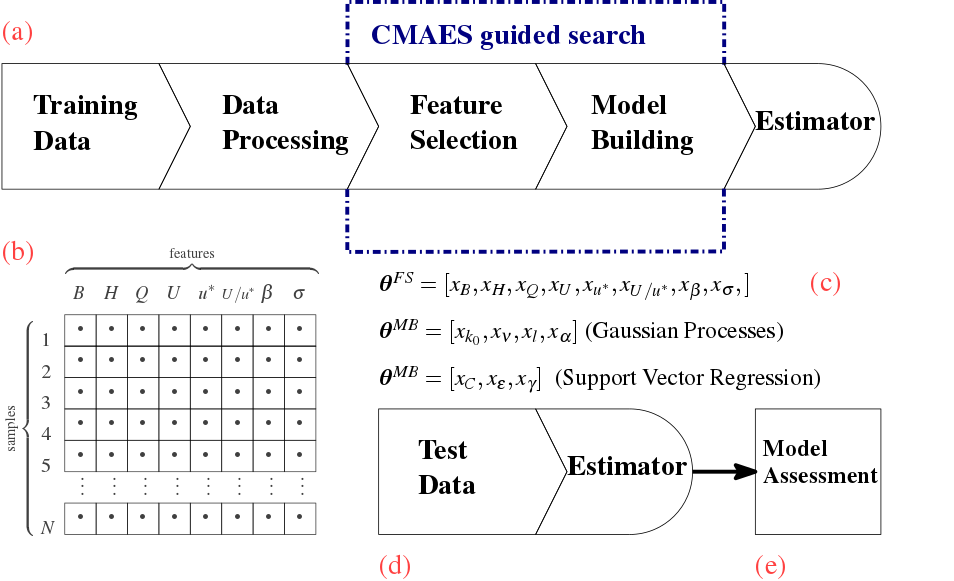
\includegraphics[width=0.85\linewidth]{./framework/ldc_model_scheme}
 \caption{Proposed hybrid framework}
 \label{fig:framework}
\end{figure}

A simple procedure is used in the feature selection step. A feature vector, composed by 8 entries
\[ \xfs = [ x_{B}, x_{H}, x_{Q}, x_{U}, x_{u^*}, x_{U/u^*}, x_{\beta}, x_{\sigma}]\]
represent the eight variables in Table \ref{tab:input-output-var}.
An  entry equals to 1 represent a selected feature and 0 a removed feature. For example, the feature vector $ \xfs = [10100011] $ means that the selected set $\{B, Q, \beta, \sigma \}$ is used to produce the $K_x$ predictions.

The third step implements the model building procedure, that receives the features selected in the previous step and use them to train the machine learning model.
Two machine learning were used along with the pipeline: Gaussian Regression Regression (GPR) and Support Vector Regression (SVR).

%%---------------------------------------------------------------------------------
%\subsection{\label{sec:methods:gpr} Gaussian Processes Regression}
%%---------------------------------------------------------------------------------
{\color{red}
In Gaussian process regression (GPR), it is assumed the output $\hat{y}$ of a function  $f(\x)$ can be written as 
\[
 \hat{y} = f(\x) + \varepsilon
\]
with the noise term is considered as $\varepsilon \sim N(0, \sigma^2)$. The predictive distribution of the output variable $\hat{y}$, given its input $\x$, is \cite{wang2015159}
\[
 \hat{y} = \mathbf{k}^T(\x) \mathbf{C}^{-1}\mathbf{y},
\]
where 
$\mathbf{y}$ is the vector of training data, 
$\mathbf{k} = [ C(\x, \x_1, \dots, C(\x, \x_N) ]^T$, and $\mathbf{C}$ is the covariance matrix function.
The covariance function   models the dependence between the function values at different input points  $\x_i$ and $\x_j$ \cite{schulz:20181}:
\[
\mathbf{C}(\x_i, \x_j) = \mathbf{K}(\x_i, \x_j) + \gamma \mathbf{I}
\]
where 
\begin{equation}
 \label{eq:gpr-kernel-matern}
  K_{ij} = K(\x_i, \x_j) = 
  k_0 \frac{2^{1-\nu}}{\Gamma(\nu)}  
 \left( ||(\x_i, \x_j)|| \sqrt{\frac{2\nu}{l}} \right)^{\nu} 
 K_{\nu}\left( ||(\x_i, \x_j)|| \sqrt{\frac{2\nu}{l} } \right)
\end{equation}
where $\nu$ and $l$ are positive parameters, $\Gamma$ is the Gamma function and $ K_{\nu}$ is the modified Bessel function \cite{kumar:2020101986}.

The building of the GPR model involves the proper setting of the kernel parameters
${k_0}, {\nu}$, and  ${l}$ and the regularization coefficient ${\alpha}$.
The model building vector for GPR machine learning model is represented by
$\xmb = [ {k_0}, {\nu}, {l}, {\alpha} ]$.
}

%%----------------------------------------------------------------------------------
%\subsubsection{ Support Vector Regression -- SVR}
%%----------------------------------------------------------------------------------
The Support Vector Regression (SVR)  builds a linear regression model of the form
\[
f(\x) = \sum_{j=1}^{N} w_j K(\x,\x_j) + b\]
where $K(\cdot, \cdot) $ is a nonlinear transformation, $\w = [w_1, \cdots, w_N]$, is the vector of weights, $b$ is  a constant threshold and $N$ is the number os samples.
The  nonlinear transformation used in this paper is the radial basis kernel function of the form 
\begin{equation}
 \label{eq:svr-kernel}
K(\x,\x_i) = \sum_{i=1}^{N} \exp(-\gamma \|\x-\x_i\|^2) )
\end{equation}
% 
where $\gamma$ is the bandwidth parameter.

In SVR the optimal $\w$ and $b$ are computed by minimizing the functional \cite{katayoun:2020}
\[
J = \sum_{i=1}^{N} w_i^2 +  \frac{1}{N} \sum_{i=1}^{N} L_{\varepsilon} ( y_i - f(\x_i) ), \quad
L_{\varepsilon}(y - f(\x))=
\begin{cases}
  0           \mbox{ if } |y - f(\x)|\le \varepsilon\\
  |y - f(\x)|  \mbox{ otherwise }
\end{cases}
\]
where 
$y_i$ is output data associated with $\x_i$, $ L_{\varepsilon}$ is the $\varepsilon$-insensitive loss function \cite{gunn:1998} and $\varepsilon$ is a SVR parameter. 
The internal parameters of the SRV model to be adjusted are $C, \varepsilon$ and $\gamma$, resulting the the model building parameter $\xmb = [ {C}, {\epsilon}, {\gamma}]$.


The parameterization of the pipeline comprises the adjustment of two vectors  $\xfs$ and $\xmb$. These two vectors are then concatenated in a parametric vector
\[ \xp = [ \xfs,  \xmb ] \]
where $\xfs$ is the feature vector and  $\xmb$ is the vector of the internal parameters of the machine learning method.
 
%%---------------------------------------------------------------------------------
%\subsection{\label{sec:methods:cmaes} Covariance Matrix Evolution Strategies}
%%---------------------------------------------------------------------------------

As shown proposed in the framework shown in Figure \ref{fig:framework}, an evolution strategy assists the feature selection and the adjustment of the internal parameters of the machine learning model.  
The pipeline representation for a solution implementing the Gaussian Process machine learning is represented by 12-dimensional vector
$$\xp = [ x_{B}, x_{H}, x_{Q}, x_{U}, x_{u^*}, x_{U/u^*}, x_{\beta}, x_{\sigma}, {k_0}, {\nu}, {l}, {\alpha} ]$$
while the the 11-dimensional parametric vector 
$$\xp = [ x_{B}, x_{H}, x_{Q}, x_{U}, x_{u^*}, x_{U/u^*}, x_{\beta}, x_{\sigma}, {C}, {\epsilon}, {\gamma}] $$
encodes a  solution implementing a Support Vector machine machine learning model.

The hybrid pipeline implements the Covariance Matrix Adaptation Evolution Strategy (CMAES), a variant of the evolution strategy algorithm \cite{hansen:2001}. CMAES performs the optimization by iteratively sampling candidate solutions from a multidimensional normal distribution based on a vector  of means $m$, a  $n \times n$ covariance matrix $C$ using a step size $\sigma$ \cite{beyer:2002}. 
{\color{red}
During the search, the CMAES minimizes the objective function given by the 
the Root Mean Discrepancy averaged over all $N$ observations 
\begin{equation}
 \label{eq:rmdr}
 \mbox{RMD} = \frac{1}{N} \sum_{i=1}^{N} \left( \log{ \frac{K_{xp_i}}{K_{xm_i}} } \right)^2 
\end{equation} 
% 
where $K_{xp_i}$ and $K_{xm_i}$ are the prediction and observed dispersions.
}
The pseudocode of CMAES is presented in Figure \ref{fig:algo_cmaes}. A detailed explanation of the CMAES algorithm and the parameters can be found in \cite{Li:2018}.

\begin{figure}[!htb]
\begin{algorithmic}[1]
% \STATE set $\lambda$
\STATE initialize $m_0=0, \sigma_0=0.5, C_0=I, p_0=0, s_0=0, k=0, \mu=\lambda/2$ \label{lin:init-0}
\STATE initialize $\{ (\xp_i, z_i=OF(\xp_i)), i=1, \dots, \lambda \}$ \label{lin:init-1}
\WHILE {$k <  N_G$} 
    \FOR{$i=1$ to $\lambda$} 
        \STATE $\xp_i = m_k + \sigma_k \mathcal  {N}(0, C_k)$ \label{lin:sample-1}
        \STATE $f_i = OF(\xp_i)$ \label{lin:sample-2} %\COMMENT{Evaluate candidate solutions}
    \ENDFOR 
    \STATE sort solutions $\xp_{{1...\lambda }} \gets \xp_{{s(1)...s(\lambda )}}$ with $s(i) = {\mathrm{argsort}_{f}}
(f_{{1...\lambda }},  i) $ \label{lin:sort-1}
    %\STATE set  $w_{1:\mu} = \{ w_{1} \geq w_{2}\geq \dots \geq w_{\mu }>0 | \sum_{i=1}^{\mu} w_i = 1\}$    
    \STATE $m_{k+1} = m_k + \sum_{i=1}^{\mu} w_i (\xp_{1:\lambda} - m_k) $ \label{lin:mean-2}
    \STATE $s_{k+1} = (1-c_{\sigma})s_k + \sqrt{\mu_{eff}}\sqrt{c_{\sigma}(2-c_{\sigma})} C_{k}^{-1/2}\frac{m_{k+1}-m_k}{\sigma_k} $ \label{lin:path-1}
    \STATE $p_{k+1} = (1-c_c)p_k + h_{\sigma}\sqrt{\mu_{eff}}\sqrt{c_c(2-c_c)}  \frac{m_{k+1}-m_k}{\sigma_k}$ \label{lin:path-2}
    \STATE $C_{k+1} = (1-c_1-c_{\mu})C_k + c_1p_{k+1}p_{k+1}^T 
%  + (1 - h_{\sigma})c_c (2 - c_c)C_k
 +\frac{c_{\mu}}{\sigma_k^2} \sum_{i=1}^{\mu}  w_i (\xp_{1:\lambda} - m_k)w_i (\xp_{1:\lambda} - m_k)^T$ \label{lin:adapt-1}
    \STATE $\sigma_{k+1} = \sigma_k \exp{\left[ \frac{c_{\sigma}}{d_{\sigma}} \left( \frac{\|s_{k+1}\|}{ \chi_n } - 1 \right) \right]} $ \label{lin:adapt-2}
    \STATE $k\gets k+1$
\ENDWHILE 
\end{algorithmic}
\caption{\label{fig:algo_cmaes} 
Pseudocode of the Evolution Strategy algorithm to perform the feature selection and the adjustment of the internal parameters of the machine learning model.
}
\end{figure}


After the simultaneous optimization of the feature and model building vectors, the estimator is ready to be used as a $k_x$ estimator in the test set.
\todo{describe here the model assesment and metrics}


%The Discrepancy Ratio DR is used as error measure in the literature and, for each sample, it is written as
%\begin{equation}
% \label{eq:drc}
% \mbox{DR} = \log{ \frac{K_{xp}}{K_{xm}} }
%\end{equation}
%%
%where
%$K_{xm}$ is measured dispersion coefficient, and 
%$K_{xp}$ is predicted dispersion coefficient. 
%When $K_{xp}=K_{xm}$, DR is equals to zero and there is an exact prediction. Otherwise,  there is either an overprediction when $\mbox{DR}> 0$, that means  $K_{xp}>K_{xm}$, or an underprediction which leads to $\mbox{DR} < 0$ and consequently  $K_{xp}<K_{xm}$. 

%The Root Mean Discrepancy is averaged over all $N$ number of observations 
%\begin{equation}
% \label{eq:rmdr}
% \mbox{RMDR} = \frac{1}{N} \sum_{i=1}^{N} \left( \log{ \frac{K_{xp_i}}{K_{xm_i}} } \right)^2 
%\end{equation} 
%% 
%where $K_{xp_i}$ and $K_{xm_i}$ are the prediction and observed dispersions.

%%---------------------------------------------------------------------------------
%\subsection{\label{sec:methods:evofs} Feature Selection Approach}
%%---------------------------------------------------------------------------------


%---------------------------------------------------------------------------------
\section{\label{sec:results} Computational Experiments and Discussion}
%---------------------------------------------------------------------------------

The machine learning pipeline proposed in this paper was applied to predicting the coefficient of longitudinal dispersion, and their performance was compared with the models proposed in \cite{tayfur2005predicting}. 
% 
A robust procedure was proposed to report the results: (1) perform 100 independent runs establishing a unique random seed for each run; (2) for each run, the hybrid pipeline models built on the training set are used to estimate the dispersion coefficients in the test set;  (3) calculate the metrics RMSE and Accuracy to asses the performance of each model.
%The selected features in the first step of the experiments are summarized in Table \ref{tab:cases-features}.

\begin{table}[!htb]
    \centering
    \caption{ \label{tab:cases-features} Input features associated with models tested in this paper.
    Case 0 involves eight input variables while Cases 1-7 were proposed by \cite{tayfur2005predicting}.
    }
    \begin{tabular}{ccl}
    \hline
      Case   & $\xfs$ (fixed mask) & Active features                         \\ \hline
      Case 0 &  11111111   & $U , H , B, u^*, Q, U/u^*, \beta,\sigma$\\ 
      Case 1 &  11100000   & $U , H , B                             $\\
      Case 2 &  00001000   & $Q                                     $\\
      Case 3 &  10000000   & $U                                     $\\
      Case 4 &  10000010   & $U, \beta                              $\\
      Case 5 &  10000011   & $U, \beta, \sigma                      $\\
      Case 6 &  00000100   & $U/u^*                                 $\\
      Case 7 &  00000111   & $U/u^*, \beta, \sigma                  $\\ \hline
    \end{tabular}
\end{table}


The computational experiments were divided into three parts:
\begin{enumerate}

\item Modeling $K_x$ without feature selection. 
 Perform experiments using the machine learning approach proposed considering all features (Case 0) and also reproduce the models presented in \cite{tayfur2005predicting} (Cases 1-7) shown in Table \ref{tab:cases-features}. 
 For these experiments, the vector $\xfs$ is kept constant, depending on the $K_x$ model. 
 %Table \ref{tab:cases-features} shows all models ant the respective $\xfs$ vector associated with the model. 
 In this experiment, only the machine learning parametric vector $\xmb$ is adjusted to fine-tunning the machine learning model.
 
 \item Modeling $K_x$ using evolutionary feature selection. 
 Employ the hybrid pipeline shown in Figure \ref{fig:framework} to simultaneously search for the most suitable feature set and the model parameters. The feature selection allows for exploring combinations of features that are not presented in Table \ref{tab:cases-features}, and that can potentially produce better results when used as inputs for GPR and SVR. 
 
 \item Modeling $K_x$ with the most frequent features. 
 Build machine learning models using the most frequent features found in the previous experiment, exploiting the previous knowledge on the features and model parameters to propose an accurate model.
 
\end{enumerate}


% A feedforward artificial neural network was constructed to model LDC in \cite{tayfur2005predicting}. 
% The number of layers and the number of neurons in each layer were found using a trial-and-error procedure.
Considering the Table  \ref{tab:cases-features}, 
Case 0  employs the original features to model the dispersion coefficient of natural streams.
% Cases 1-7 follows the description in \cite{tayfur2005predicting}.
Cases 1-7 were proposed in \cite{tayfur2005predicting}, where a neural network was used to to predict $K_x$.
Case 1  considers three features involving flow and geometric characteristics: the flow velocity $U$, the flow depth $H$, and the channel width $B$.
Case 2 employs only flow discharge $Q$ as the input feature.
As the velocity plays an important role in the forecast of the effects of a pollutant spill, Case 3  considered only flow velocity $U$.
Case 4 considered flow velocity $U$ and channel shape parameter $\beta$ as input variables, while Case 5 considered channel sinuosity $\sigma$ in the feature vector $\xfs$ along with the channel shape parameter $\beta$ and flow velocity $U$.
Case 6 considered only the relative shear velocity $U/u^*$.
Finally, Case 7 considered the channel shaper parameter $\beta$ and channel sinuosity $\sigma$ along with the relative shear velocity $U/u*$ as input features.

% % \rotatebox{90}{
% \begin{table}[htp]
% % \begin{sidewaystable}[!tbp]
%  \centering
%  \caption{\label{tab:sum-results} 
%  To be inserted
%  }
% \begin{table}
\centering
\caption{Caption to be inserted.}
\label{eml_____comparison_datasets_table}
\begin{tabular}{rrrrrr}
\toprule
Dataset & Estimator &       RMSE$(K_x<100)$ &         RMSE$(B/H<50)$ &                   RMSE &             Accuracy \\
\midrule
 Case 0 &       GPR &          33.33 (4.41) &          78.99 (85.37) &         118.48 (89.18) &         65.75 (6.14) \\
 Case 0 &    GPR-FS &          32.95 (4.50) &          63.05 (15.49) &          96.77 (28.21) &  { \bf 71.60} (7.93) \\
 Case 0 &       REF &     { \bf 19.30} (--) &            183.00 (--) &            193.00 (--) &           70.00 (--) \\
 Case 0 &       SVR &          44.49 (4.44) &           64.63 (8.17) &         118.42 (25.70) &         55.65 (7.27) \\
 Case 0 &    SVR-FS &          40.75 (8.98) &    { \bf 49.91} (9.19) &   { \bf 96.48} (16.50) &        64.05 (10.43) \\
 Case 1 &       GPR &          46.01 (8.94) &        133.93 (108.09) &        175.07 (115.62) &         64.70 (7.38) \\
 Case 1 &       REF &     { \bf 21.20} (--) &            183.00 (--) &            193.00 (--) &    { \bf 75.00} (--) \\
 Case 1 &       SVR &          47.71 (8.43) &   { \bf 69.43} (16.23) &  { \bf 119.10} (33.97) &         58.50 (7.09) \\
 Case 2 &       GPR &          32.47 (9.81) &    { \bf 64.35} (2.55) &          230.80 (4.35) &         42.85 (7.66) \\
 Case 2 &       REF &     { \bf 20.00} (--) &            179.00 (--) &     { \bf 191.00} (--) &    { \bf 65.00} (--) \\
 Case 2 &       SVR &          30.27 (3.77) &           67.26 (0.94) &          233.93 (1.43) &         37.20 (5.26) \\
 Case 3 &       GPR &        150.40 (23.67) &         169.03 (23.89) &         179.73 (26.42) &         47.55 (3.71) \\
 Case 3 &       REF &           146.00 (--) &            164.00 (--) &            170.00 (--) &           40.00 (--) \\
 Case 3 &       SVR &  { \bf 86.63} (14.92) &  { \bf 109.95} (14.00) &  { \bf 168.04} (15.21) &  { \bf 53.15} (4.45) \\
 Case 4 &       GPR &         112.92 (5.16) &          120.60 (7.32) &         145.77 (15.39) &         51.60 (7.00) \\
 Case 4 &       REF &           105.00 (--) &            118.00 (--) &     { \bf 137.00} (--) &    { \bf 70.00} (--) \\
 Case 4 &       SVR &  { \bf 78.90} (14.05) &   { \bf 99.47} (13.11) &         159.58 (23.14) &         61.40 (5.48) \\
 Case 5 &       GPR &         86.39 (10.86) &          92.50 (12.50) &         124.29 (13.04) &         57.15 (5.67) \\
 Case 5 &       REF &            77.70 (--) &             99.00 (--) &     { \bf 119.00} (--) &    { \bf 58.00} (--) \\
 Case 5 &       SVR &  { \bf 61.38} (15.63) &   { \bf 83.26} (12.20) &         145.16 (18.66) &         52.20 (5.84) \\
 Case 6 &       GPR &         33.84 (14.36) &           57.47 (7.73) &         222.06 (19.19) &         44.80 (2.11) \\
 Case 6 &       REF &           104.30 (--) &      { \bf 42.00} (--) &     { \bf 159.00} (--) &    { \bf 50.00} (--) \\
 Case 6 &       SVR &   { \bf 26.30} (6.53) &           56.10 (6.27) &         217.73 (14.21) &         46.00 (3.39) \\
 Case 7 &       GPR &         57.26 (28.38) &   { \bf 53.19} (12.34) &         196.70 (33.48) &         48.10 (5.28) \\
 Case 7 &       REF &            93.80 (--) &             67.00 (--) &     { \bf 142.00} (--) &    { \bf 58.00} (--) \\
 Case 7 &       SVR &   { \bf 30.93} (6.68) &           59.55 (4.32) &          216.74 (9.67) &         35.35 (5.30) \\
 Case 8 &       GPR &   { \bf 31.36} (5.67) &          62.98 (27.28) &   { \bf 91.86} (31.55) &  { \bf 75.55} (6.82) \\
 Case 8 &       SVR &          33.21 (6.44) &   { \bf 52.49} (15.33) &         117.77 (27.33) &         68.90 (8.79) \\
\bottomrule
\end{tabular}
\end{table}

% % \end{sidewaystable} 
% \end{table}
% % }

% %---------------------------------------------------------------------------------
% \subsection{\label{sec:sub:hyb-results} Hybrid model results}
% %---------------------------------------------------------------------------------


%---------------------------------------------------------------------------------
\subsection{\label{sec:ldc-nfs} Modeling $K_x$ without feature selection }
%---------------------------------------------------------------------------------

% \begin{table}
\centering
\caption{Caption to be inserted.}
\label{eml_____comparison_datasets_table}
{\small
\begin{tabular}{rrrrrr}
\hline
 Case   &     Model &                   RMSE &            Accuracy &       RMSE$(K_x<100)$ &         RMSE$(B/H<50)$ \\
\hline
 Case 0 &       GPR &   { \bf 99.70} (29.05) &         67.91 (5.05)&          31.80 (3.97) &          63.13 (10.63)  \\
        &       SVR &         112.34 (26.40) &         57.73 (7.06)&          41.23 (4.28) &    { \bf 58.80} (7.58)  \\
        &       REF &            193.00 (--) &    { \bf 70.00} (--)&     { \bf 19.30} (--) &            183.00 (--)  \\\\
 Case 1 &       GPR &        167.34 (115.45) &         71.05 (6.19)&          41.28 (8.16) &         114.68 (98.36)  \\
        &       SVR &  { \bf 113.22} (35.35) &         62.59 (5.96)&          45.18 (8.84) &   { \bf 61.73} (14.43)  \\
        &       REF &            193.00 (--) &    { \bf 75.00} (--)&     { \bf 21.20} (--) &            183.00 (--)  \\\\
 Case 2 &       GPR &          220.19 (4.75) &         38.95 (8.29)&         34.24 (11.68) &    { \bf 61.71} (4.11)  \\
        &       SVR &          223.16 (1.37) &         39.68 (4.80)&          28.80 (3.79) &           61.80 (0.98)  \\
        &       REF &     { \bf 191.00} (--) &    { \bf 65.00} (--)&     { \bf 20.00} (--) &            179.00 (--)  \\\\
 Case 3 &       GPR &         173.80 (29.75) &         44.59 (3.19)&        143.50 (26.19) &         157.58 (25.73)  \\
        &       SVR &  { \bf 161.17} (14.32) &  { \bf 57.59} (4.12)&  { \bf 81.01} (13.24) &  { \bf 100.34} (12.62)  \\
        &       REF &            170.00 (--) &           40.00 (--)&           146.00 (--) &            164.00 (--)  \\\\
 Case 4 &       GPR &         140.90 (10.30) &         50.59 (6.51)&         106.84 (4.39) &          112.15 (6.03)  \\
        &       SVR &         150.71 (22.14) &         65.45 (5.18)&  { \bf 74.19} (12.28) &   { \bf 91.45} (11.13)  \\
        &       REF &     { \bf 137.00} (--) &    { \bf 70.00} (--)&           105.00 (--) &            118.00 (--)  \\\\
 Case 5 &       GPR &         120.54 (17.04) &         57.23 (5.64)&         82.52 (12.04) &          86.78 (13.88)  \\
        &       SVR &         138.71 (15.85) &         52.73 (3.75)&   { \bf 57.44} (9.30) &    { \bf 77.28} (7.13)  \\
        &       REF &     { \bf 119.00} (--) &    { \bf 58.00} (--)&            77.70 (--) &             99.00 (--)  \\\\
 Case 6 &       GPR &         207.78 (21.96) &         40.45 (2.91)&         43.51 (24.94) &           58.80 (2.31)  \\
        &       SVR &         203.51 (11.57) &         41.36 (3.12)&   { \bf 31.55} (9.48) &           52.82 (5.75)  \\
        &       REF &     { \bf 159.00} (--) &    { \bf 50.00} (--)&           104.30 (--) &      { \bf 42.00} (--)  \\\\
 Case 7 &       GPR &         178.87 (24.92) &         43.23 (5.77)&        101.43 (41.13) &          81.42 (18.61)  \\
        &       SVR &          203.44 (7.64) &         33.45 (3.78)&   { \bf 38.60} (9.93) &    { \bf 58.60} (6.11)  \\
        &       REF &     { \bf 142.00} (--) &    { \bf 58.00} (--)&            93.80 (--) &             67.00 (--)  \\
\hline
\end{tabular}
}
\end{table}

% RMSE$($K_x<100$)$
% RMSE$(B/H<50)$

% \begin{table}
\centering
\caption{Caption to be inserted.}
\label{eml_____comparison_datasets_table}
\begin{tabular}{rrrrrr}
\toprule
Dataset & Estimator &       RMSE$(K_x<100)$ &         RMSE$(B/H<50)$ &                   RMSE &             Accuracy \\
\midrule
 Case 0 &       GPR &          33.33 (4.41) &          78.99 (85.37) &         118.48 (89.18) &         65.75 (6.14) \\
 Case 0 &    GPR-FS &          32.95 (4.50) &          63.05 (15.49) &          96.77 (28.21) &  { \bf 71.60} (7.93) \\
 Case 0 &       REF &     { \bf 19.30} (--) &            183.00 (--) &            193.00 (--) &           70.00 (--) \\
 Case 0 &       SVR &          44.49 (4.44) &           64.63 (8.17) &         118.42 (25.70) &         55.65 (7.27) \\
 Case 0 &    SVR-FS &          40.75 (8.98) &    { \bf 49.91} (9.19) &   { \bf 96.48} (16.50) &        64.05 (10.43) \\
 Case 1 &       GPR &          46.01 (8.94) &        133.93 (108.09) &        175.07 (115.62) &         64.70 (7.38) \\
 Case 1 &       REF &     { \bf 21.20} (--) &            183.00 (--) &            193.00 (--) &    { \bf 75.00} (--) \\
 Case 1 &       SVR &          47.71 (8.43) &   { \bf 69.43} (16.23) &  { \bf 119.10} (33.97) &         58.50 (7.09) \\
 Case 2 &       GPR &          32.47 (9.81) &    { \bf 64.35} (2.55) &          230.80 (4.35) &         42.85 (7.66) \\
 Case 2 &       REF &     { \bf 20.00} (--) &            179.00 (--) &     { \bf 191.00} (--) &    { \bf 65.00} (--) \\
 Case 2 &       SVR &          30.27 (3.77) &           67.26 (0.94) &          233.93 (1.43) &         37.20 (5.26) \\
 Case 3 &       GPR &        150.40 (23.67) &         169.03 (23.89) &         179.73 (26.42) &         47.55 (3.71) \\
 Case 3 &       REF &           146.00 (--) &            164.00 (--) &            170.00 (--) &           40.00 (--) \\
 Case 3 &       SVR &  { \bf 86.63} (14.92) &  { \bf 109.95} (14.00) &  { \bf 168.04} (15.21) &  { \bf 53.15} (4.45) \\
 Case 4 &       GPR &         112.92 (5.16) &          120.60 (7.32) &         145.77 (15.39) &         51.60 (7.00) \\
 Case 4 &       REF &           105.00 (--) &            118.00 (--) &     { \bf 137.00} (--) &    { \bf 70.00} (--) \\
 Case 4 &       SVR &  { \bf 78.90} (14.05) &   { \bf 99.47} (13.11) &         159.58 (23.14) &         61.40 (5.48) \\
 Case 5 &       GPR &         86.39 (10.86) &          92.50 (12.50) &         124.29 (13.04) &         57.15 (5.67) \\
 Case 5 &       REF &            77.70 (--) &             99.00 (--) &     { \bf 119.00} (--) &    { \bf 58.00} (--) \\
 Case 5 &       SVR &  { \bf 61.38} (15.63) &   { \bf 83.26} (12.20) &         145.16 (18.66) &         52.20 (5.84) \\
 Case 6 &       GPR &         33.84 (14.36) &           57.47 (7.73) &         222.06 (19.19) &         44.80 (2.11) \\
 Case 6 &       REF &           104.30 (--) &      { \bf 42.00} (--) &     { \bf 159.00} (--) &    { \bf 50.00} (--) \\
 Case 6 &       SVR &   { \bf 26.30} (6.53) &           56.10 (6.27) &         217.73 (14.21) &         46.00 (3.39) \\
 Case 7 &       GPR &         57.26 (28.38) &   { \bf 53.19} (12.34) &         196.70 (33.48) &         48.10 (5.28) \\
 Case 7 &       REF &            93.80 (--) &             67.00 (--) &     { \bf 142.00} (--) &    { \bf 58.00} (--) \\
 Case 7 &       SVR &   { \bf 30.93} (6.68) &           59.55 (4.32) &          216.74 (9.67) &         35.35 (5.30) \\
 Case 8 &       GPR &   { \bf 31.36} (5.67) &          62.98 (27.28) &   { \bf 91.86} (31.55) &  { \bf 75.55} (6.82) \\
 Case 8 &       SVR &          33.21 (6.44) &   { \bf 52.49} (15.33) &         117.77 (27.33) &         68.90 (8.79) \\
\bottomrule
\end{tabular}
\end{table}

  
\begin{figure}[!htb]
 \centering
 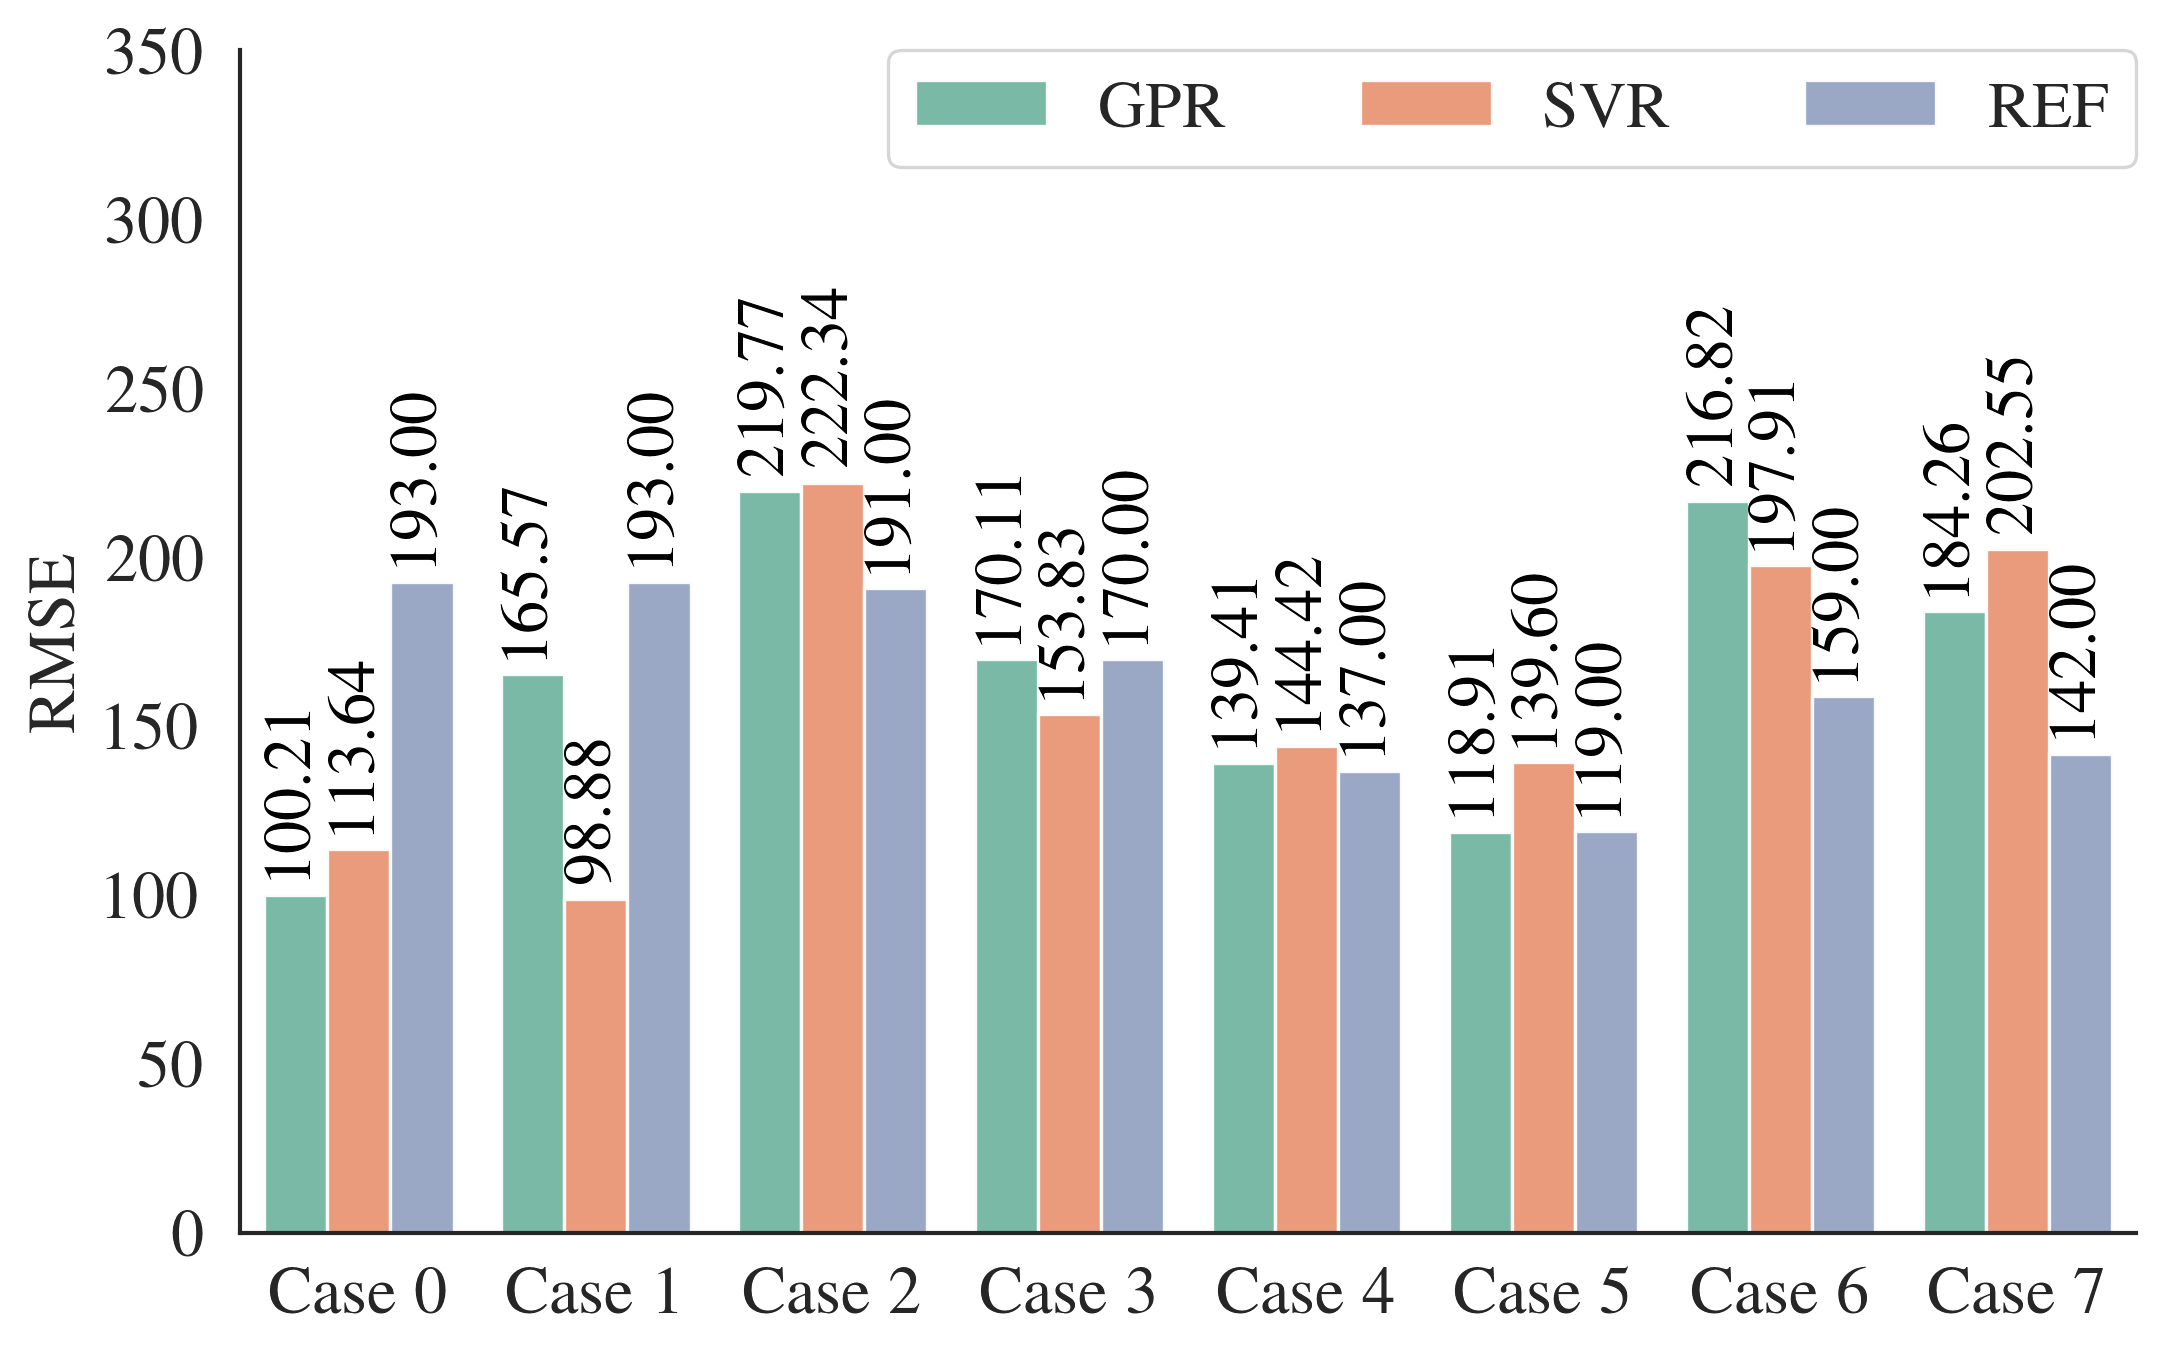
\includegraphics[width=0.495\linewidth]{./results/eml____300dpi_comparison_datasets_metric_rmse_bar}
 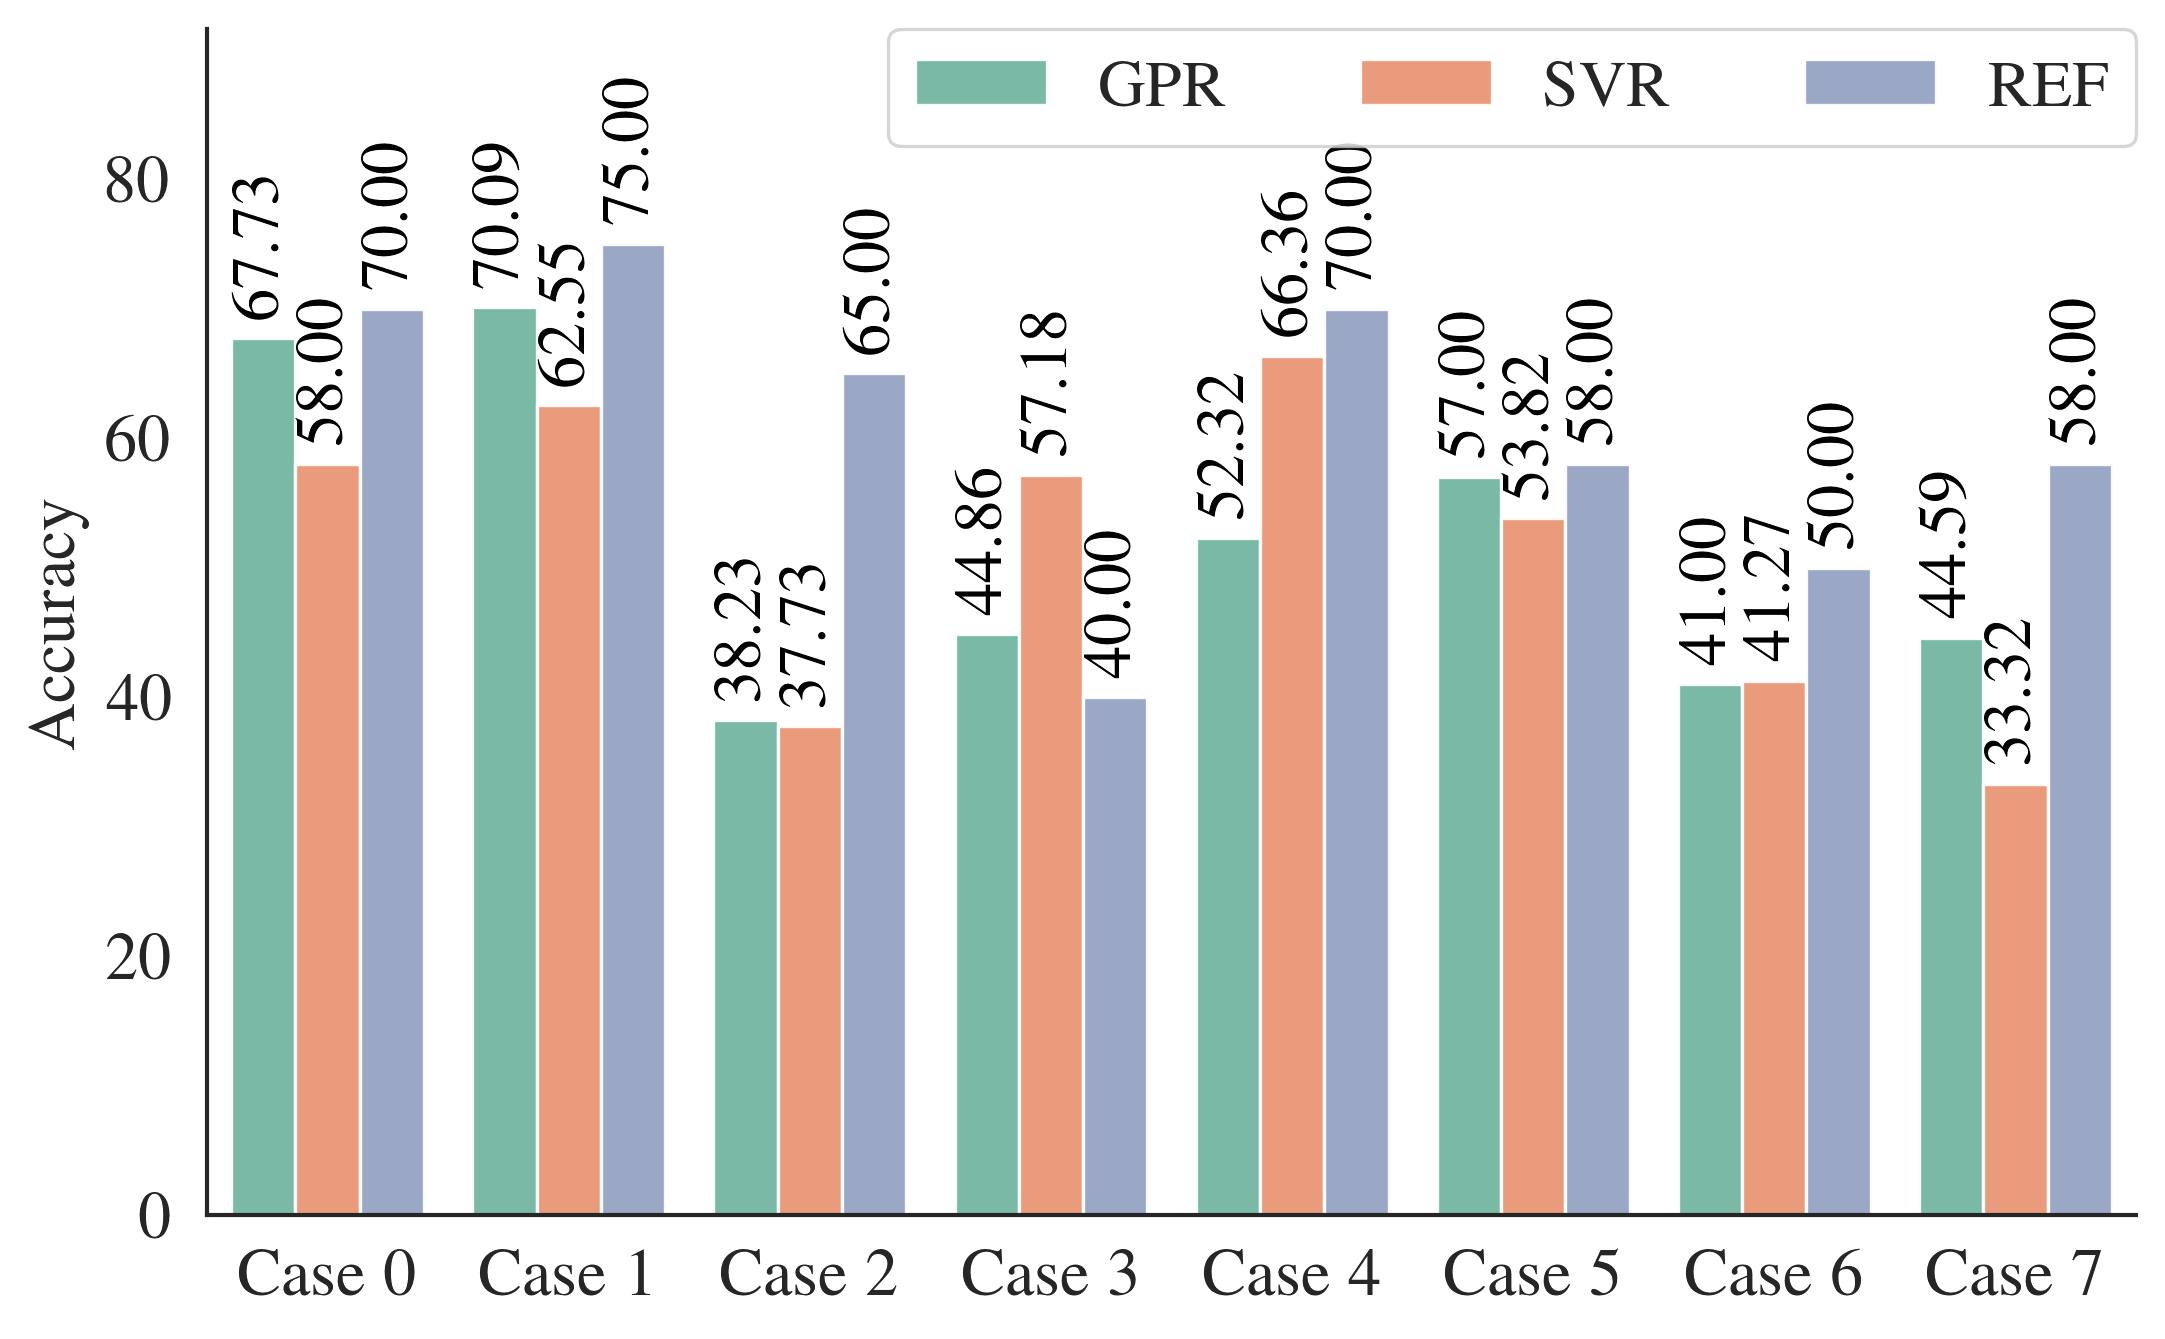
\includegraphics[width=0.495\linewidth]{./results/eml____300dpi_comparison_datasets_metric_accuracy_bar}
 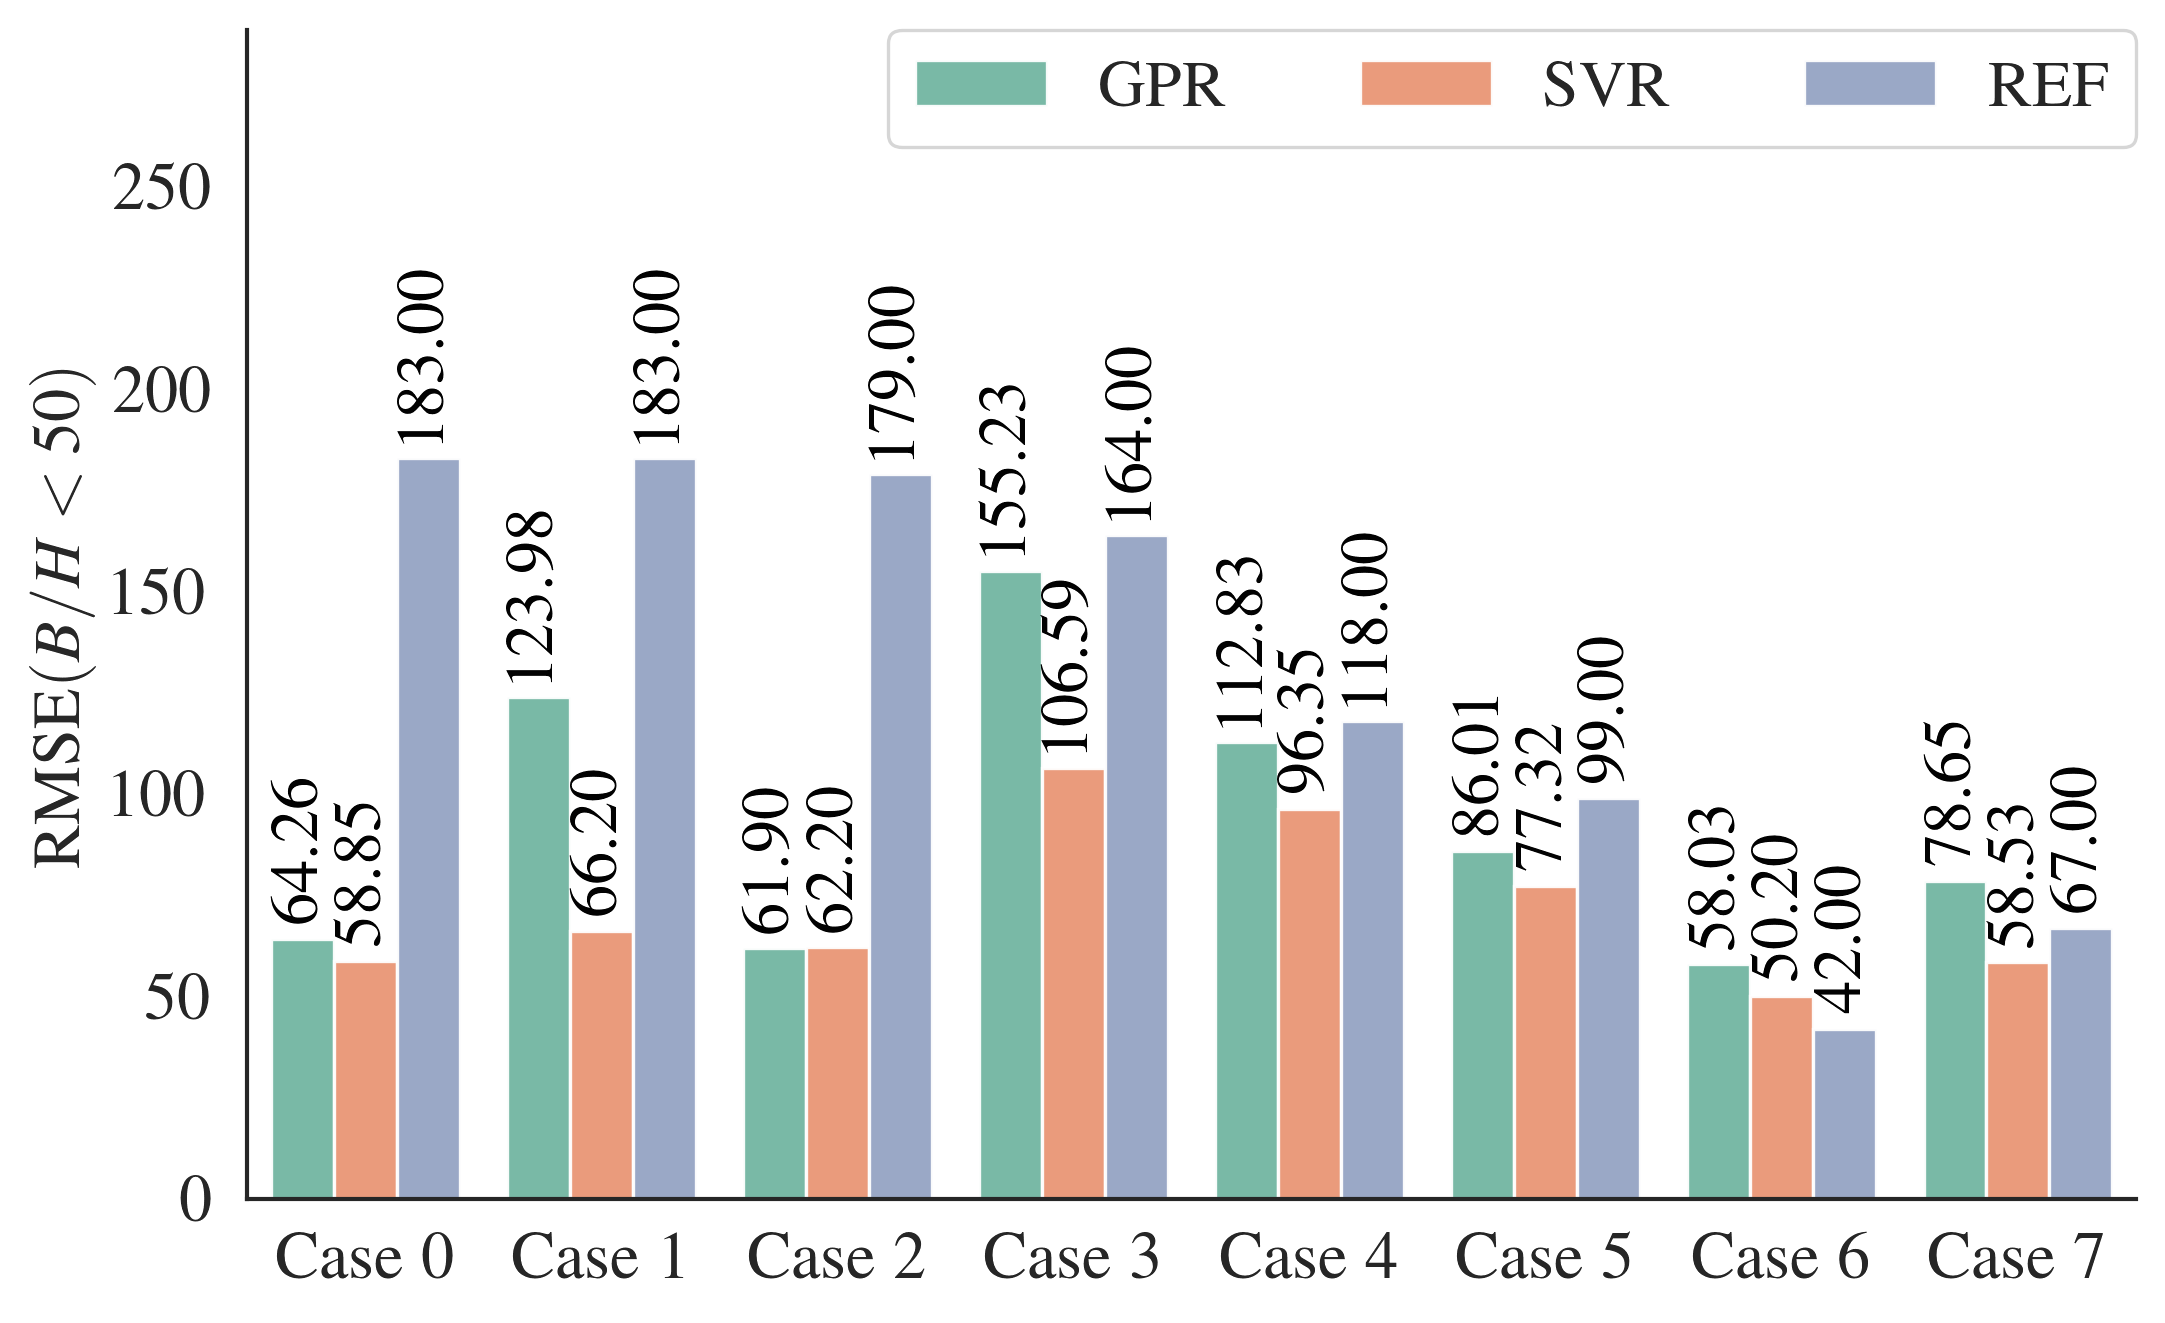
\includegraphics[width=0.495\linewidth]{./results/eml____300dpi_comparison_datasets_metric_rmsebh_50_bar}
 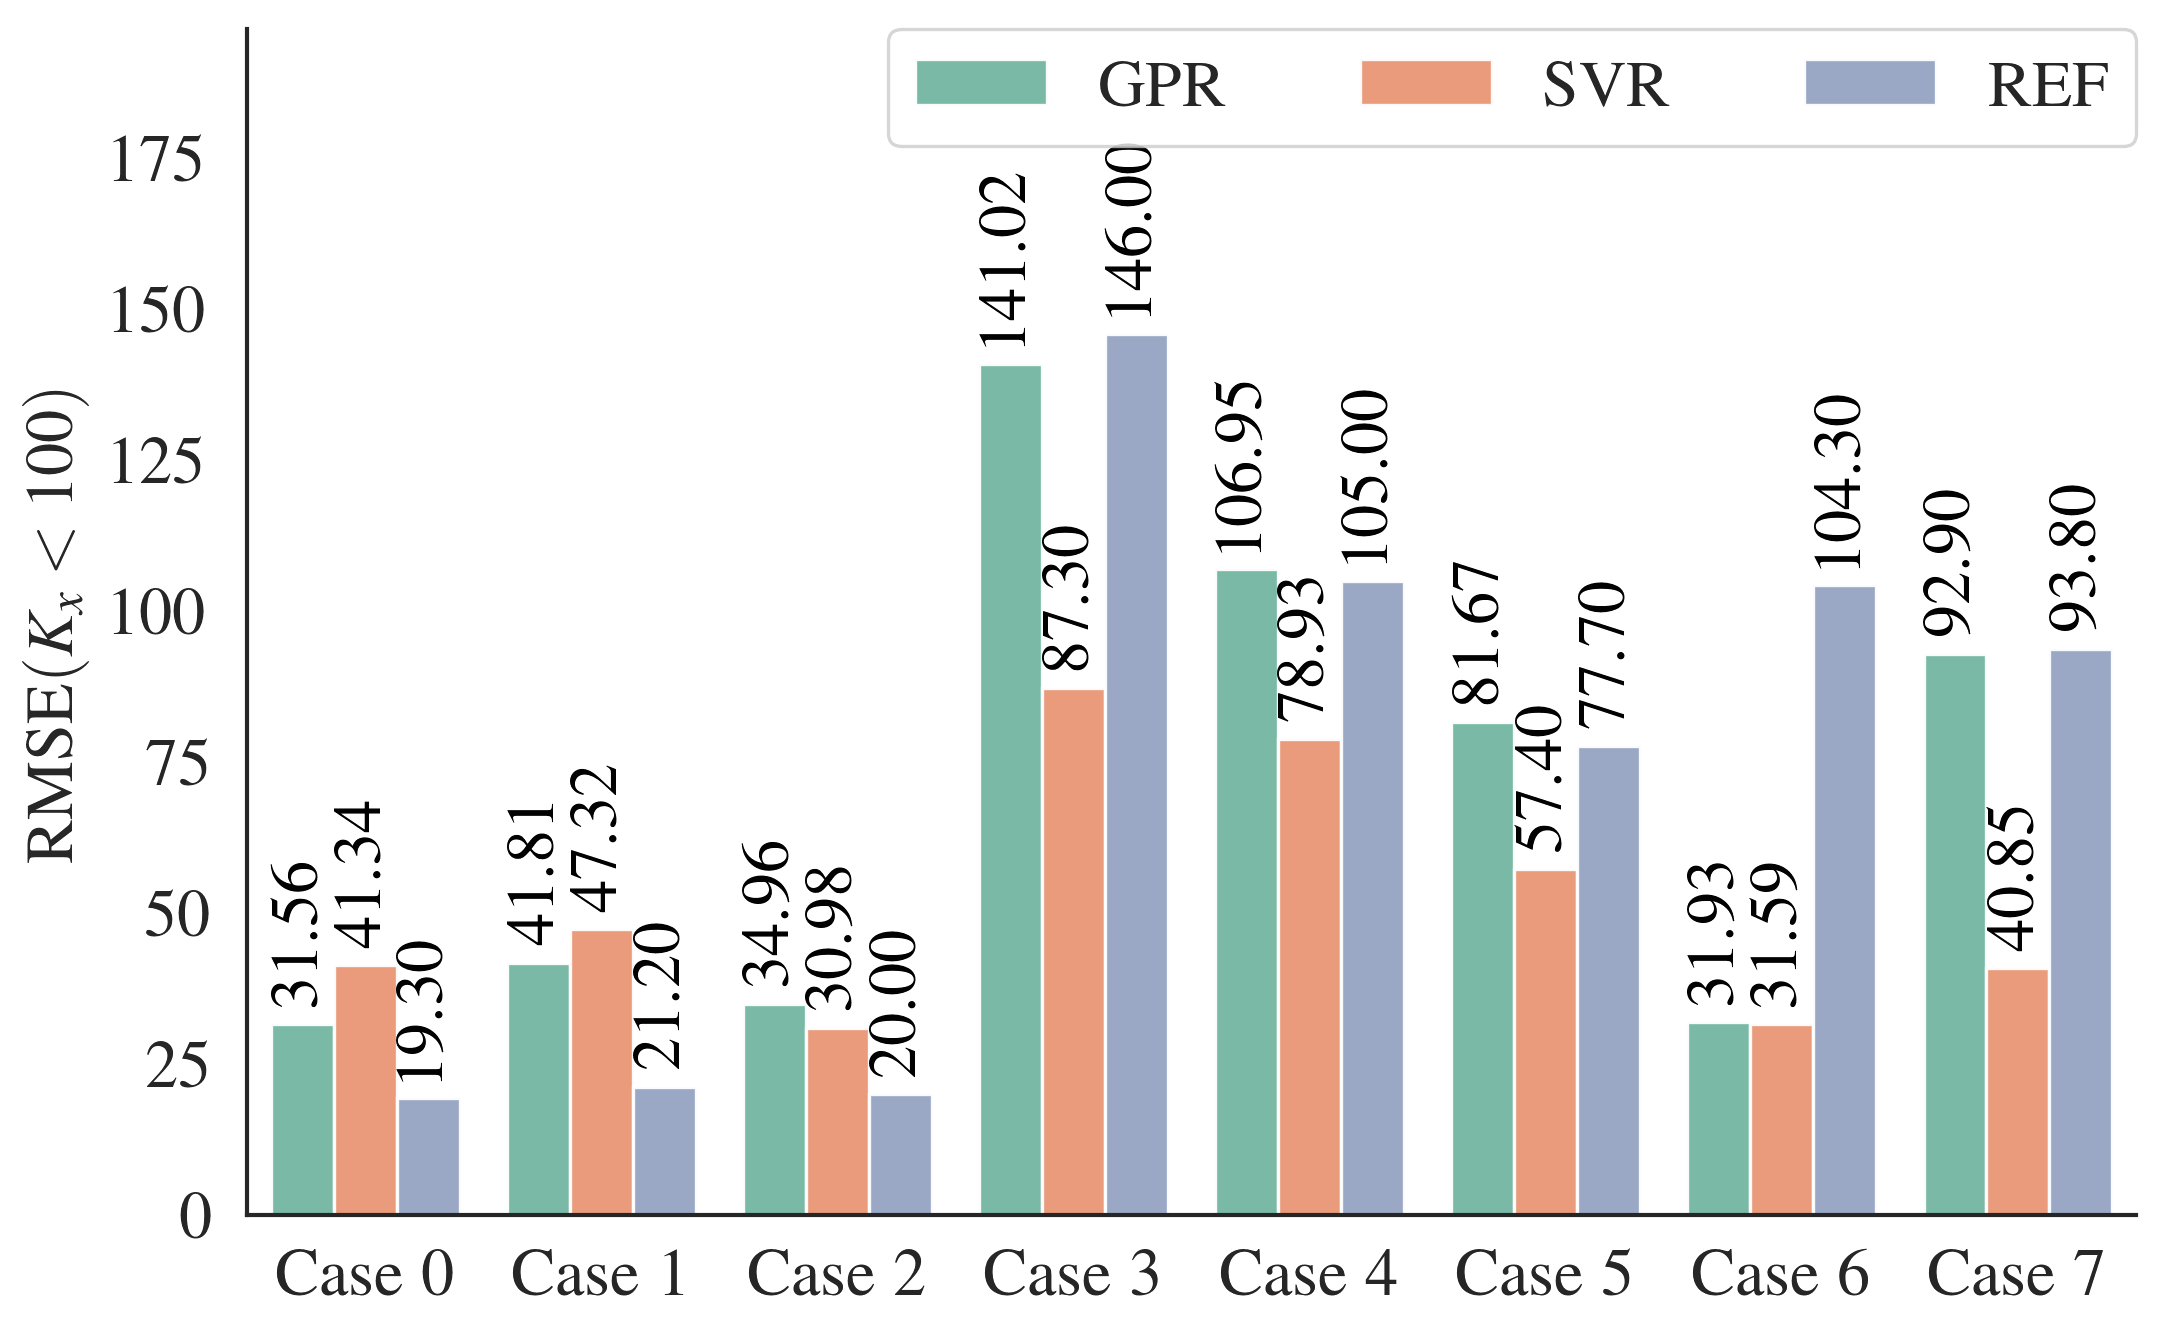
\includegraphics[width=0.495\linewidth]{./results/eml____300dpi_comparison_datasets_metric_rmsek_x_100_bar}
 \caption{
 \label{fig:eml____300dpi_comparison_datasets_metric}
 Longitudinal Dispersion Coefficient modeling using GPR and SVM.
%  The variable setups  for Cases 1-7 were proposed in \cite{tayfur2005predicting}.
 The results indicated with label REF were collected from \cite{tayfur2005predicting}. 
%  The results for GPR and SVR were averaged over 100 independent runs.
 }
\end{figure}


Figure \ref{fig:eml____300dpi_comparison_datasets_metric}
compares the results for $K_x$ modeling without feature selection.
% The variable setups are shown in Table \ref{tab:cases-features}.
In this figure, the results for GPR and SVR were averaged over 100 independent runs.
%  
According to Figure \ref{fig:eml____300dpi_comparison_datasets_metric}, we can observe for Case 0, the average value of RMSE is considerably lower than those produced by the reference model for both GPR and SVR models. The averaged accuracy obtained with GPR model was competitive with those produced by the reference model, but there was a decrease in performance for the accuracy of the SVR model. Notably, for the case where the width-to-depth ratios are small than 50, the RMSE $(B/H<50)$ values were remarkably better than the reference model, representing a decrease of 64.9\% for the GPR and 67.8\% for SVR. This finding shows that the hybrid method can provide accurate predictions for narrow channels. 
On the other hand, the hybrid model did not produce better results than the reference model when the extreme values were not considered, as can be observed for root mean squared errors less than 100 m$^2$/s, RMSE $ (K_x <100)$. 

The results for Case 1 are interesting since the features used as input variables in this model are a subset of the collected ones.  The features use in this model, $U$, $H$ and $B$, are those exhibit  higher correlations with the dispersion coefficient as can be seen in Figure \ref{fig:eml____300dpi_correlation_target___k_x}. Figure \ref{fig:eml____300dpi_scatter_target} show the strength of the linear relationships for $U$, $H$ and $B$.
It is important to notice that, although informative, the linear correlation may not be able to represent the complex and nonlinear nature of $K_x$ \cite{noori2016reliable}. 

Considering the results in Figure \ref{fig:eml____300dpi_comparison_datasets_metric}, although GPR performed better in accuracy, SVR produced smaller RMSE when compared to GPR and the reference model.
In addition, GPR predicts poorly the dispersion coefficient for narrow channels, as can be observed in the higher values for RMSE if $(B/H<50)$ compared to SVR.
However, considerint the RMSE $(B/H<50)$, both models produced better predictions then the reference model. 
% 
\begin{figure}[h] 
 \centering
 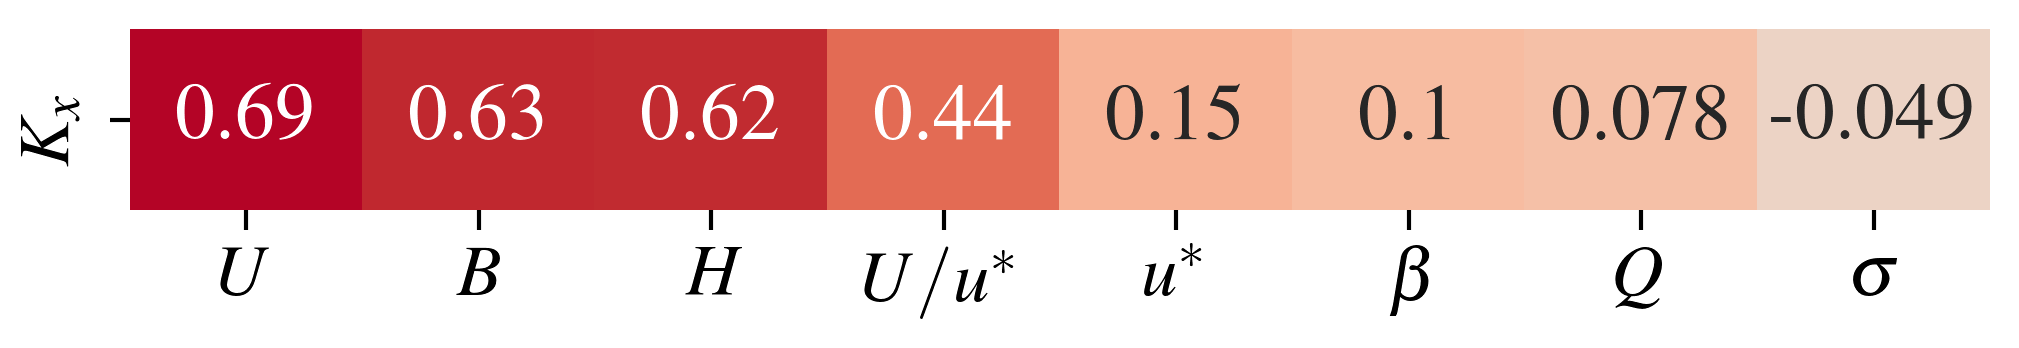
\includegraphics[width=0.6\linewidth]{./results/eml____300dpi_correlation_target___k_x}
 \caption{
 \label{fig:eml____300dpi_correlation_target___k_x}
 Correlation coefficients  using Spearman rank correlations between the eight input variables and the longitudinal dispersion coefficient.
 } 
\end{figure}
% 
\begin{figure}[h]
 \centering
 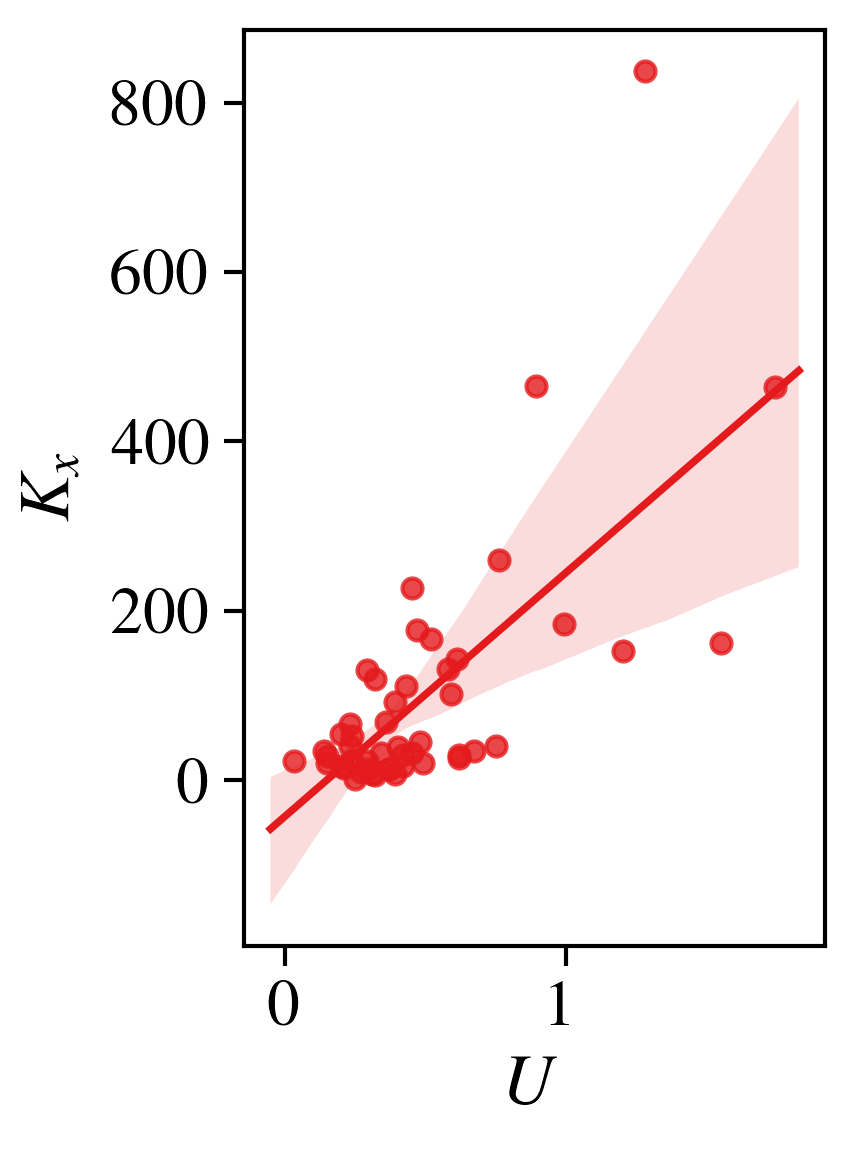
\includegraphics[width=0.24\linewidth]{./results/eml____300dpi_scatter_target_u_k_x}
 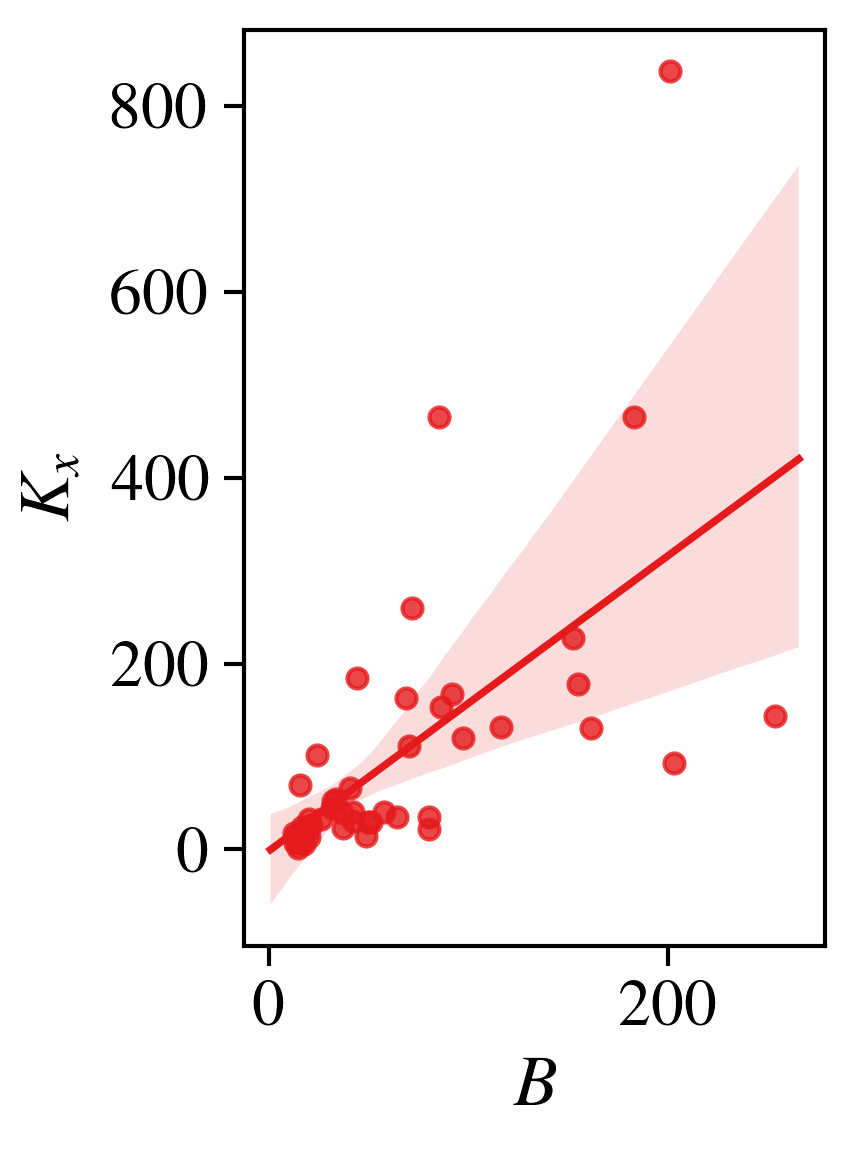
\includegraphics[width=0.24\linewidth]{./results/eml____300dpi_scatter_target_b_k_x}
 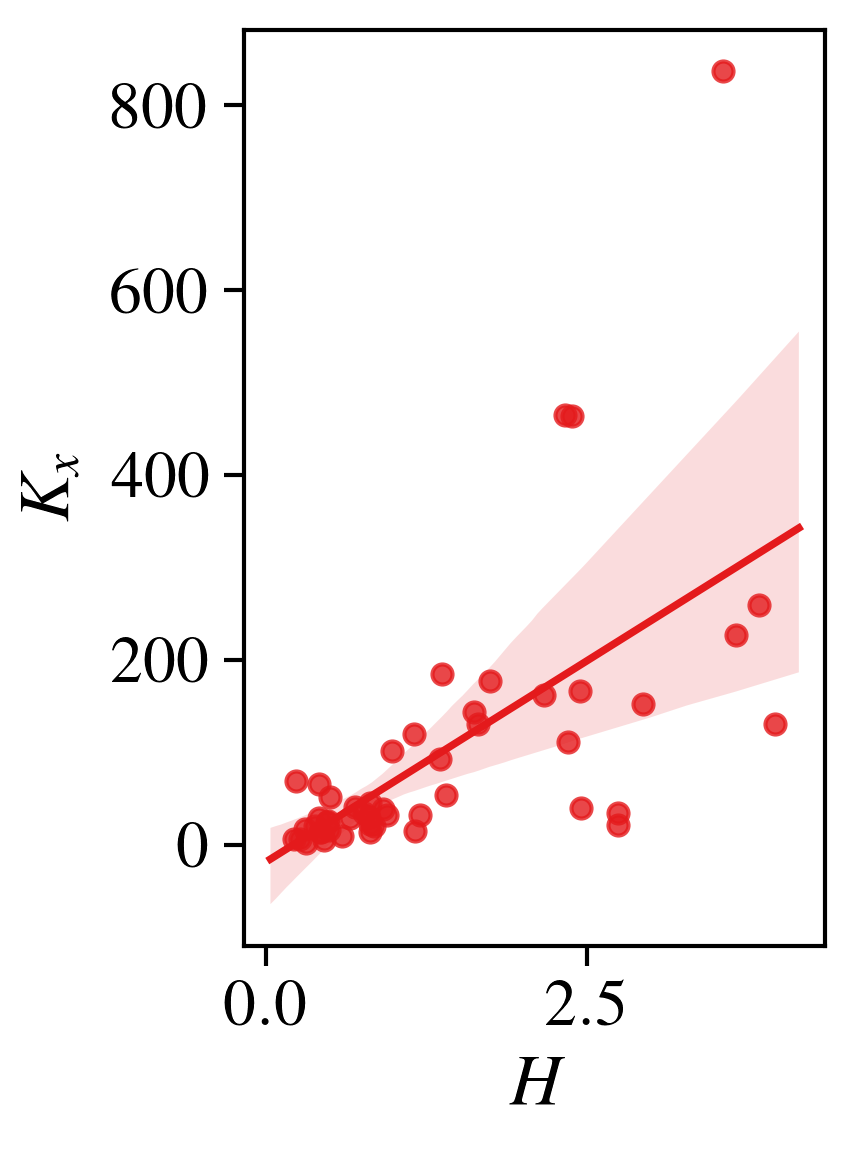
\includegraphics[width=0.24\linewidth]{./results/eml____300dpi_scatter_target_h_k_x}
 \caption{
 \label{fig:eml____300dpi_scatter_target}
 Scatter plots demonstrating visually the relationship among $U$, $B$, and $H$ features and the dispersion coefficient.
 }
\end{figure}


For Cases 2, 3, and 6, the hybrid approach performed poorly. 
It is interesting to notice that Case 2 involves the features implicitly in Case 1 since the flow discharge is the product of flow
depth, velocity, and channel width, $Q = HUB$.  
In addition, the linear correlation between the flow discharge and the dispersion can be discarded due to the small correlation as shown in Figure  \ref{fig:eml____300dpi_correlation_target___k_x}. 
The models for Cases 2, 3, and 6 are built upon one variable, which is not enough to represent the nonlinear relationship between the single feature and the dispersion coefficient. The finding corroborates the results described in \cite{tayfur2005predicting}, that solely the flow discharge ($Q$), flow velocity ($U$), and the relative shear velocity ($u^*$) are not sufficient to predict the nonlinear behavior of the dispersion coefficient.

Cases 4 is built upon Case 3, with the inclusion of the channel shape parameter ($\beta$) for Case 4, while in Case 5, the channel sinuosity is added to Case 4.
The hybrid model performed similarly to the artificial neural network developed in the reference paper. However, it was not able to improve the results when compared to the previous cases.  

Case 7 considered the relative shear velocity ($U/u^*$) as in Case 6,  and channel shape parameter ($\beta$)  along with the channel sinuosity ($\sigma$) to predict the dispersion coefficient. The metrics shown in Figure \ref{fig:eml____300dpi_comparison_datasets_metric} show the inclusion of the channel shape parameter and the channel sinuosity did not improve the $K_x$ estimations.


The results depicted in Figure \ref{fig:eml____300dpi_comparison_datasets_metric} obtained after several independent runs allows for draw the following conclusions on the test Cases presented in Table \ref{tab:cases-features}. 
% 
From Cases 0-7, GPR and SVR  have produced the overall best results for Case 0 and Case 1, as can be seen in Figure \ref{fig:eml____300dpi_comparison_datasets_metric}. 
Given the performance of the GPR and SVR models in Cases 0 and 1, the comparative analysis will be focused on these two cases.
The Root Mean Squared Error of both models was inferior to the artificial neural network developed in \cite{tayfur2005predicting}. 
In Case 0,  where the eight variables are taken into account, the GPR and SVR models showed an average reduction of 58.9\% and 58.8\% for the RMSE, respectively. Similar behavior was observed for narrow channels where $ B / H <50 $: the reduction was 35.1\% and 32.2\% for GPR and SVR, respectively. Also,  the averaged Accuracy for GPR  is only 3.24\% small them the reference model. We emphasize that the results are the average of 100 independent runs.

In Case 1 the averaged RMSE  values obtained by GPR and SVR  were smaller than the RMSE attained by the reference model. However, the RMSE produced by GPR was higher than that provided by SVR. Similar behavior is observed for Root Mean Squared Error of narrow channels ($ B / H <50 $). For the same Case 1, GPR produced an averaged Accuracy of 70.09\% against 75\% for the reference model, resulting in a percentage difference of 6.55\% on average.  

For Cases 0 and 1,  Figure \ref{fig:eml____300dpi_scatter_best_model___ldc} depicts the scatterplots of the predicted and estimated dispersion coefficient for the best models  in the test set (according to RMSE).
Besides the RMSE, the accuracy and the coefficient of determination associated with each model are also shown. Although a few predicted $K_x$ present a visible error, the predictions for GPR and SVR models agree well with the observations. This can be verified by the R$^2$ values, above 0.90 for for GPR in Cases 0 and 1. For SVR, R$^2= 0.93$ for Case 0 and R$^2= 0.89$ for Case 1.
%
\begin{figure}[!htb] \centering 
 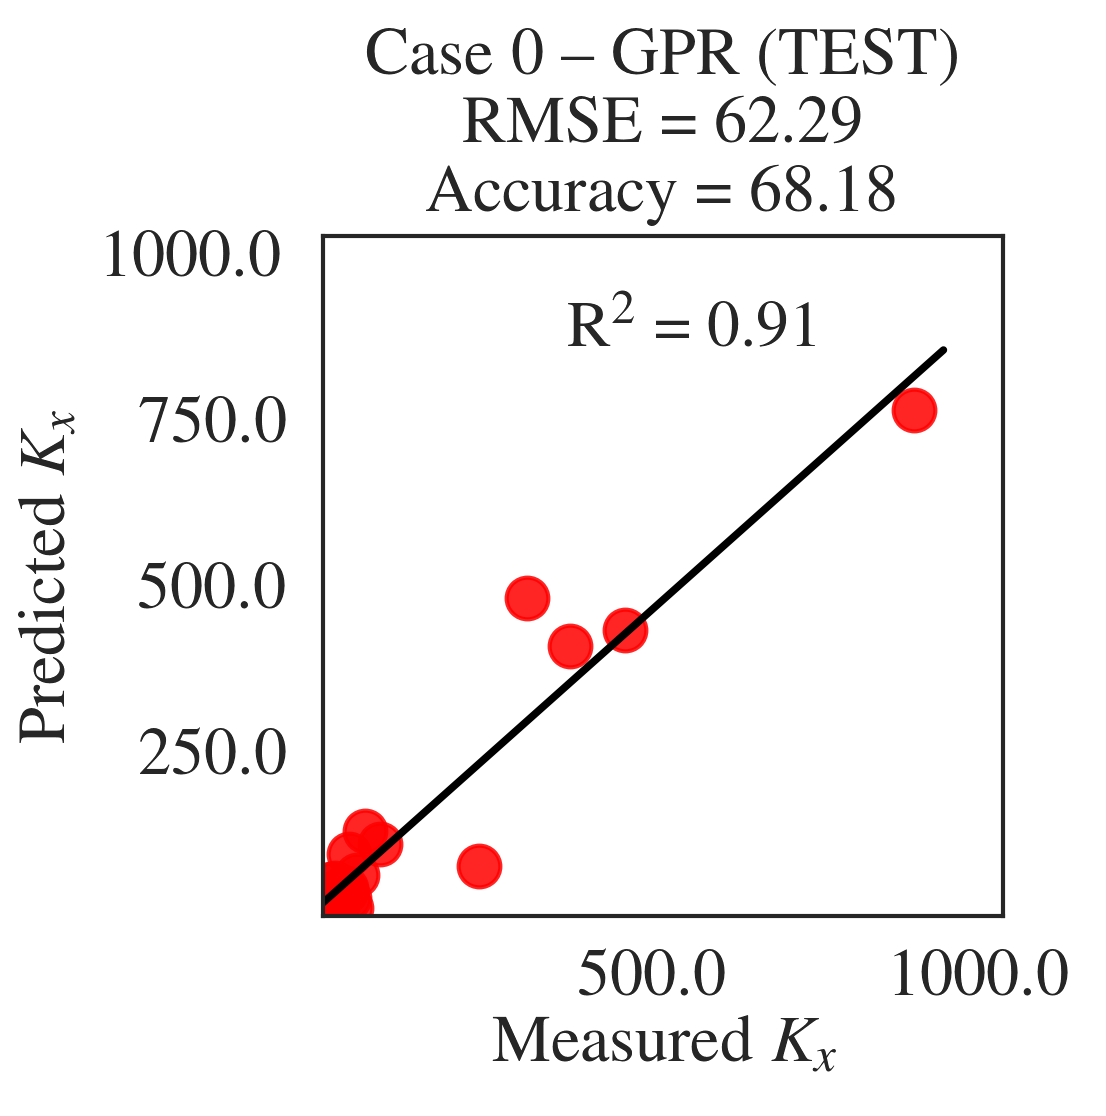
\includegraphics[width=0.33245\textwidth]{./scatter/eml____300dpi_scatter_best_model___gpr__case_0__test}
 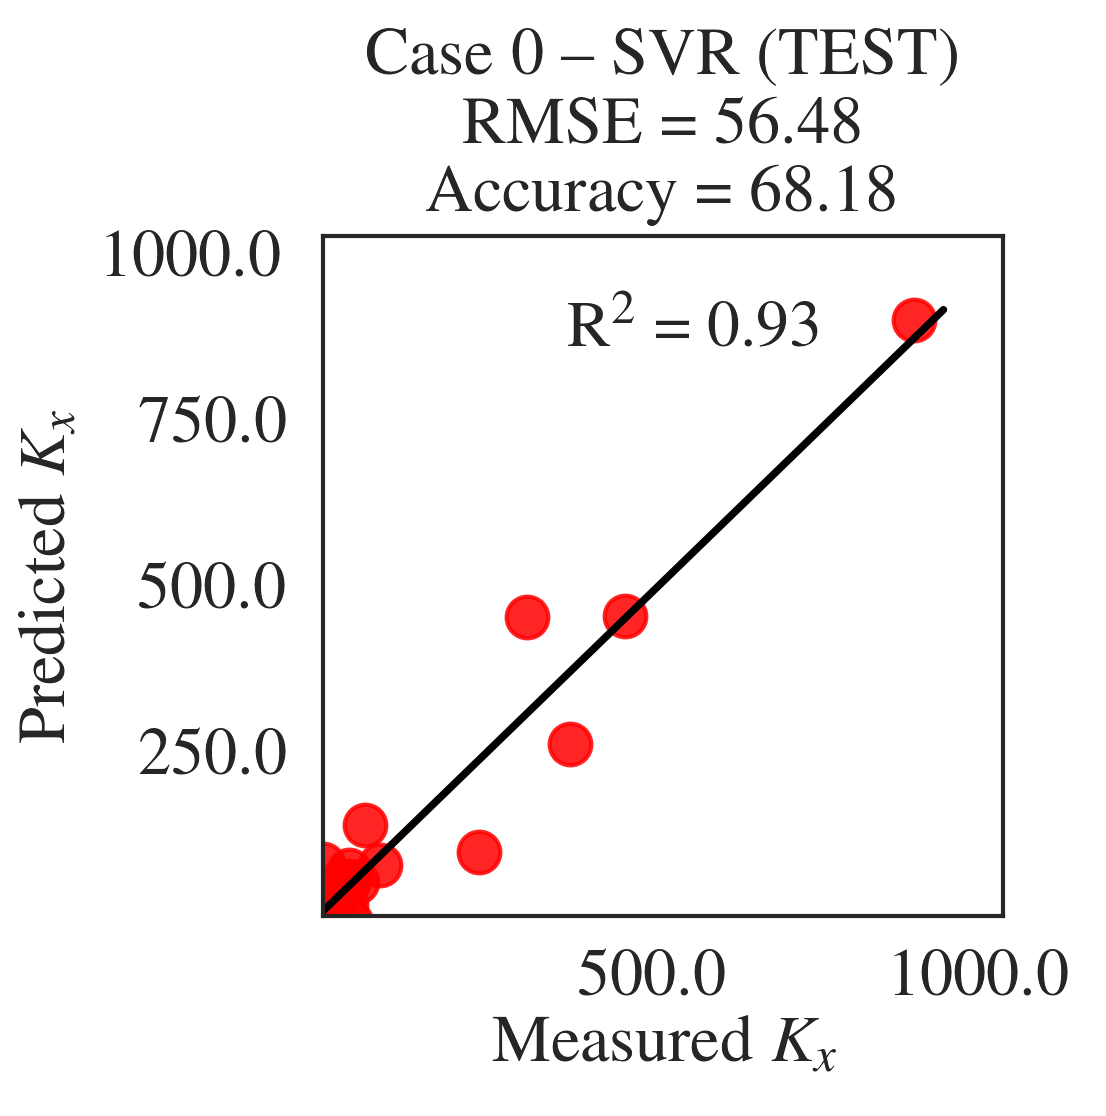
\includegraphics[width=0.33245\textwidth]{./scatter/eml____300dpi_scatter_best_model___svr__case_0__test}
 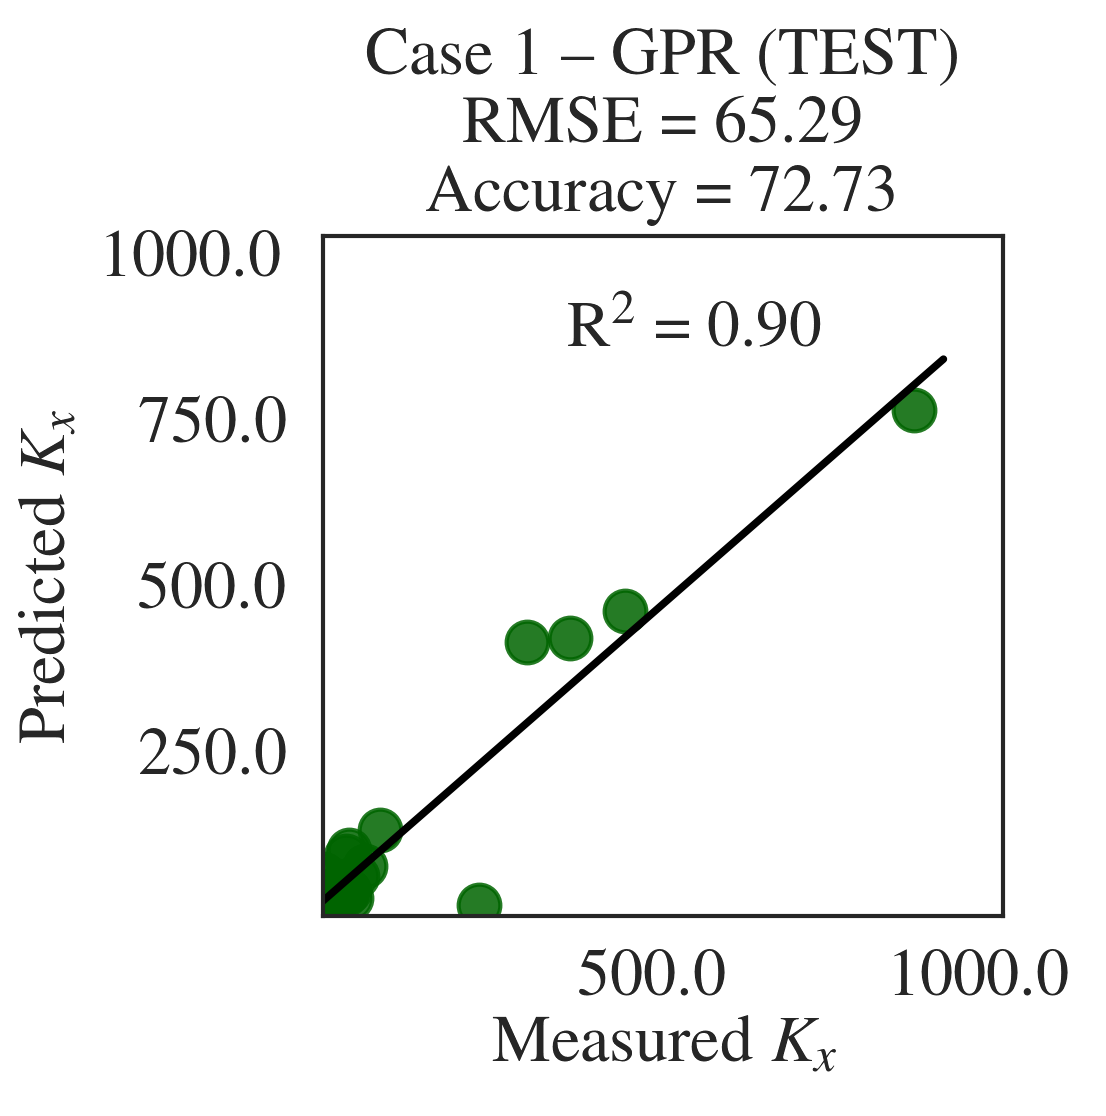
\includegraphics[width=0.33245\textwidth]{./scatter/eml____300dpi_scatter_best_model___gpr__case_1__test}
 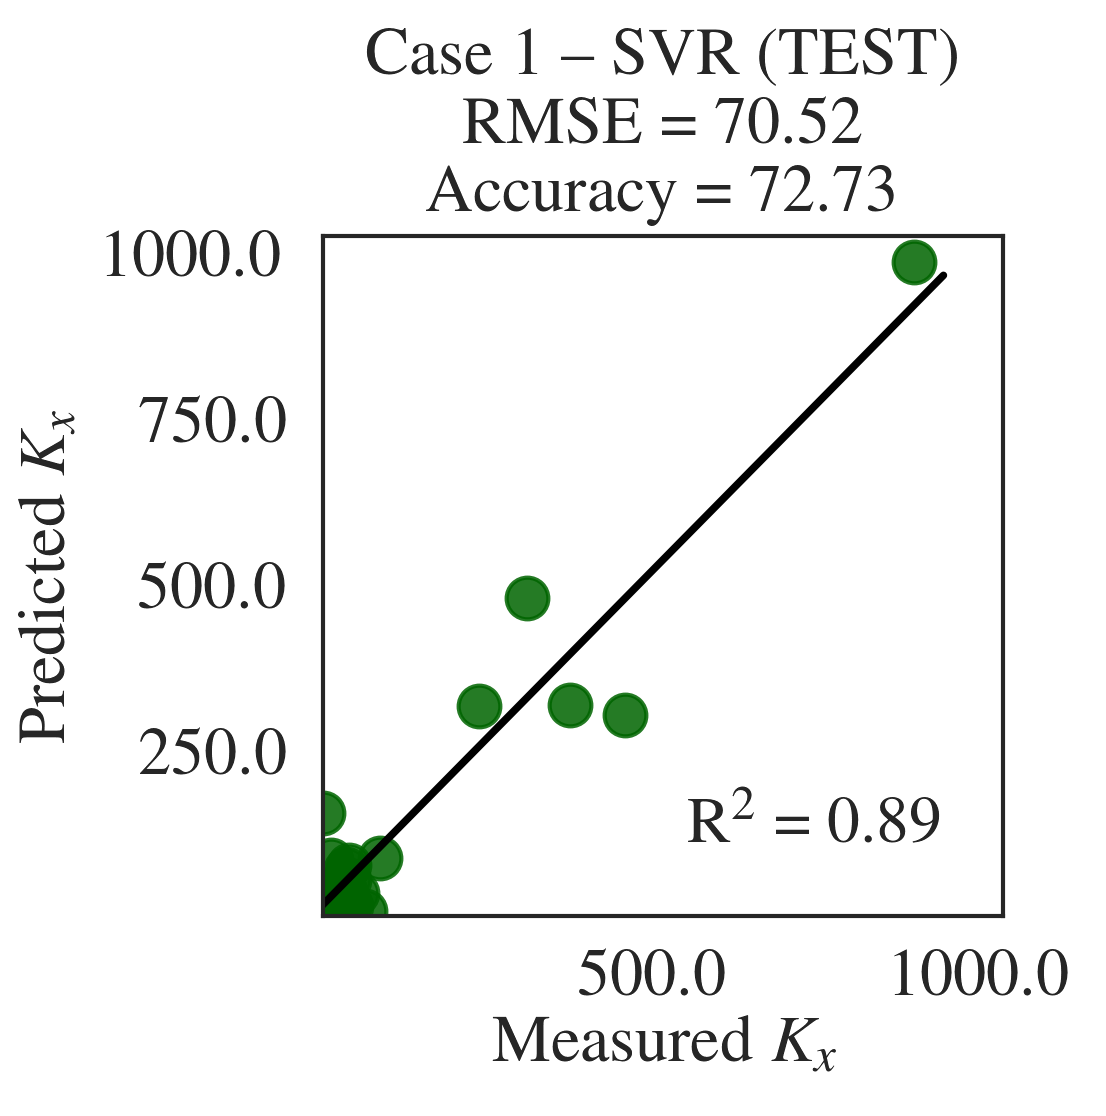
\includegraphics[width=0.33245\textwidth]{./scatter/eml____300dpi_scatter_best_model___svr__case_1__test}
 \caption{\label{fig:eml____300dpi_scatter_best_model___ldc}
 Scatter plots for the best models according to Root Mean Squared Error (RMSE).}
\end{figure}
 
In the computational experiments, a total of 100 independent runs were performed. As a consequence, it is interesting to analyze the distribution of the internal parameters in all executions.
As Cases 0 and 1 produced better results compared to the other ones, the discussion is focused on these cases.
% 
Figure \ref{fig:eml____300dpi_comparison_datasets_parameters___gpr__test} shows for Cases 0-7 the distribution of the GPR parameters, namely, $k_0$, $\nu$, $l$,  and $\alpha$. The first three parameters control the  shape of the kernel shown in Equation \ref{eq:gpr-kernel-matern}  used to compute the estimations, while $\alpha$, which is added to the diagonal of the kernel matrix during fitting,  rules the level of noise in the observations.
The parameter $ k_0 $ controls the magnitude of the GPR approximation and the final solutions showed similar distributions in cases 0 and 1.
Similar behavior was noticed for the parameter $ \alpha $ which is associated with noise in the observations. The dispersion is a measure associated with a natural process, so that noise becomes an important factor in the estimates.
The parameter $\nu$ is a critical paramater in the kernel function and controls the GPR smoothness \cite{stein-book:1999}: the smaller $\nu$ the less smooth the approximated solution is.
The distribution of $\nu$ in Figure \ref{fig:eml____300dpi_comparison_datasets_parameters___gpr__test} shows the GPR estimation functions produced for case for Case 1 are smoother than Case 0. 
In addition, the length scales $l$ for Case 1 are higher than Case 0 as well.
These combined circumstances potentially led to the highest RMSE values for case 1, as can be seen in Figure \ref{fig:eml____300dpi_comparison_datasets_metric}.
% 
\begin{figure}[!htb] \centering
  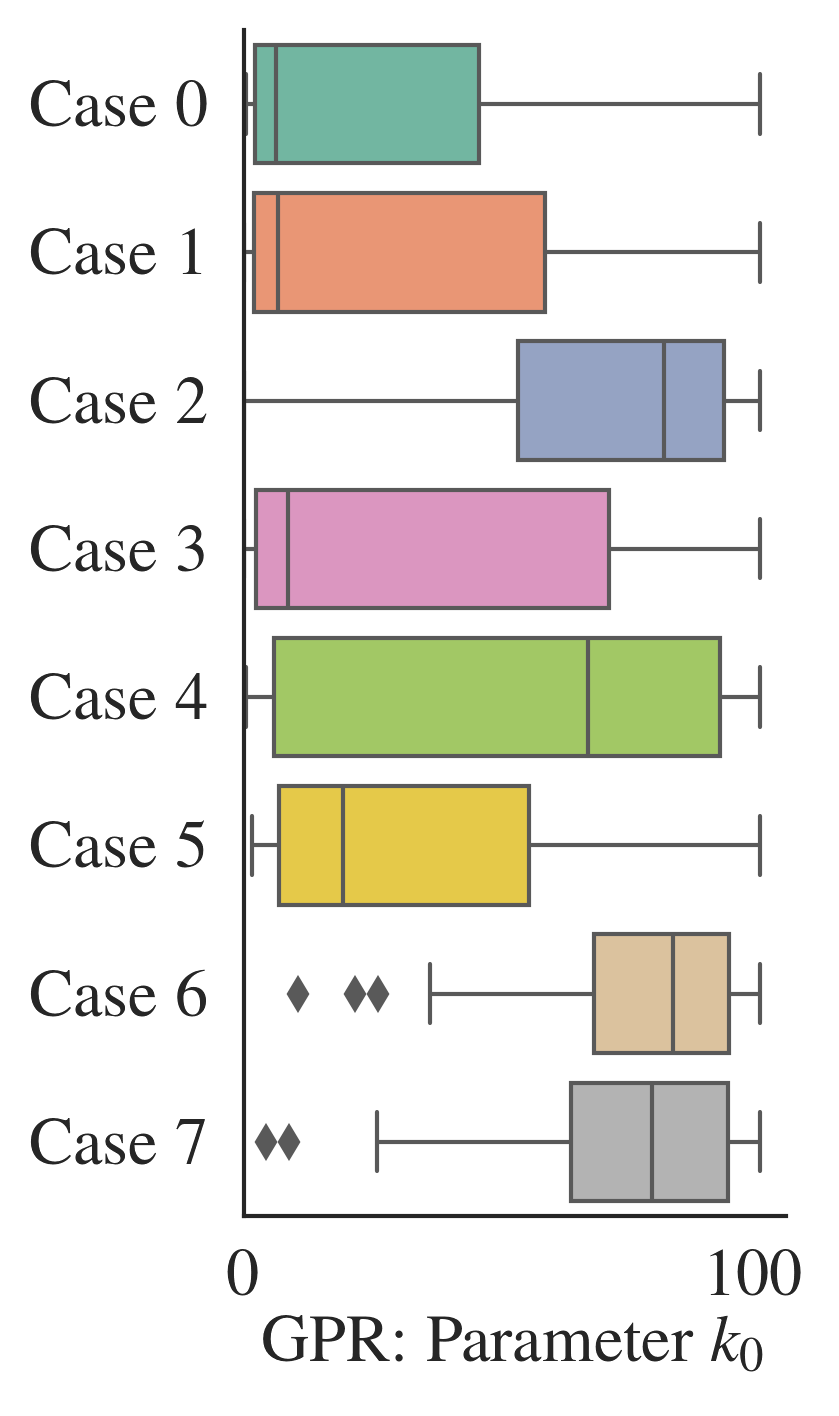
\includegraphics[width=0.2449\linewidth]{./results/eml____300dpi_comparison_datasets_parameters___gpr__k_0__test}
  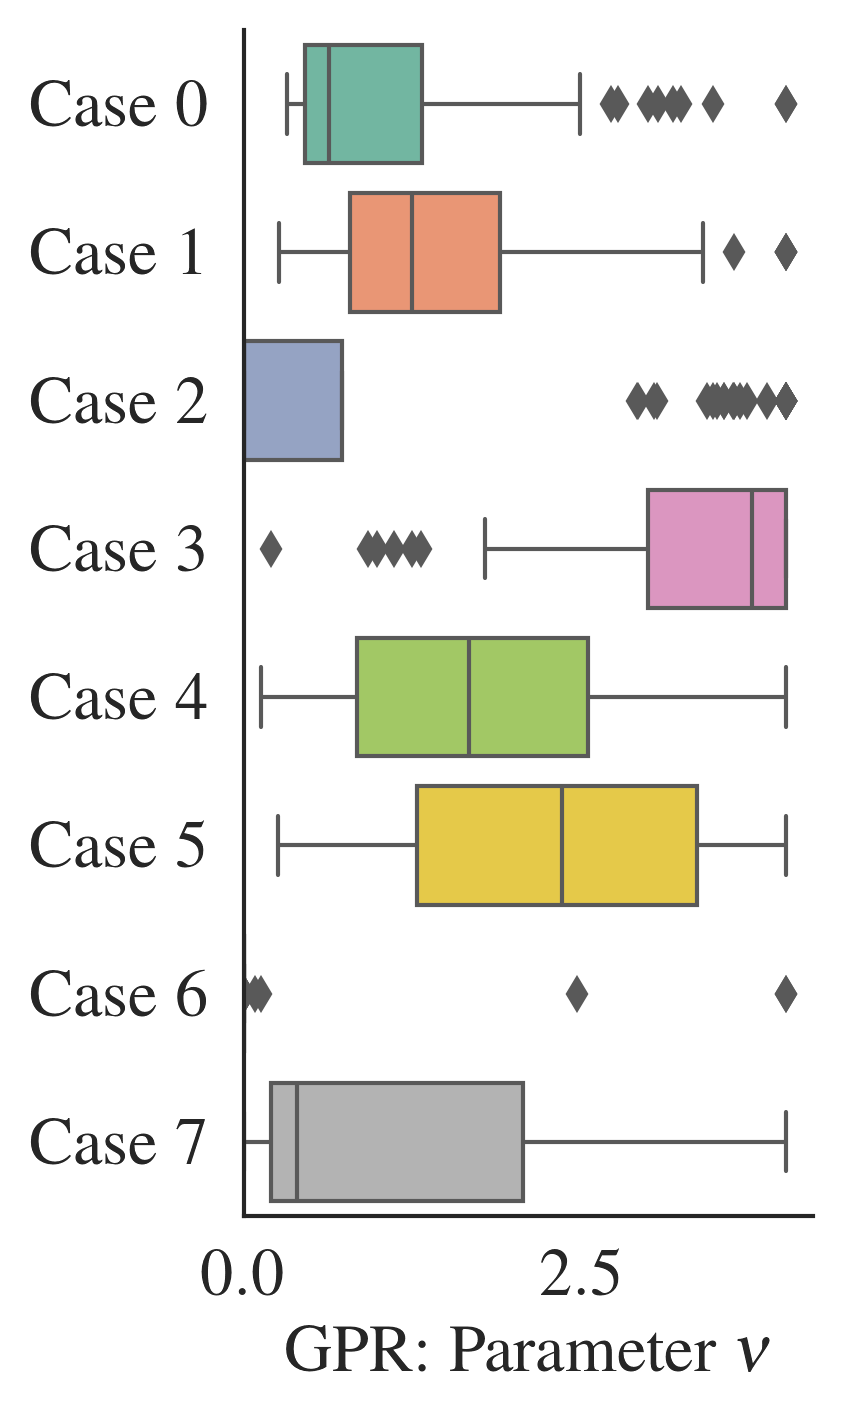
\includegraphics[width=0.2449\linewidth]{./results/eml____300dpi_comparison_datasets_parameters___gpr__nu__test}
  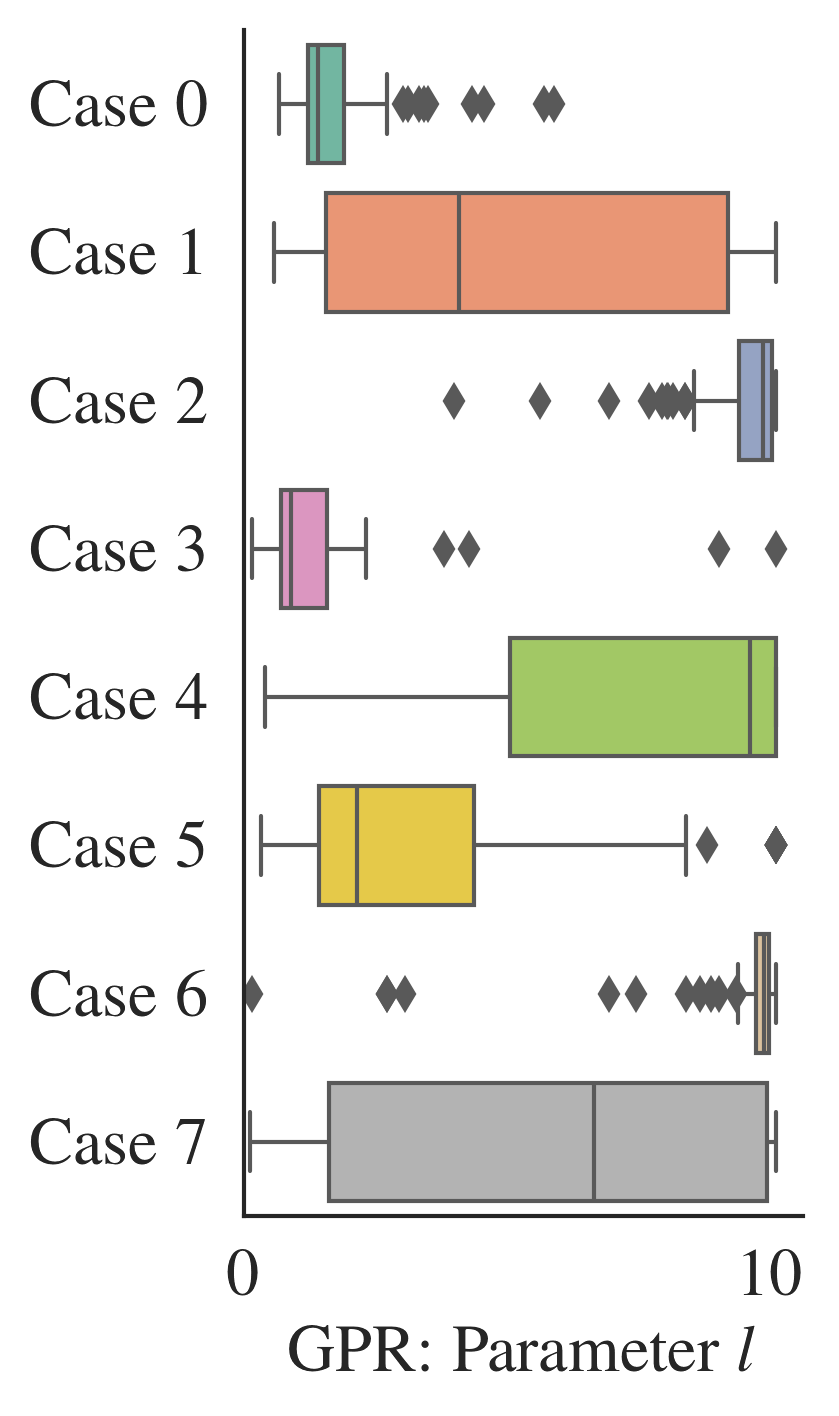
\includegraphics[width=0.2449\linewidth]{./results/eml____300dpi_comparison_datasets_parameters___gpr__l__test}
  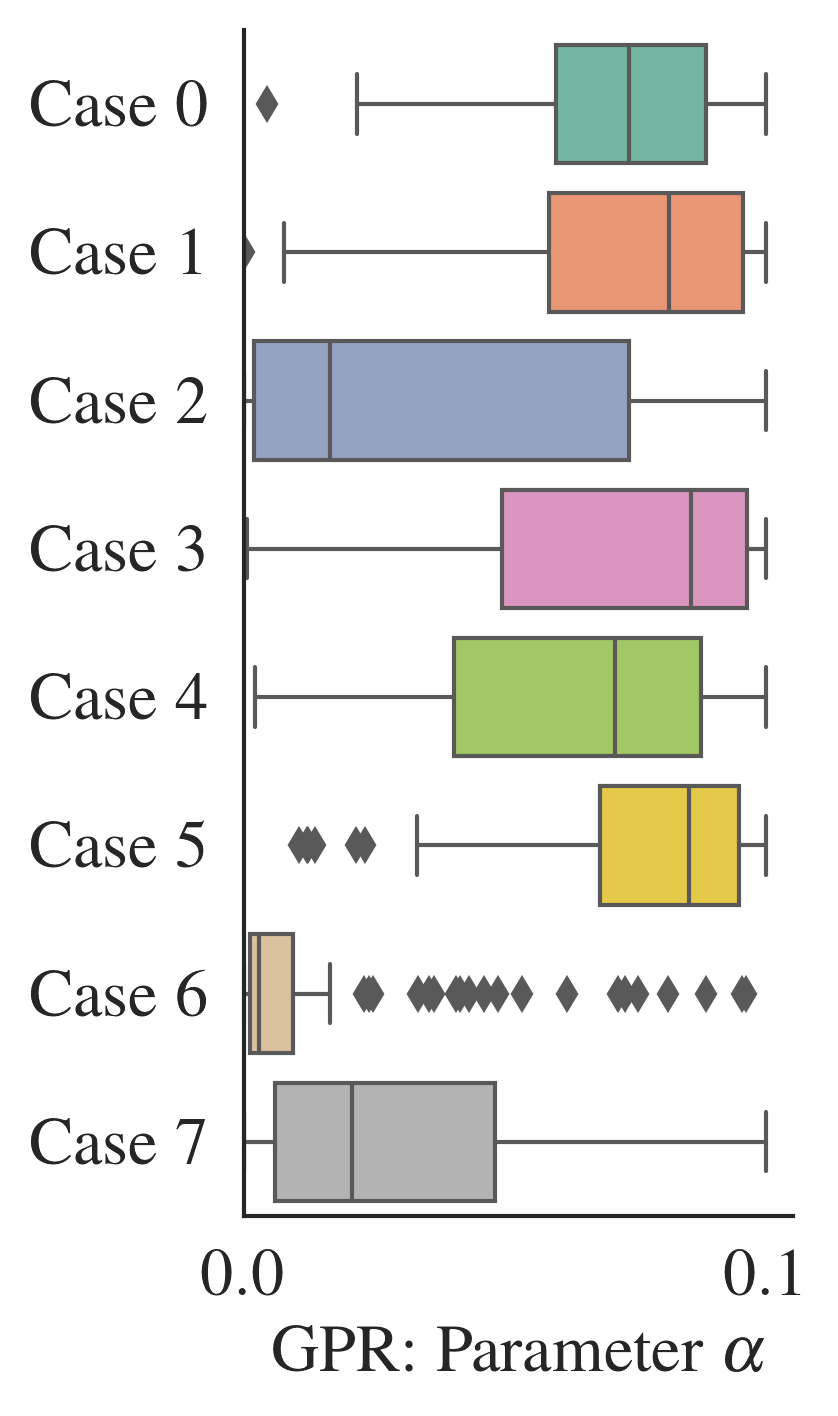
\includegraphics[width=0.2449\linewidth]{./results/eml____300dpi_comparison_datasets_parameters___gpr__alpha__test}
 \caption{\label{fig:eml____300dpi_comparison_datasets_parameters___gpr__test}
 Distribution of the internal parameters for the GPR models over 100 independent runs. 
 %The parameters and their respective ranges can be found in Table \ref{tab:cmaes__encoding}. 
 }
\end{figure}


Figure \ref{fig:eml____300dpi_comparison_datasets_parameters___svr__test} displays the distribution of the SVR internal parameters $C$, $\gamma$ and $\varepsilon$.
$C$ is the penalization parameter, $\varepsilon$ is the  specifies the penalization  associated in the training loss function,  and $\gamma$ is kernel coefficient in Equation (\ref{eq:svr-kernel}).
Analyzing the boxplots, one can observe the distribution of the parameters $\gamma$ and $\varepsilon$ showed similar distributions in both cases.
On the other hand, the values of parameter $C$  for Case 1 are higher than those found for Case 0.
In support vector machines, $C$  plays an important role as a regularization parameter. The regularization strength is inversely proportional to $C$. As a result, the SVR estimations for Case 0 are smoother than those produced for Case 1. The smaller RMSE values for Case 1  shown in the barplots in Figure  \ref{fig:eml____300dpi_comparison_datasets_parameters___svr__test} (averaged in 100 runs) supports this interpretation. 
% 
\begin{figure}[!htb] \centering
 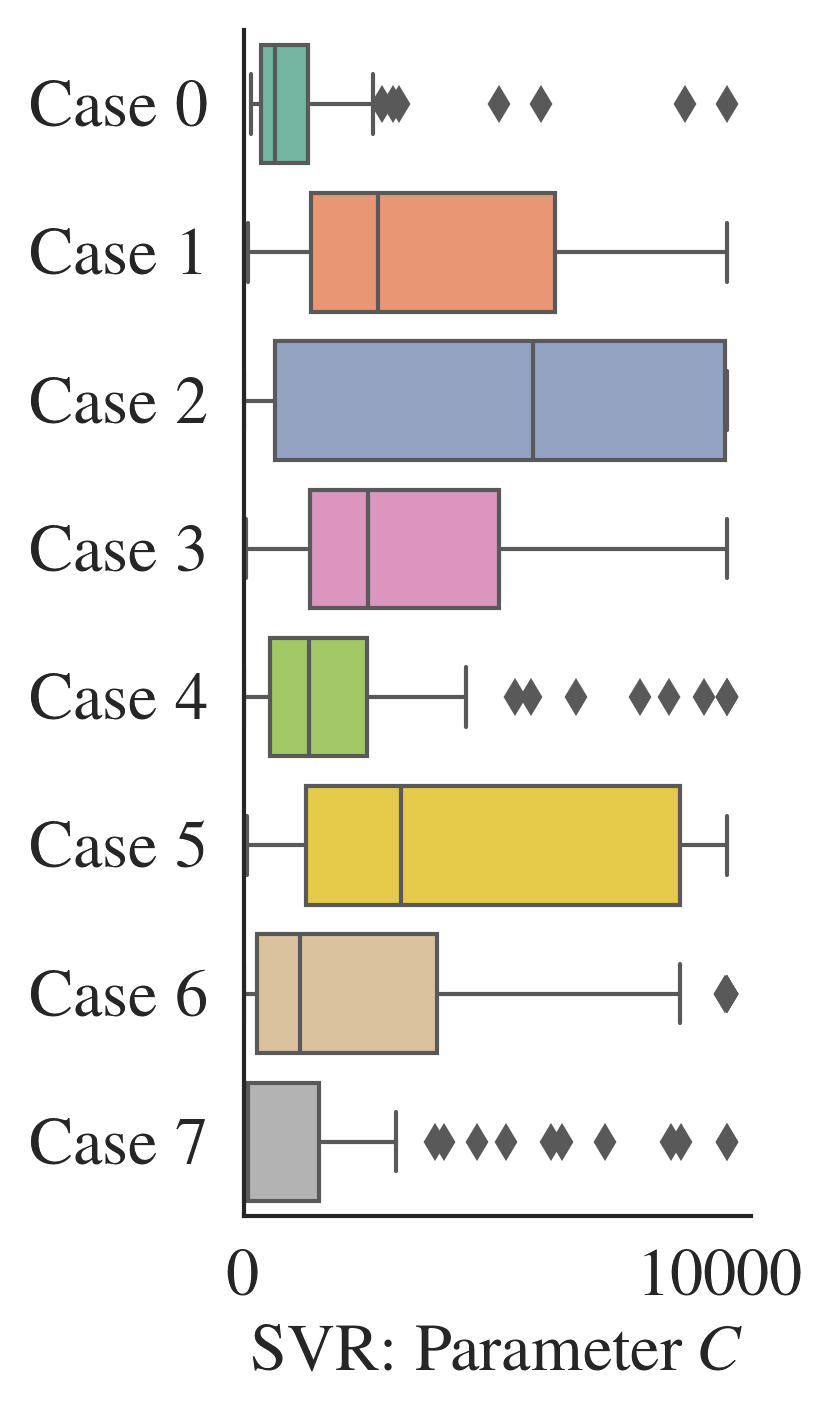
\includegraphics[width=0.2449\linewidth]{./results/eml____300dpi_comparison_datasets_parameters___svr__c__test}
 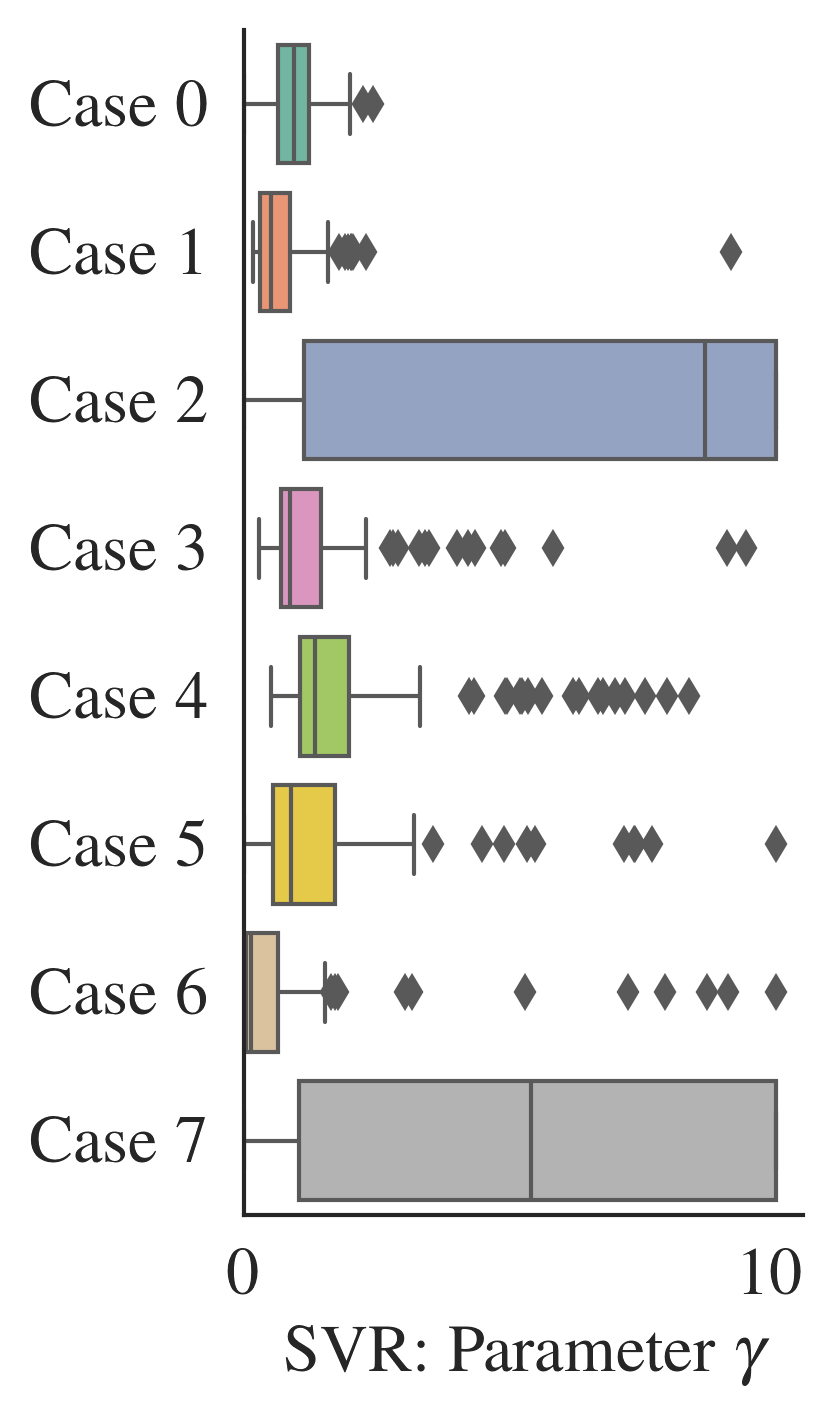
\includegraphics[width=0.2449\linewidth]{./results/eml____300dpi_comparison_datasets_parameters___svr__gamma__test}
 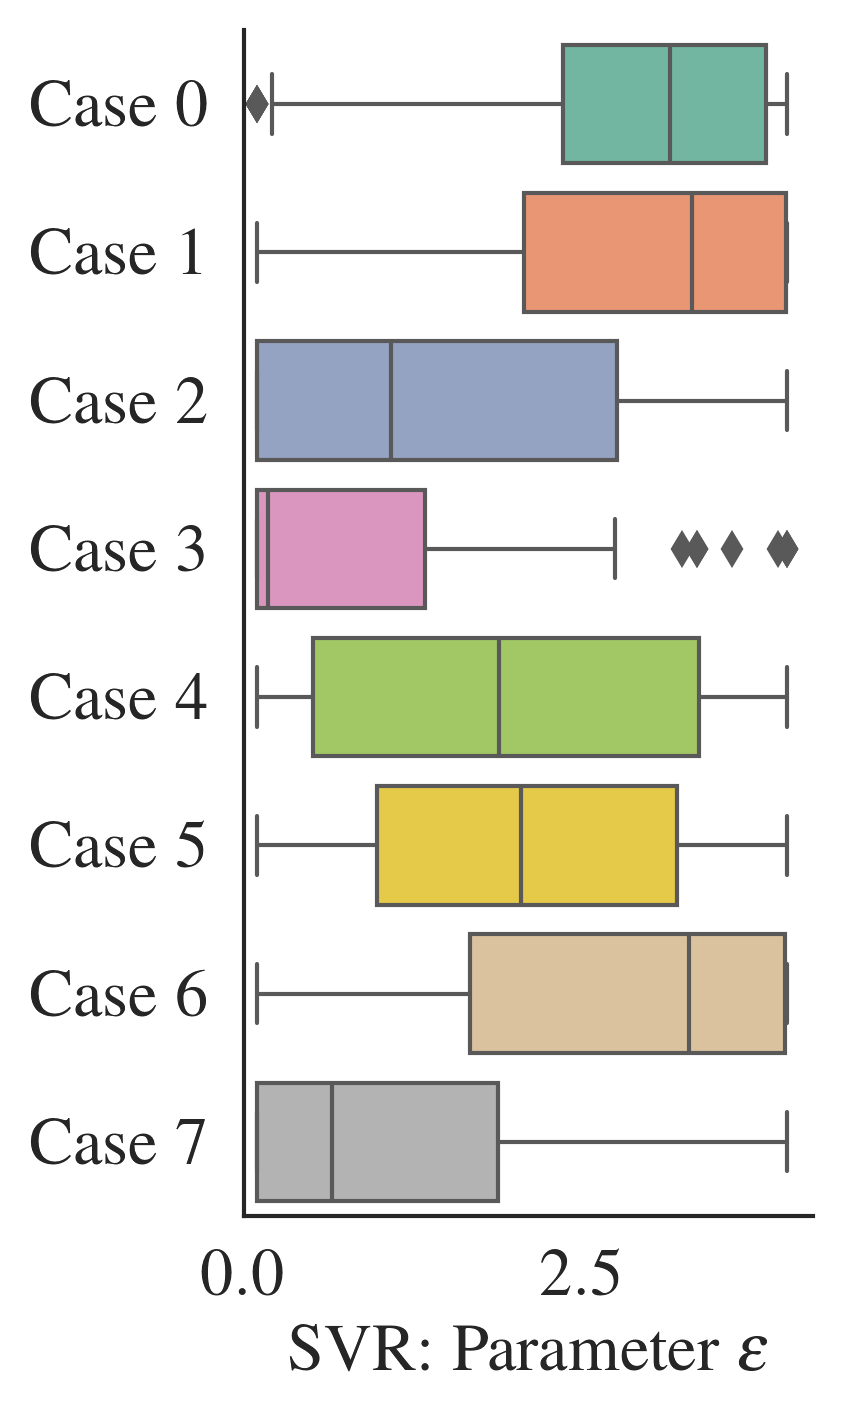
\includegraphics[width=0.2449\linewidth]{./results/eml____300dpi_comparison_datasets_parameters___svr__varepsilon__test}
 \caption{\label{fig:eml____300dpi_comparison_datasets_parameters___svr__test}
 Distribution of the internal parameters for the SVR models over 100 independent runs. 
 %The parameters and their respective ranges can be found in Table \ref{tab:cmaes__encoding}. 
 }
\end{figure}

When compared to the reference model, it can be observed that  GPR and SVM  presented a lower performance in predicting the dispersion coefficient when the extreme values ( $K_x > 100$) are discarded for Cases 0 and 1.  One possible explanation to the deprecated performance of RMSE  for small $K_x$ is that those models do not explore in a suitable manner the relationship among the features for small dispersion values. For case 0, the interaction among the eight features might be not beneficial to estimate small $K_x$ values while for Case1 the features $U$, $B$, and $H$, that conserve linear relationship with the dispersion coefficient might not be enough to represent the nonlinearities of the dispersion coefficient. 
% 
Considering that the evolutionary strategy appropriately determines the parameters $ \xmb$ of the models, an alternative is to choose a set of input variables that allow balancing the predictive resources with extreme values. Likewise, this set of variables should produce estimates with low RMSE values at high precision.

%  \begin{figure}[!tbp]
%   \centering 
%  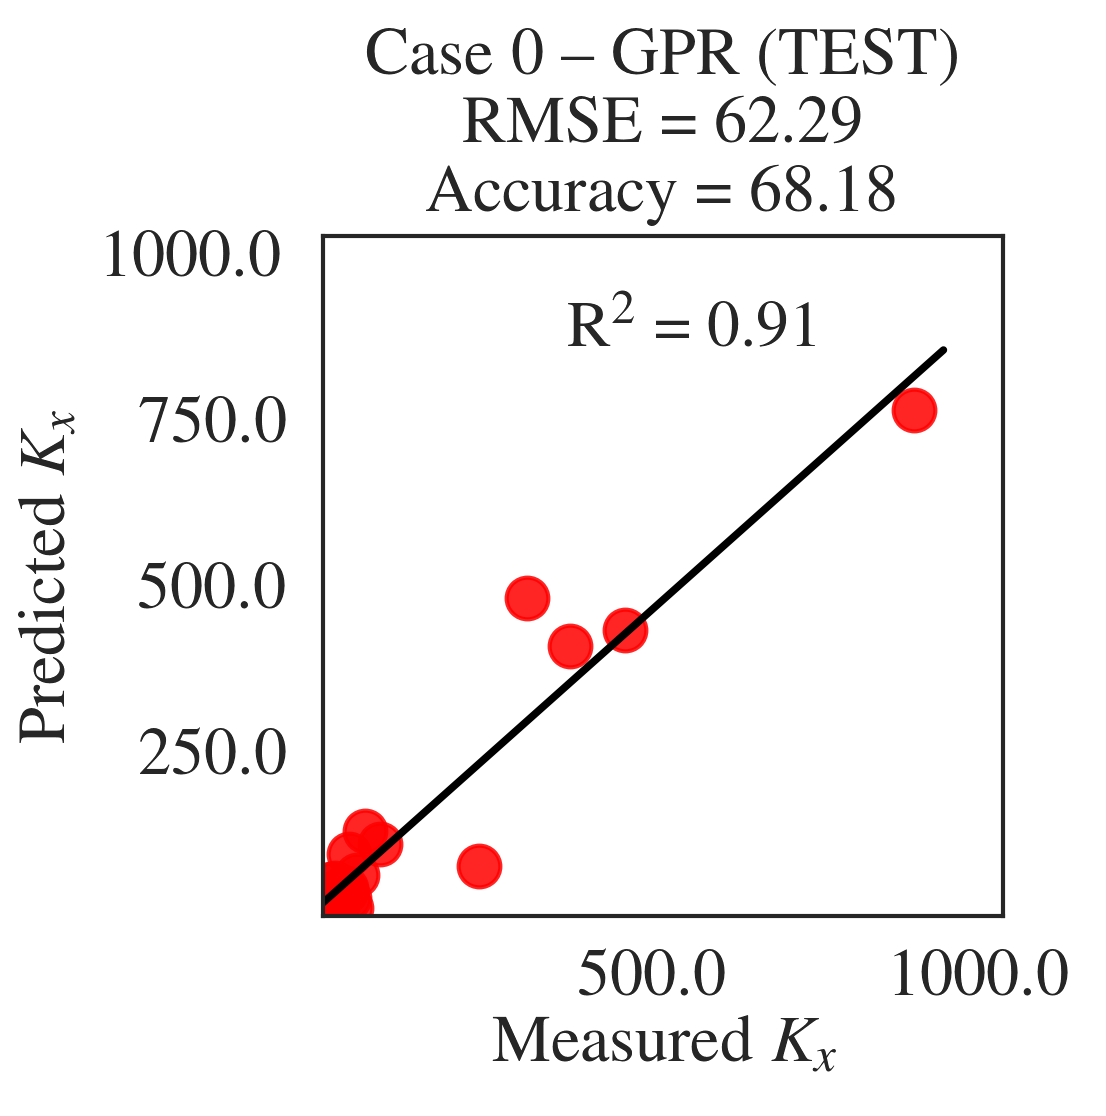
\includegraphics[width=0.3245\textwidth]{./scatter/eml____300dpi_scatter_best_model___gpr__case_0__test}
%  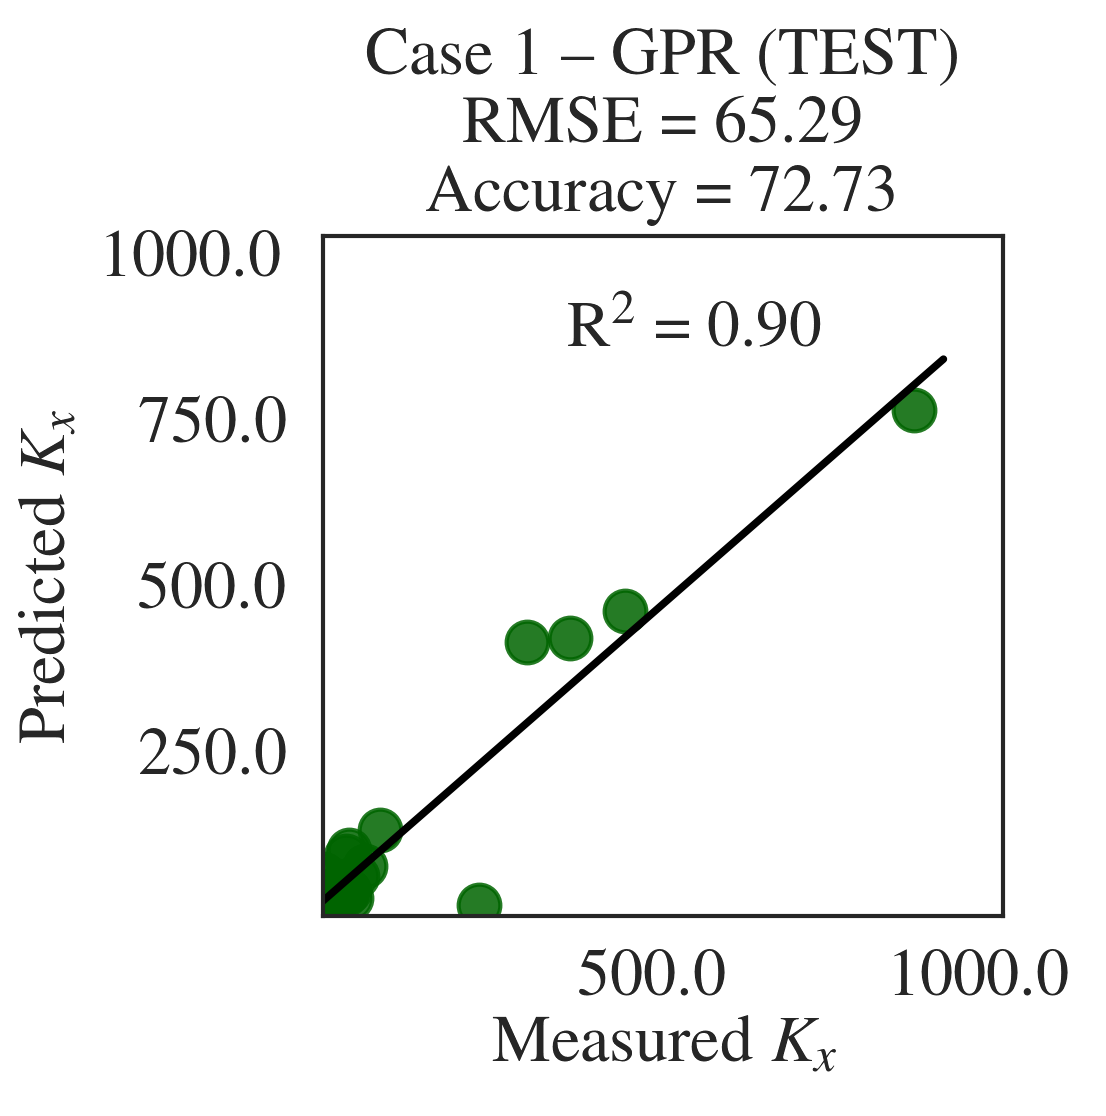
\includegraphics[width=0.3245\textwidth]{./scatter/eml____300dpi_scatter_best_model___gpr__case_1__test}
% 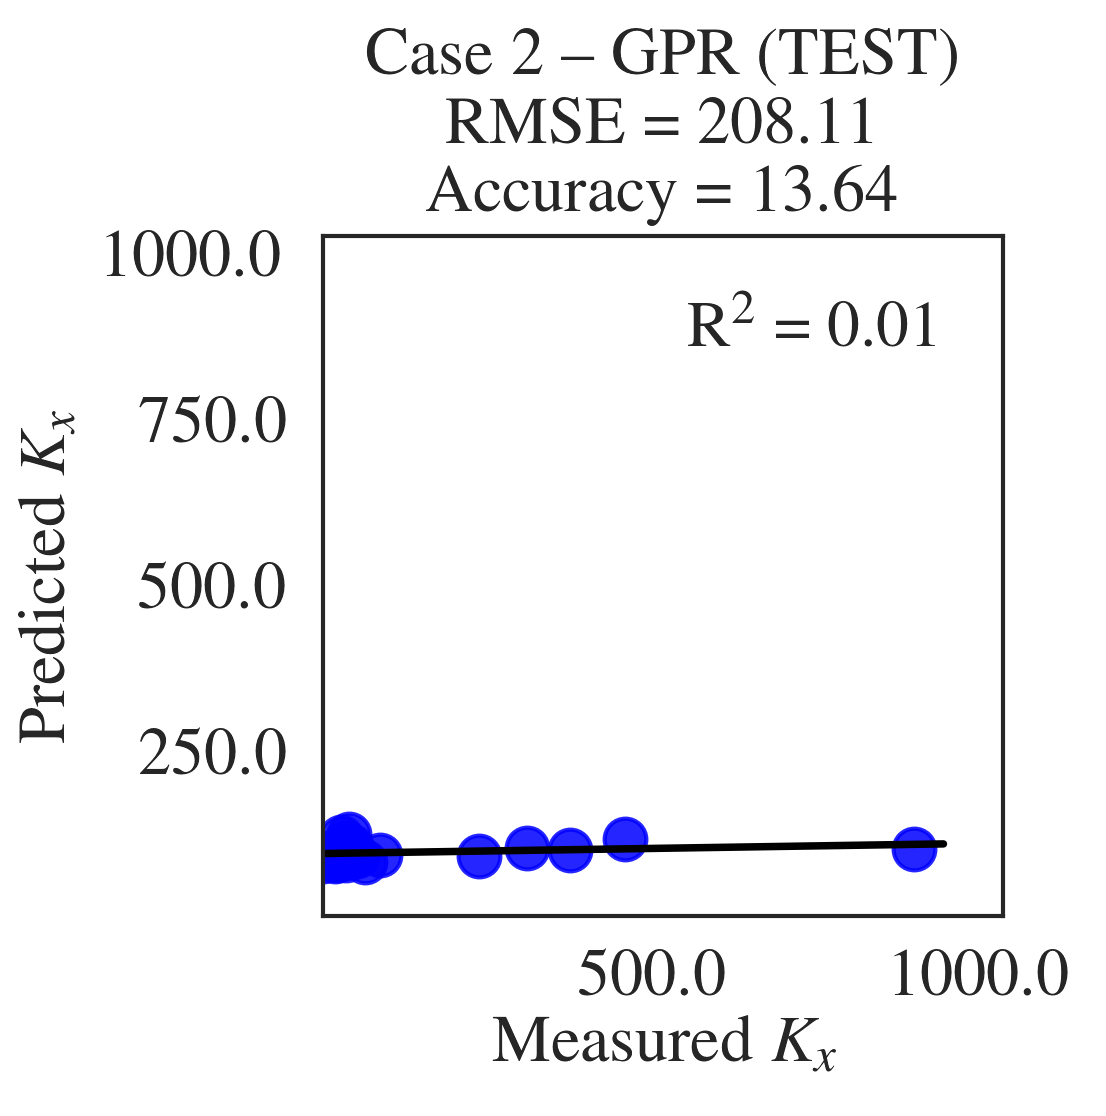
\includegraphics[width=0.3245\textwidth]{./scatter/eml____300dpi_scatter_best_model___gpr__case_2__test}
% 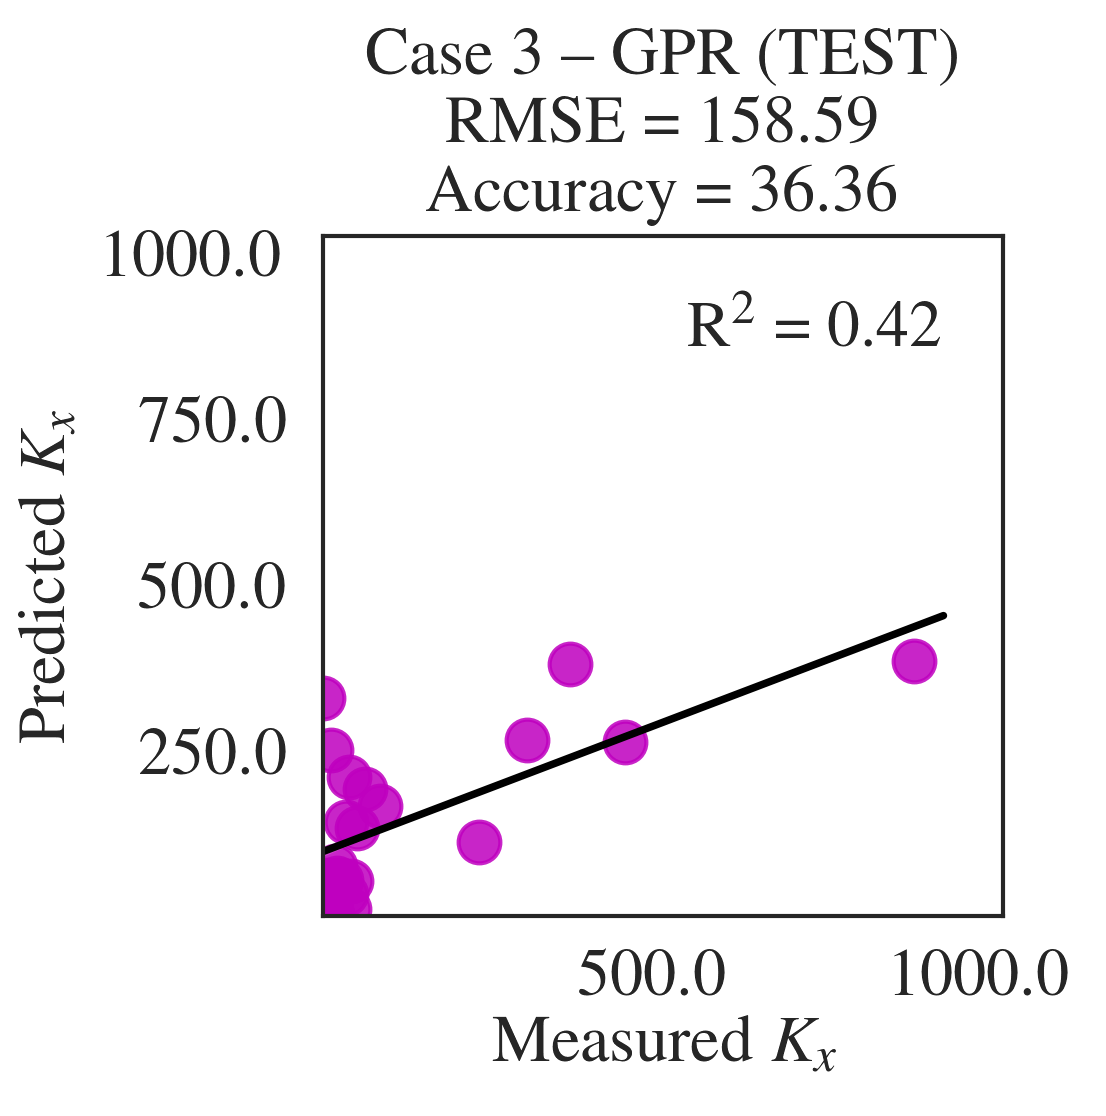
\includegraphics[width=0.3245\textwidth]{./scatter/eml____300dpi_scatter_best_model___gpr__case_3__test}
% 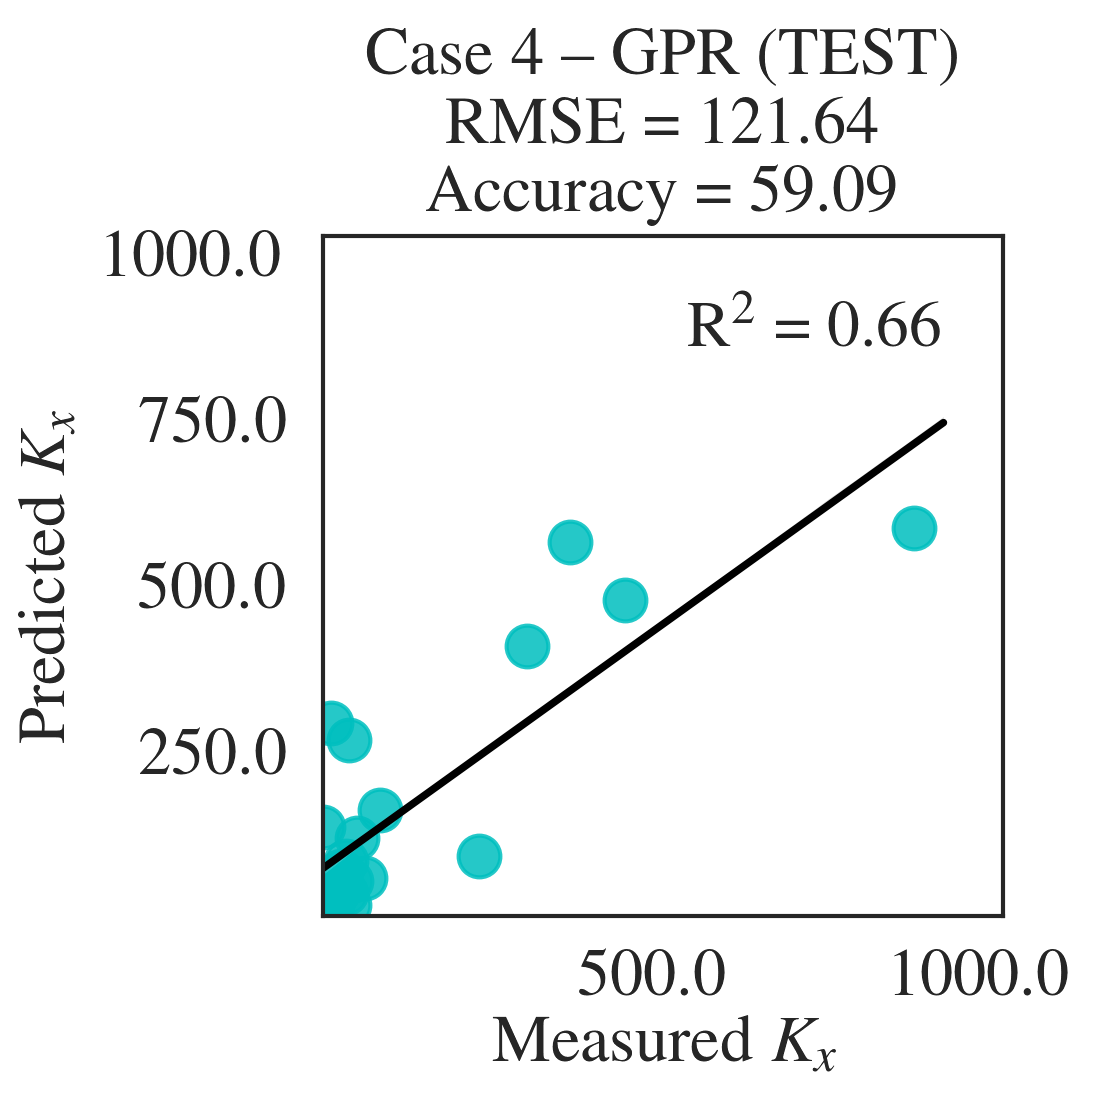
\includegraphics[width=0.3245\textwidth]{./scatter/eml____300dpi_scatter_best_model___gpr__case_4__test}
% 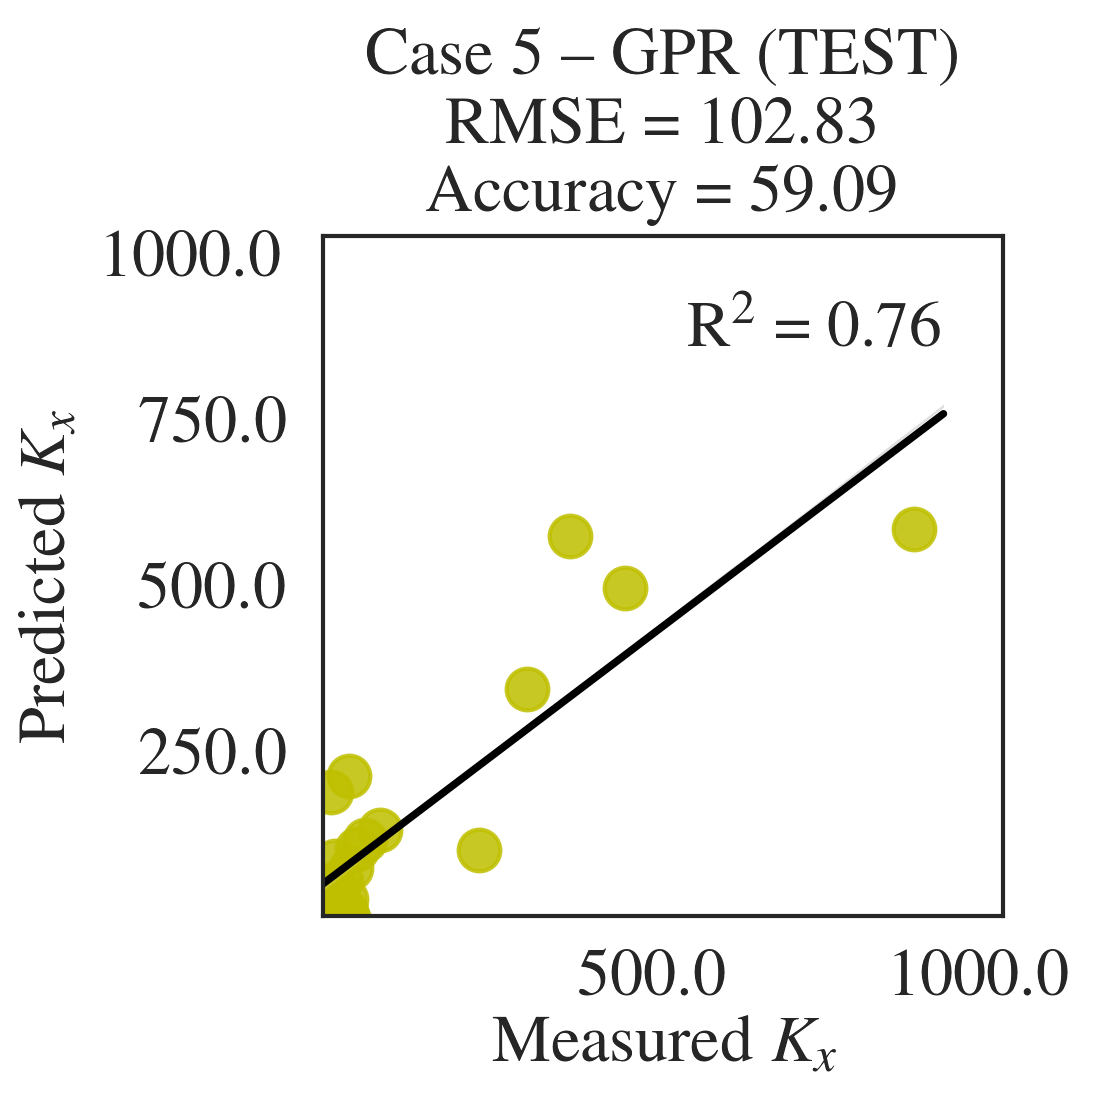
\includegraphics[width=0.3245\textwidth]{./scatter/eml____300dpi_scatter_best_model___gpr__case_5__test}
% 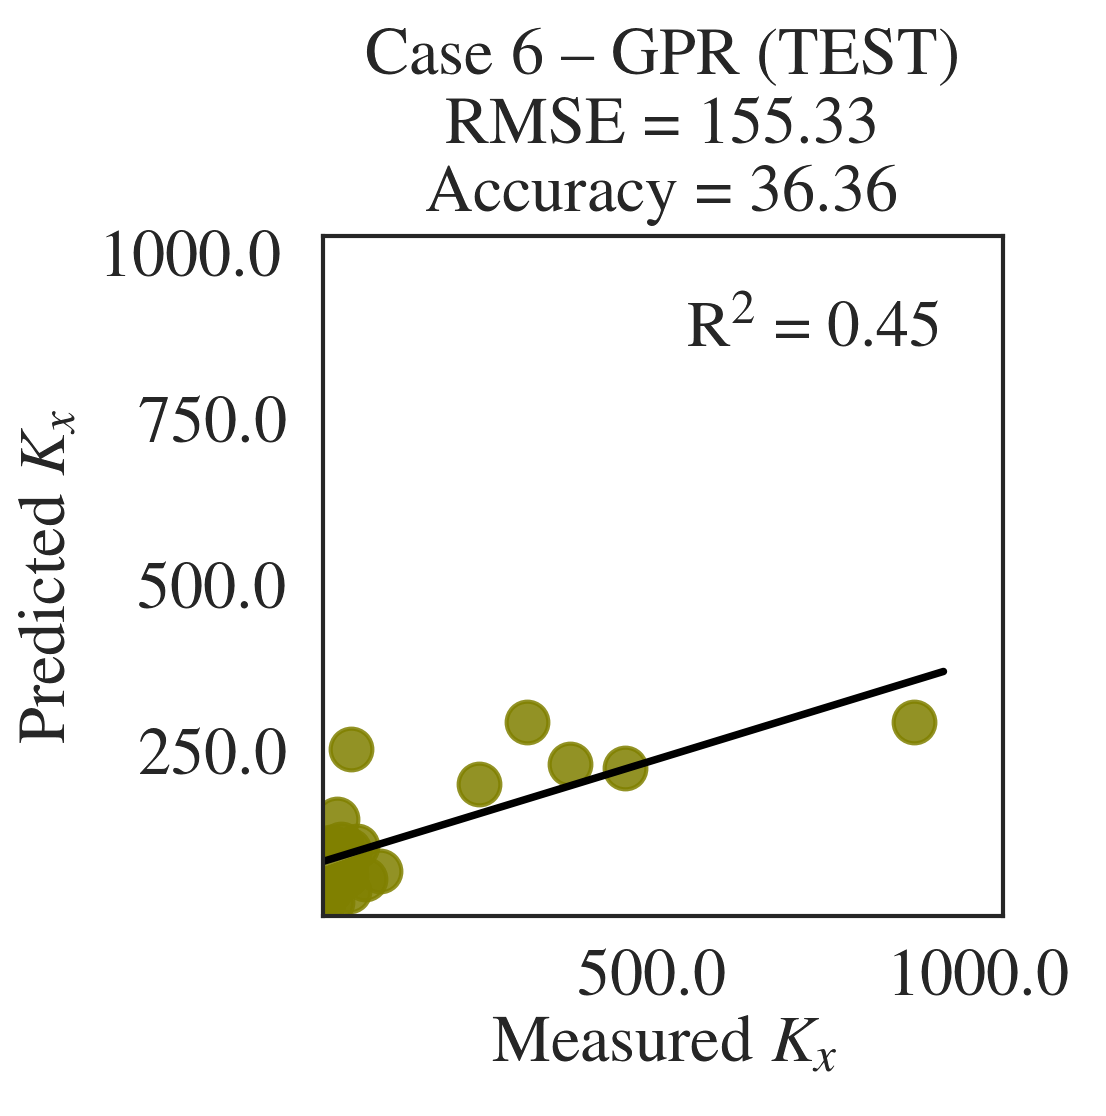
\includegraphics[width=0.3245\textwidth]{./scatter/eml____300dpi_scatter_best_model___gpr__case_6__test}
% 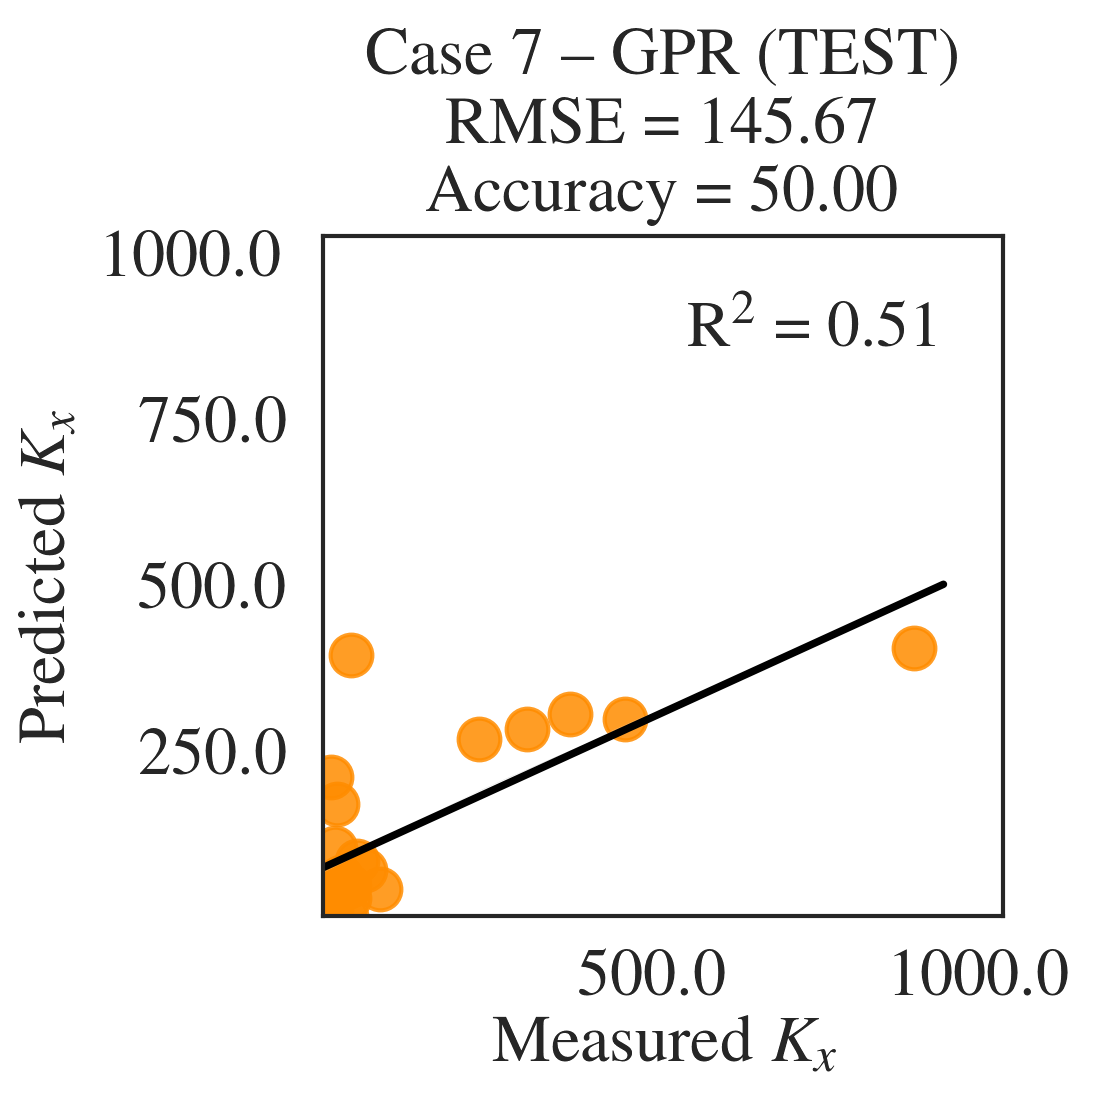
\includegraphics[width=0.3245\textwidth]{./scatter/eml____300dpi_scatter_best_model___gpr__case_7__test}
%  \caption{\label{fig:eml____300dpi_scatter_best_model___gpr__ldc}
%  Scatter plots for the best models according to Root Mean Squared Error (RMSE) using the hybrid model.}
% \end{figure}

% \begin{figure}[!tbp]
%  \centering 
% 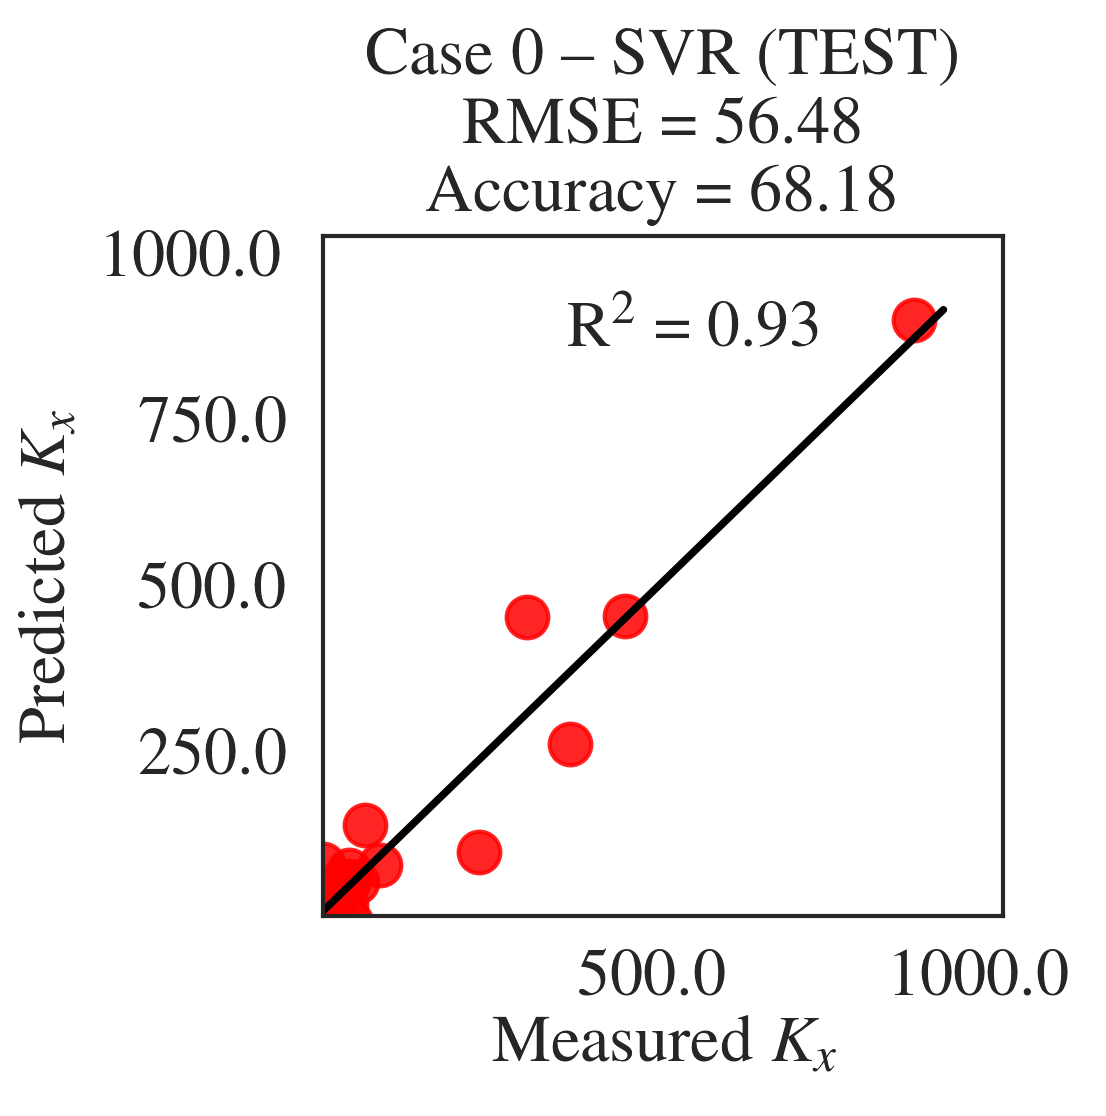
\includegraphics[width=0.3245\textwidth]{./scatter/eml____300dpi_scatter_best_model___svr__case_0__test}
% 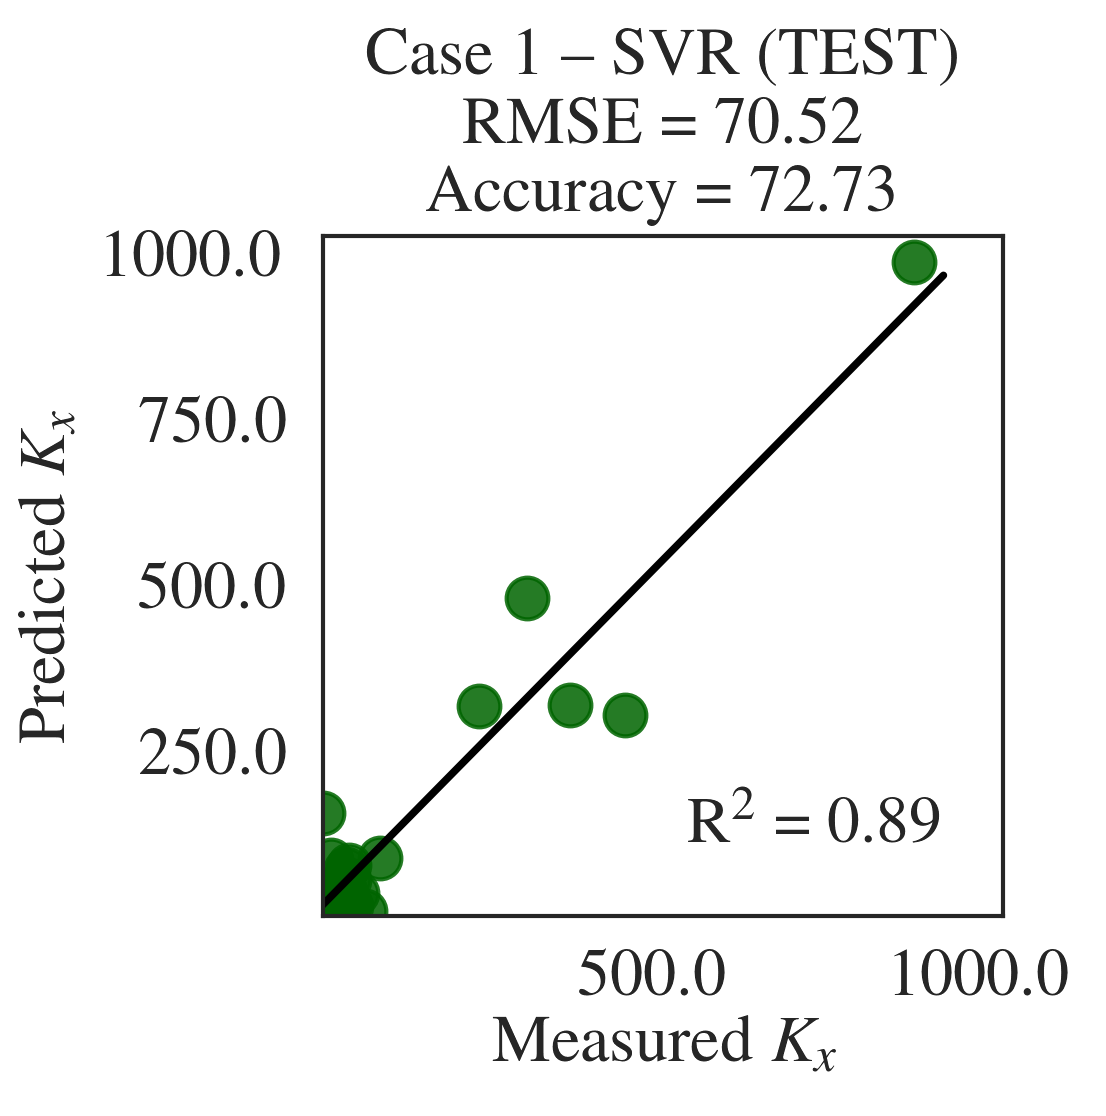
\includegraphics[width=0.3245\textwidth]{./scatter/eml____300dpi_scatter_best_model___svr__case_1__test}
% 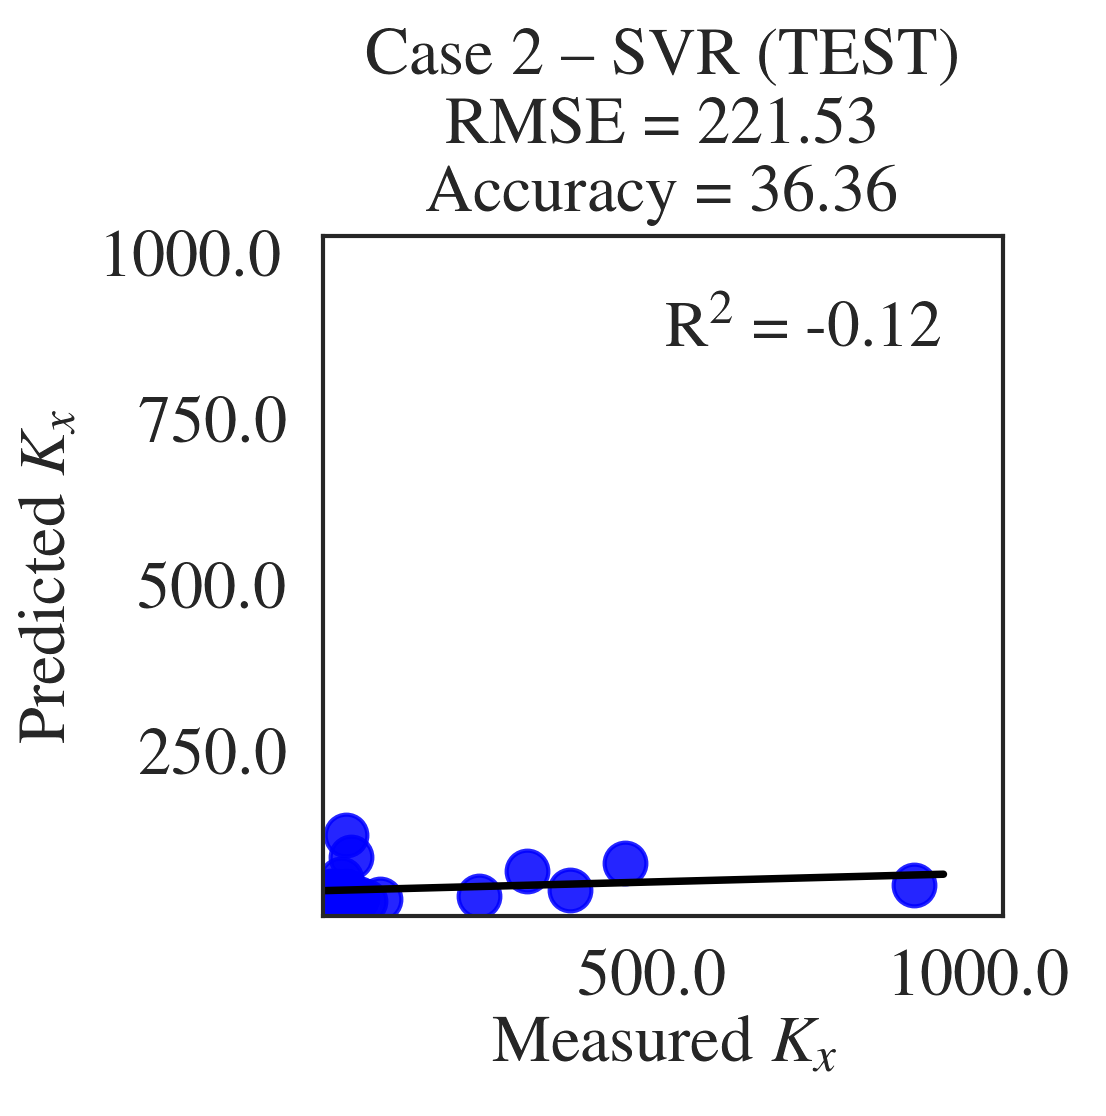
\includegraphics[width=0.3245\textwidth]{./scatter/eml____300dpi_scatter_best_model___svr__case_2__test}
% 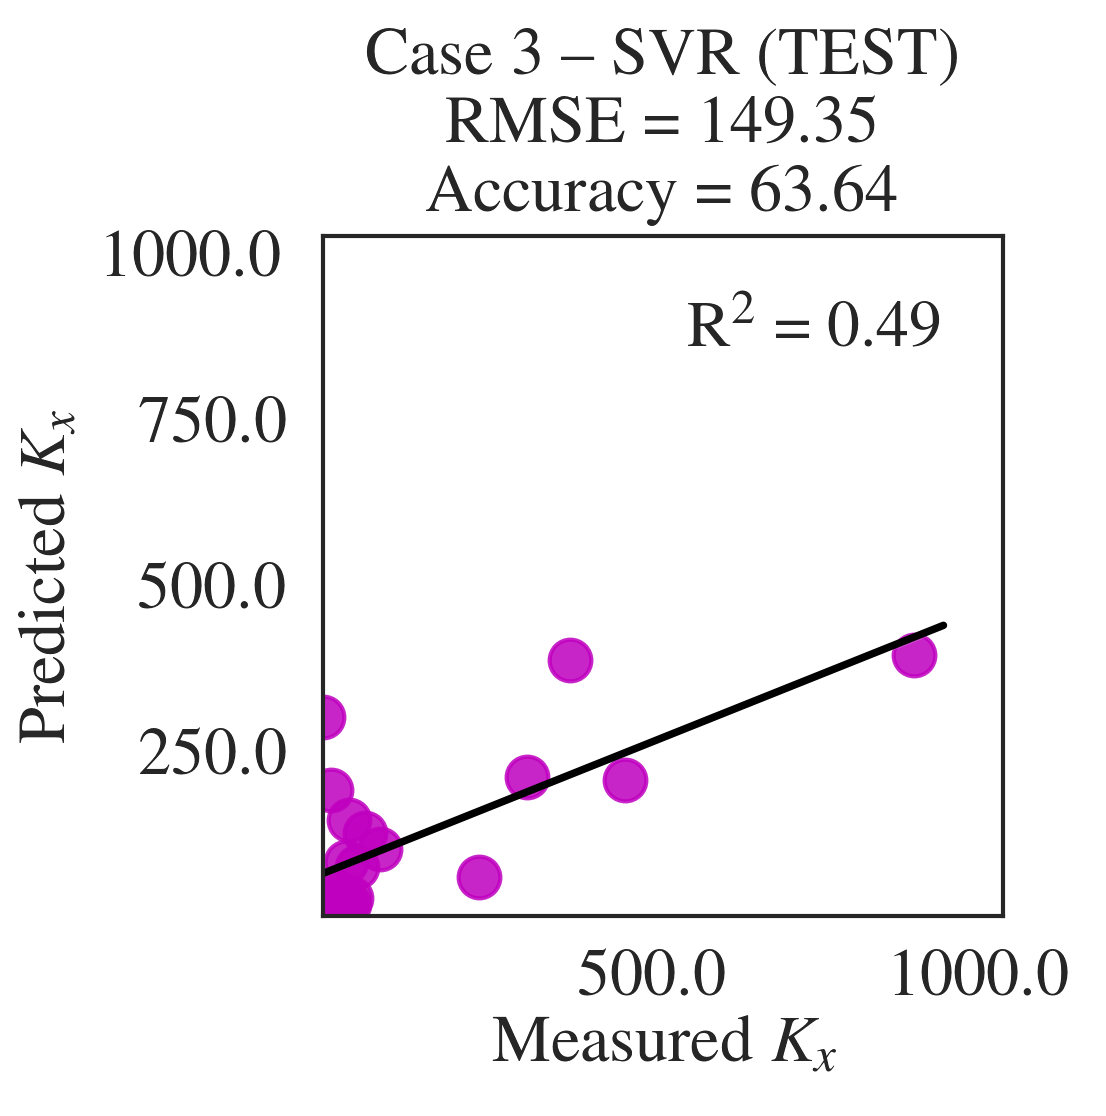
\includegraphics[width=0.3245\textwidth]{./scatter/eml____300dpi_scatter_best_model___svr__case_3__test}
% 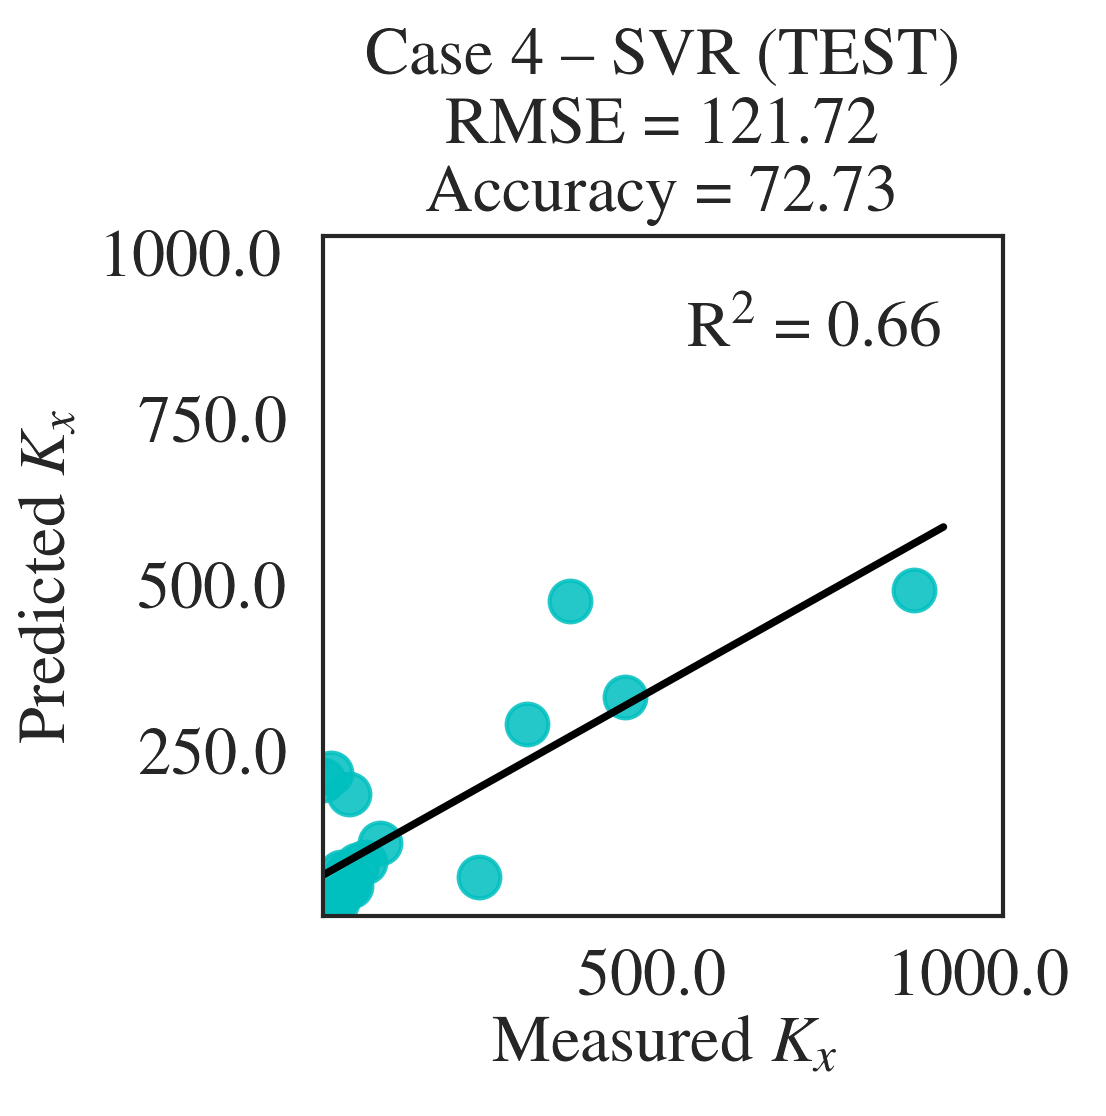
\includegraphics[width=0.3245\textwidth]{./scatter/eml____300dpi_scatter_best_model___svr__case_4__test}
% 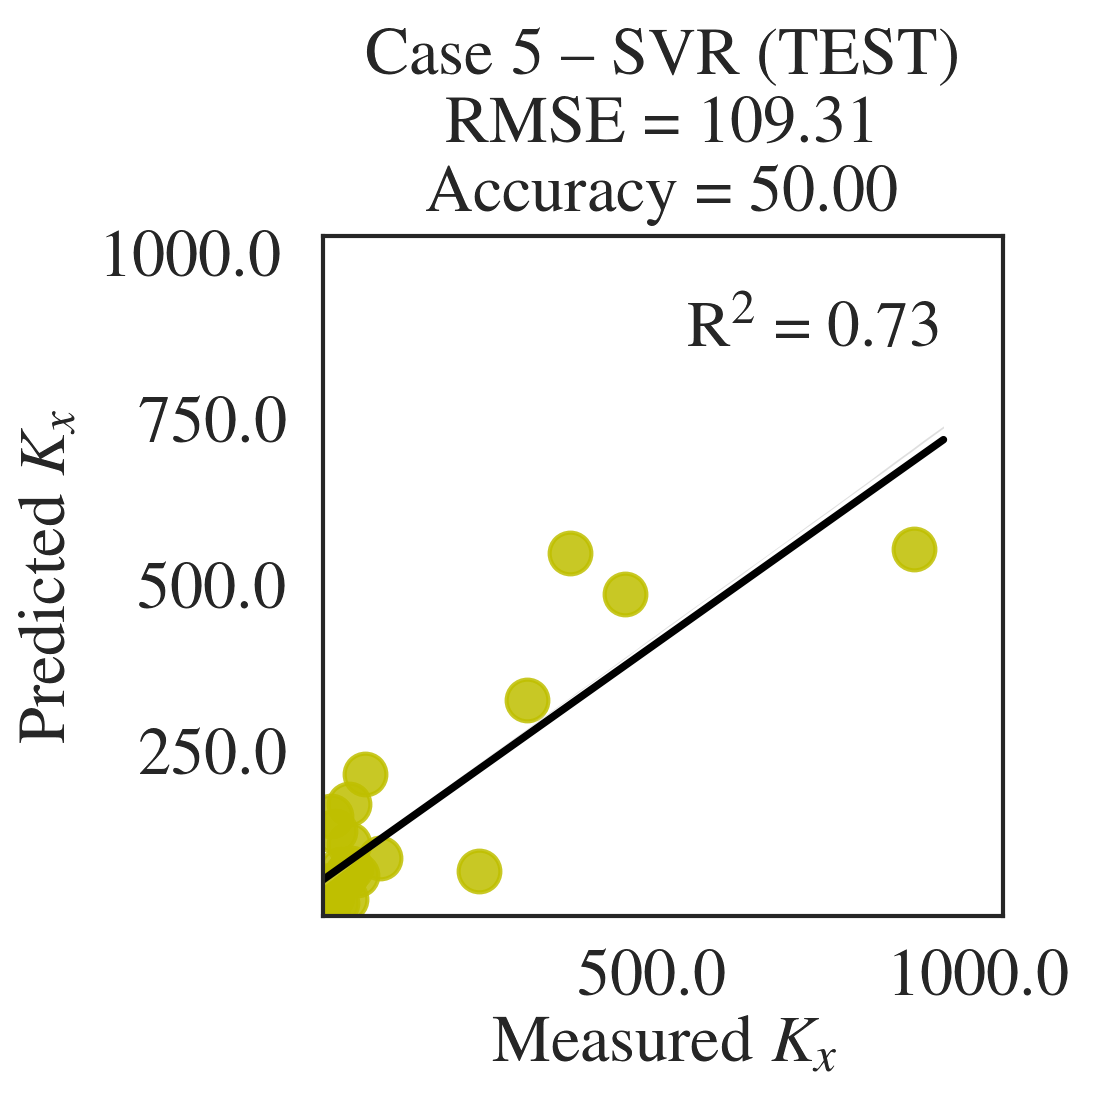
\includegraphics[width=0.3245\textwidth]{./scatter/eml____300dpi_scatter_best_model___svr__case_5__test}
% 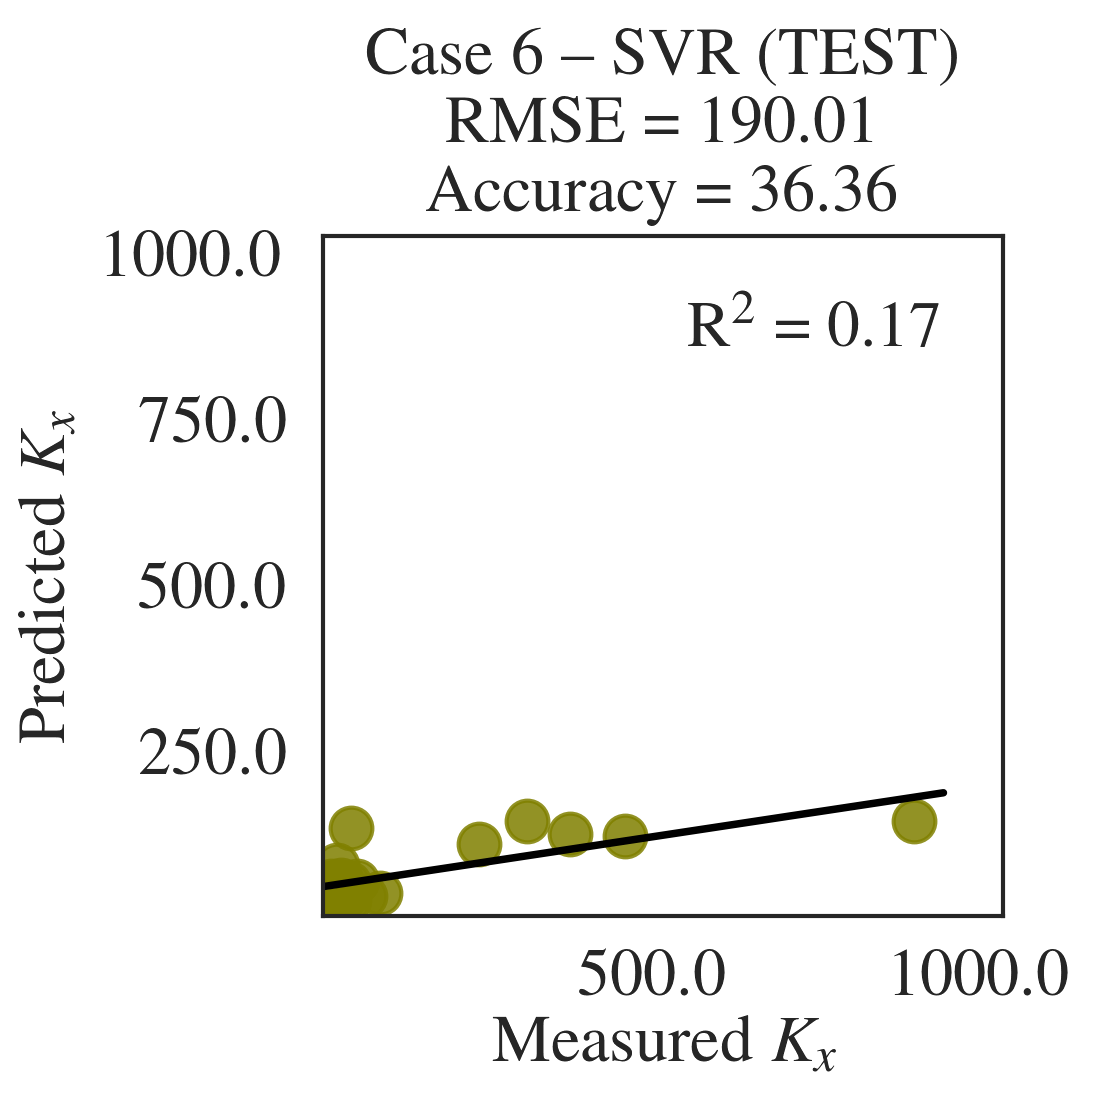
\includegraphics[width=0.3245\textwidth]{./scatter/eml____300dpi_scatter_best_model___svr__case_6__test}
% 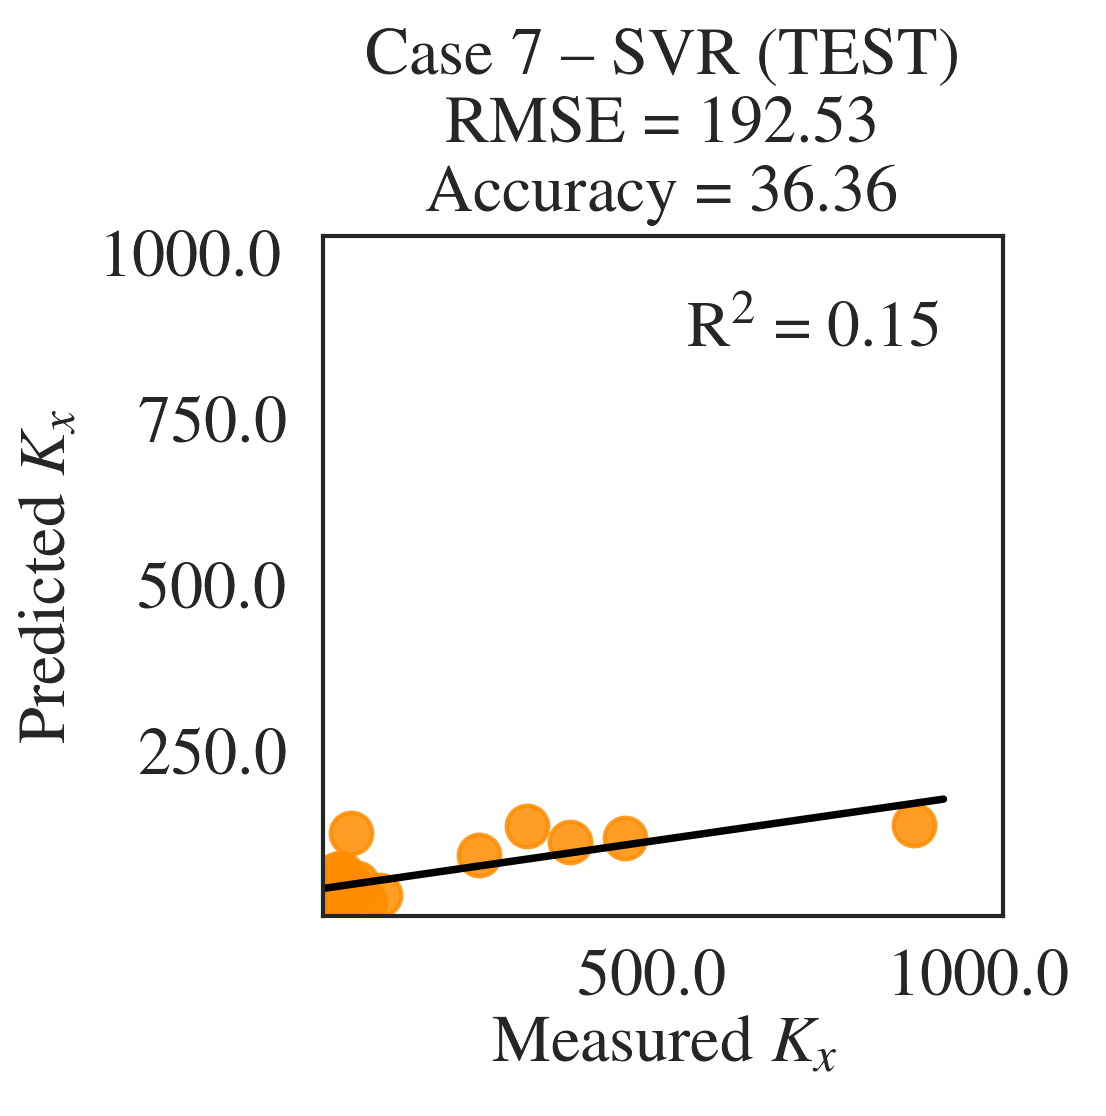
\includegraphics[width=0.3245\textwidth]{./scatter/eml____300dpi_scatter_best_model___svr__case_7__test}
% \caption{\label{fig:eml____300dpi_scatter_best_model___svr__ldc}
% Scatter plots for the best models according to Root Mean Squared Error (RMSE) using the hybrid model.}
% \end{figure}



%---------------------------------------------------------------------------------
\subsection{\label{sec:ldc-efs} Modeling $K_x$ with evolutionary feature selection}
%---------------------------------------------------------------------------------


Considering the experiments in the last section, it is not clear whether other combinations of variables can lead to better results for RMSE and accuracy. Despite the explanation provided by the authors in their study \cite{tayfur2005predicting}, it can be argued that the variables associated with the cases shown in Table \ref{tab:cases-features} were chosen, in their major extent,  based on the correlation with the longitudinal dispersion coefficient. Figures \ref{fig:eml____300dpi_correlation_target___k_x} and \ref{fig:eml____300dpi_scatter_target} show that the variables with the highest correlations are those that comprise the sets in  Table \ref{tab:cases-features}.
For example, the $U$ variable appears in 5 out of 8 cases. Besides, the variables $U$, $B$, and $H$ are part of Cases 1 and 2, which produced the best results.

The hybrid approach developed here can search for the most suitable variables along with the estimator to explore combinations that not previously considered.  It can be noticed that due to the nonlinear natures of the estimators GPR and SVR,
a careful choice of variables can produce an improved performance of the estimators. Moreover, variables with smalls correlations with $K_x$ may positively impact the final predictions. The next experiments aim at analyzing the impact of the evolutionary feature selection on the assessment of the performance metrics on the $K_x$ prediction.


% 
\begin{table}[!htb]
\centering
\caption{\label{tab:results_fs}  
Hybrid evolutionary approach with feature selection.
The best results are shown in boldface with standard deviation in parentheses. Values indicated with  -- were not available at the source.
}
\begin{tabular}{rrrrrr}
\hline
Case      & Estimator &                 RMSE &           Accuracy   &    RMSE$(K_x<100)$ &       RMSE$(B/H<50)$    \\\hline                                                               
%    Case 0 &       REF &          193.00 (--) &           70.00 (--) &  { \bf 19.30} (--) &          183.00 (--)  \\
%    Case 1 &       REF &         193.00  (--) &         75.00  (--)  &        21.20  (--) &         183.00  (--)  \\
   Case 0 &       GPR &         99.70  (29.05) &         67.91 (5.05)&       31.80 (3.97) &          63.13 (10.63) \\
          &       SVR &         112.34 (26.40) &         57.73 (7.06)&       41.23 (4.28) &         58.80 (7.58)   \\
          &       REF &            193.00 (--) &    {     70.00} (--)&  { \bf 19.30} (--) &            183.00 (--) \\\\
   Case 1 &       GPR &        167.34 (115.45) &         71.05 (6.19)&       41.28 (8.16) &         114.68 (98.36) \\
          &       SVR &        113.22  (35.35) &         62.59 (5.96)&       45.18 (8.84) &          61.73 (14.43) \\
          &       REF &            193.00 (--) &     {    75.00} (--)&  {     21.20} (--) &            183.00 (--) \\\\
   --     &    GPR-FS &   { \bf 83.26} (26.41) & { \bf 76.73} (6.60) &       31.25 (5.18) &        52.41 (14.61)   \\
   --     &    SVR-FS &          88.78 (13.66) &        65.77 (8.99) &       39.51 (8.42) &    { \bf 46.10} (7.21) \\
%  Case 2 &       REF &         191.00  (--) &         65.00  (--) &        20.00  (--) &         179.00  (--) \\
%  Case 3 &       REF &         170.00  (--) &         40.00  (--) &       146.00  (--) &         164.00  (--) \\
%  Case 4 &       REF &         137.00  (--) &         70.00  (--) &       105.00  (--) &         118.00  (--) \\
%  Case 5 &       REF &         119.00  (--) &         58.00  (--) &        77.70  (--) &          99.00  (--) \\
%  Case 6 &       REF &         159.00  (--) &         50.00  (--) &       104.30  (--) &          42.00  (--) \\
%  Case 7 &       REF &         142.00  (--) &         58.00  (--) &        93.80  (--) &          67.00  (--) \\
\hline 
\end{tabular} 
\end{table}

Table \ref{tab:results_fs} summarized the results obtained for GPR and SVR assitsed by feature selection in the pipeline shown in Figure \ref{fig:framework}.
The first column shows the cases, and the second column displays the estimator. The Root Mean Squared Error is shown in the third column, while the Accuracy appears in the fourth column. The fifth two columns show the Root Mean Squared Error when extreme values are discarded and the last one the RMSE for narrow channels.
% 
Analyzing the results in Table  \ref{tab:results_fs}, it is possible to observe that the feature selection step on the pipeline has contributed considerably to improve the metrics produced by the machine learning methods. Table \ref{tab:results_fs} also shows the results for Cases 1 and 2 to compare the performance of the models when the feature selection was not applied.
% 
Overall, the RMSE values decreased for both GPR and SVR models. 
As observed for the models without implementing feature selection, GPR-FS and SVR-FS produced smaller Root Mean Squared Errors than the reference model.
GPR-FS model achieved, on average, an improvement of 16.5\% when compared to Case 0 and 50.2\% concerning Case 1. The improvement achieved by the model SVR-FS to Cases 0 and 1 were 21.0\% and 21.6\%, respectively.

Regarding Accuracy, the SVR-FS model achieved a slight improvement over the SVR model. On the other hand, the GPR-FS model achieved a consistent improvement when compared to the model without feature selection. In particular, the averaged Accuracy is the highest among all models.
% 
When the extreme dispersion coefficients ($ K_x> 100 $) were excluded, there was no improvement in the RMSE for both methods. However, the evolutionary pipeline implementing  GPR and SVR models allowed us to reach the lowest RMSE values for narrow channels. In particular, the average values of RMSE achieved by the SVF-FS model can be highlighted, as can be seen in the last column of Table  \ref{tab:results_fs}.
% 
Figure \ref{fig:eml____300dpi_scatter_best_model_fs___ldc} depicts the scatter plots for the best GPR-FS and SVR-FS models, that were chosen according to the smaller RMSE.
Considering GPR-FS, 
it can be observed that RMSE deacreased while Accuracy increased
when comparing the scatter plots from Figures
\ref{fig:eml____300dpi_scatter_best_model___ldc}
and 
\ref{fig:eml____300dpi_scatter_best_model_fs___ldc}.

\begin{figure}[!htb] \centering 
 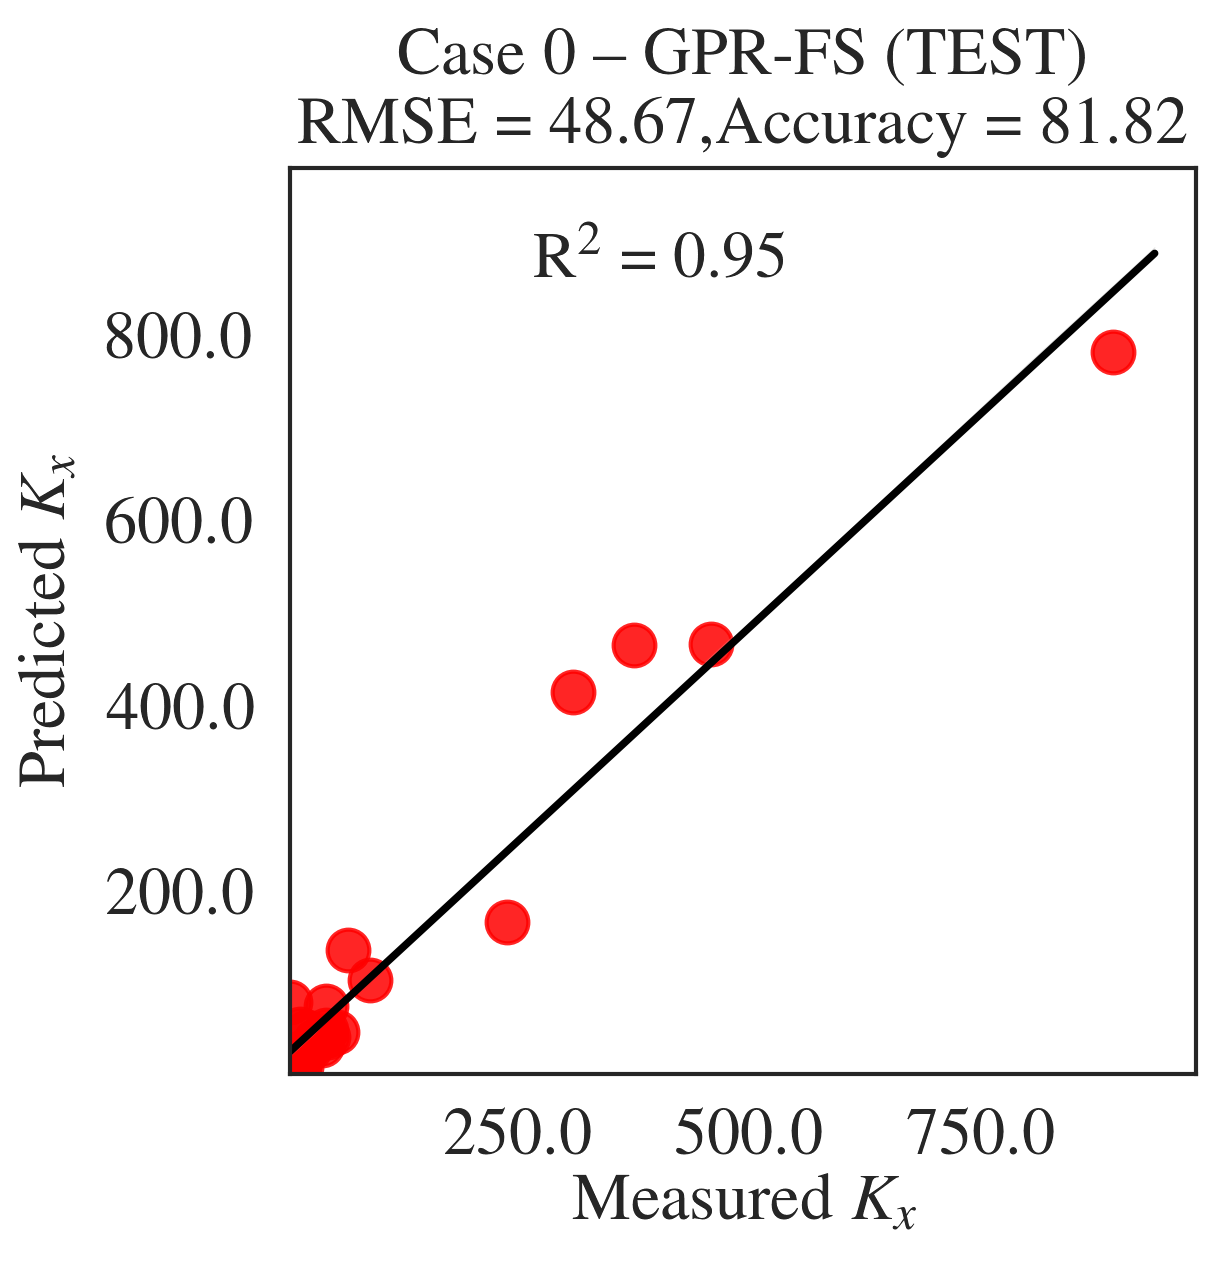
\includegraphics[width=0.33245\textwidth]{./scatter/eml____300dpi_scatter_best_model___gpr_fs__case_0__test}
 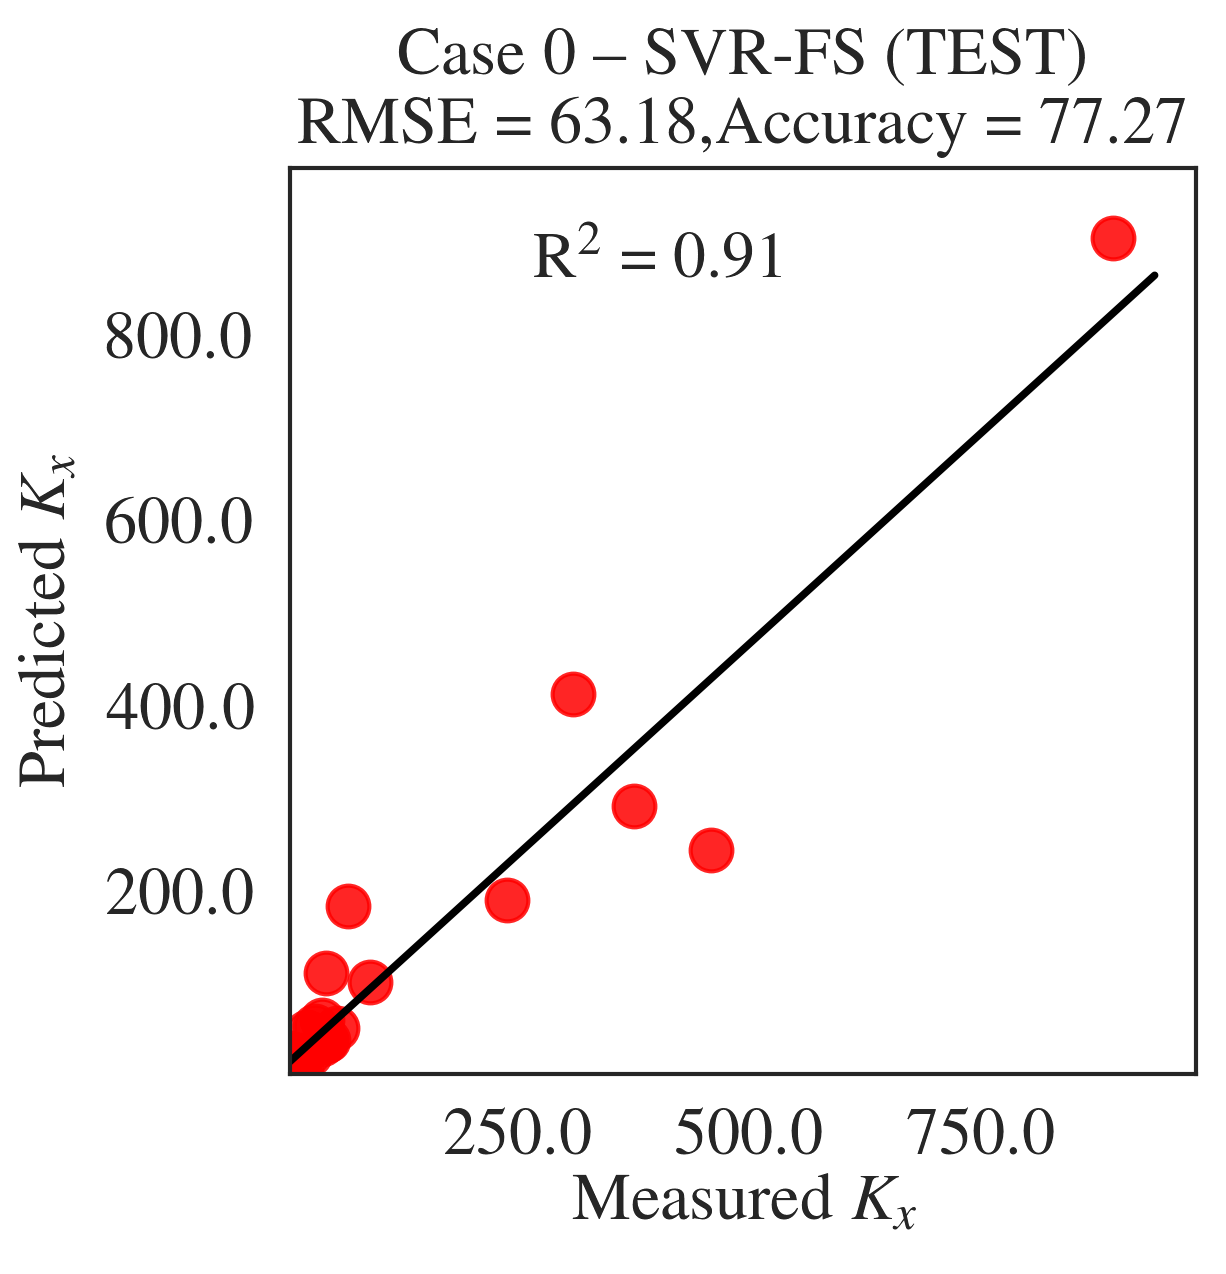
\includegraphics[width=0.33245\textwidth]{./scatter/eml____300dpi_scatter_best_model___svr_fs__case_0__test}
 \caption{\label{fig:eml____300dpi_scatter_best_model_fs___ldc}
 Scatter plots for the best models implementing evolutionary feature selection according to Root Mean Squared Error (RMSE).}
\end{figure}

The analysis of these results allows us to conclude that the feature selection step in the pipeline leads to a considerable improvement in the prediction of the dispersion coefficient. The proper selection of input variables is beneficial for the pipeline model as this interaction increases the accuracy while decreases the averaged errors.

The results reported in Table \ref{tab:results_fs} allow us to assess the improvement in performance, but they do not show which variables led to these gains. Figure \ref{fig:eml____300dpi_active_features_sets_count} shows the distribution of the selected features after training the evolutionary pipeline.
From this figure, one can observe that GPF-FS and SVR-FS chose a total of 13 sets of features at the end of the evolutionary search procedure. We observed the variable selection process is heuristic and there is no guarantee of choosing the same set of variables in all runs.
% 
The barplot on the left side shows that for  GPR-FS model, the set of variables $ B, U, \sigma, Q $ has been selected 24 times, the  $ B, U, \sigma $ was selected 18 times and  $ B, U, \sigma, \beta $ 13 times. These three sets were selected 55 out of 100 times, and they share the variables $ B, U $ and $ \sigma $.
A similar analysis for the SVR-FS model in the bar graph of Figure \ref{fig:eml____300dpi_active_features_sets_count} shows that $ B, U, \sigma, \beta $ was chosen 33 times,  $ B, U, \sigma $ 20 times, and $ B, U, \sigma $ 12 times. These three sets were selected 74 times over the course of 100 independent executions, approximately two thirds of the total runs.
% 
\begin{figure}[!htb]
    \centering 
    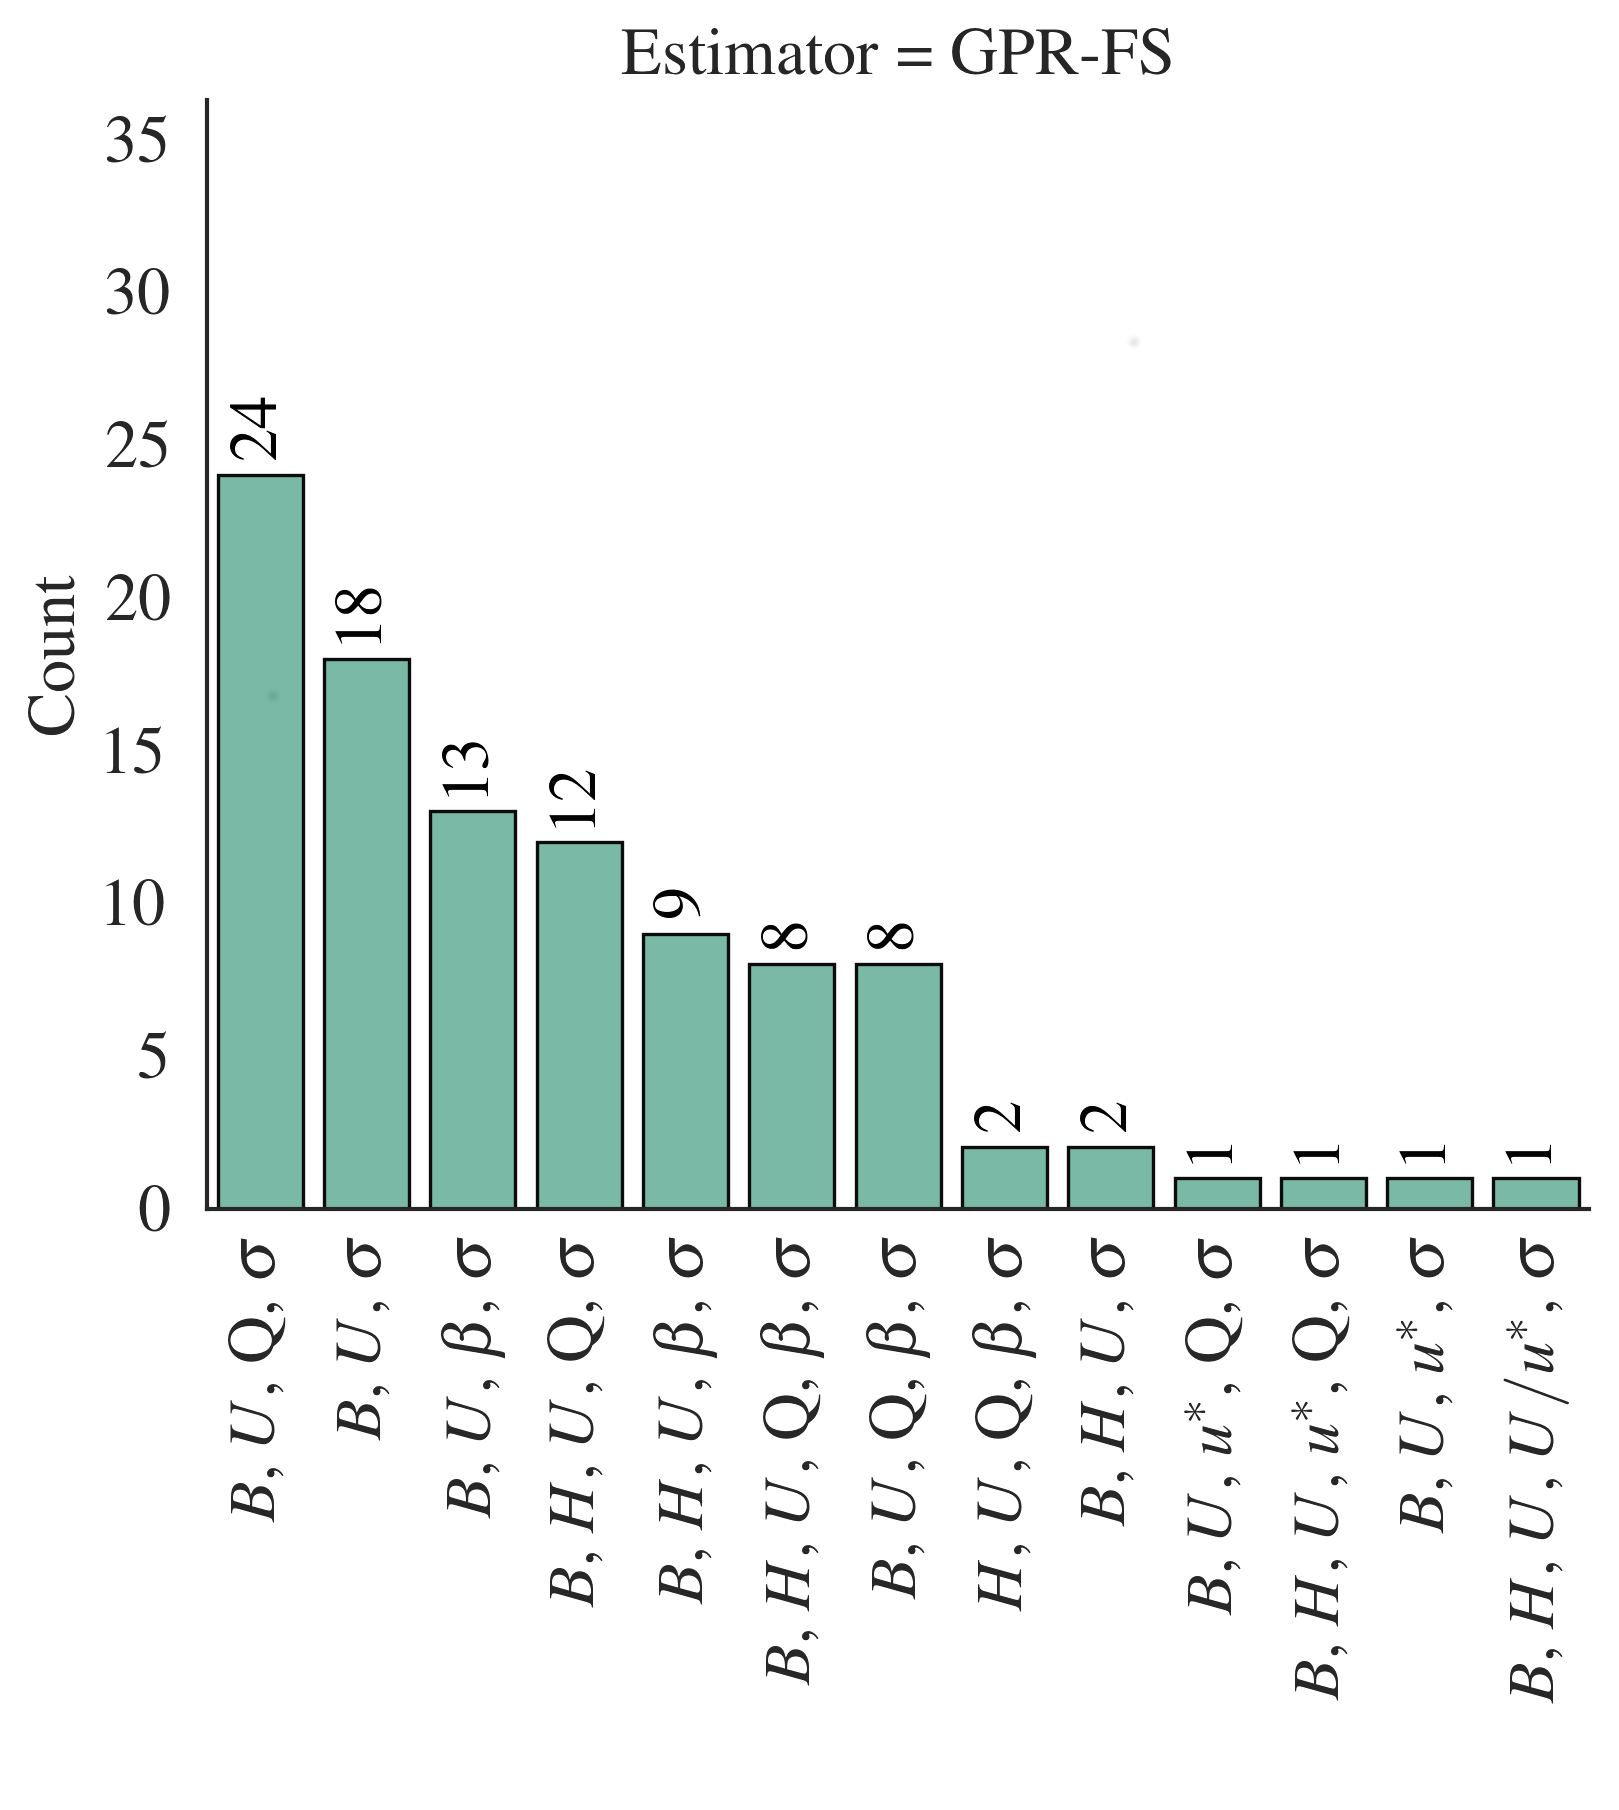
\includegraphics[height=0.41\textheight]{./results/eml____300dpi_active_features_sets_gpr_fs__count}
    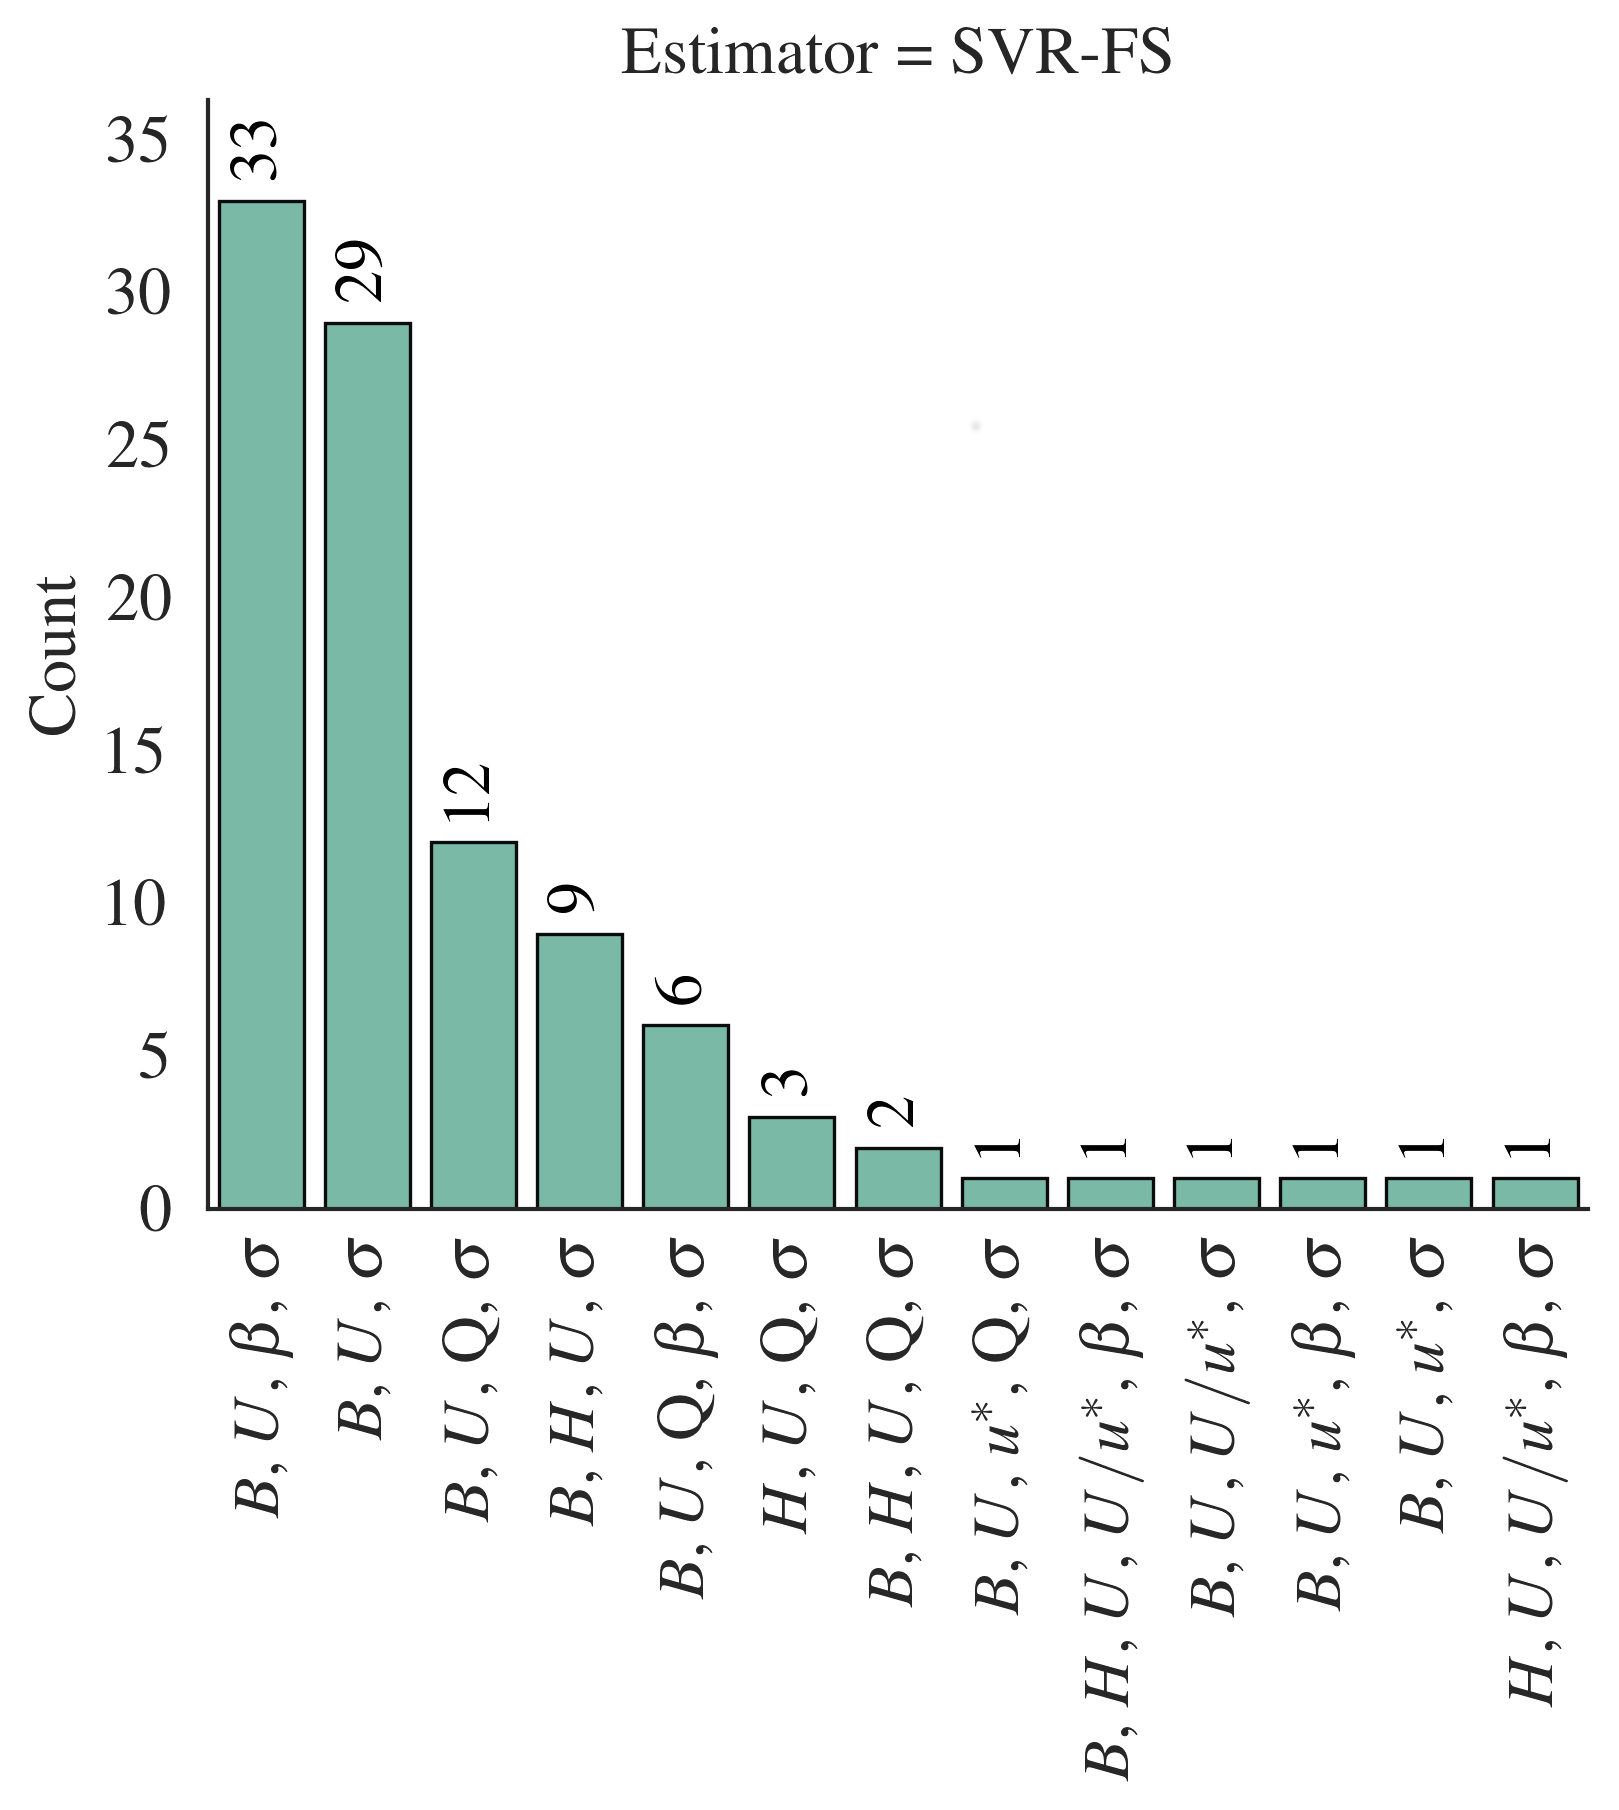
\includegraphics[height=0.41\textheight]{./results/eml____300dpi_active_features_sets_svr_fs__count}
    \caption{\label{fig:eml____300dpi_active_features_sets_count}
    Distribution of sets of  active features for evolutionary feature selection approach over 100 runs.}
\end{figure} 

Figure \ref{fig:eml____300dpi_active_features_distribution__count} shows that $ U, \sigma, B, Q $ were the most frequent variables for the GPR-FS model, in that order. For the SVR-FS model, the most frequent ones were $ U, \sigma, B, \beta $, in this order as well.
Moreover, for both models, the variables $ U $ and $ \sigma $ were select in all runs, while  $ B $  appears 98 times for the GPR-FS model and 96 times for the SVR-FS model.
From most frequent variables, $ U $ and $ B $ have a strong correlation with the dispersion coefficient, whereas river sinuosity $ \sigma $ has the lowest correlation, as can be seen in Figure \ref{fig:eml____300dpi_active_features_distribution__count}. 
% 
The feature selection has shown the sinuosity plays an important rule in the context of the machine learning pipeline. 
In addition, the correlation analysis in Figure 
\ref{fig:eml____300dpi_correlation_target___k_x}
suggests that $\sigma$ holds a strong non-linear relationship with $K_x$. 


Some studies discuss that sinuosity is related to river meandering \cite{deng2002longitudinal} other  exogenous factors such as vegetation \cite{camporeale:2010, savickis:2016} and topography \cite{timar:2003, dijk2013sinuosity}, that also affect the dispersion coefficient.
As shown in the results, the incorporation of sinuosity is  beneficial for the performance of the gaussian processes and support vector machines.



%---------------------------------------------------------------------------------
\subsection{\label{sec:ldc-sfs} Modeling $K_x$ using the most frequent features found by evolutionary selection}
%---------------------------------------------------------------------------------

The computational experiments carried out in this study allow us to determine the importance of variables indirectly. This importance takes into account their impact on the machine learning pipeline.
The results shown in Table  \ref{tab:results_fs} and  Figure \ref{fig:eml____300dpi_active_features_sets_count} suggest that some variables constitute the core that improves the learning of the machine learning models.
A detailed analysis of the frequency that the variables appear in the selected sets is presented in Figure \ref{fig:eml____300dpi_active_features_distribution__count}.
Observing this figure, it is possible to verify that the variable $ \sigma $ appears in all selected sets. The same occurs with the variable $ U $. 
% 
Based on this analysis,  we can see that the most frequent features are $U, B$, and $\sigma$. These three variables are used to propose the Case 8 are shown in Table \ref{tab:results_fs}. 
% Case 9 is made up of the three most frequent ones, $U, B, \sigma$ and $Q$.
% $\beta$ was not included in Case 9, since  the a statistical analysis the the features shows
% a correlation equals to 0.94 between $Q$ and $\beta$.

\begin{figure}[!htb]
    \centering 
    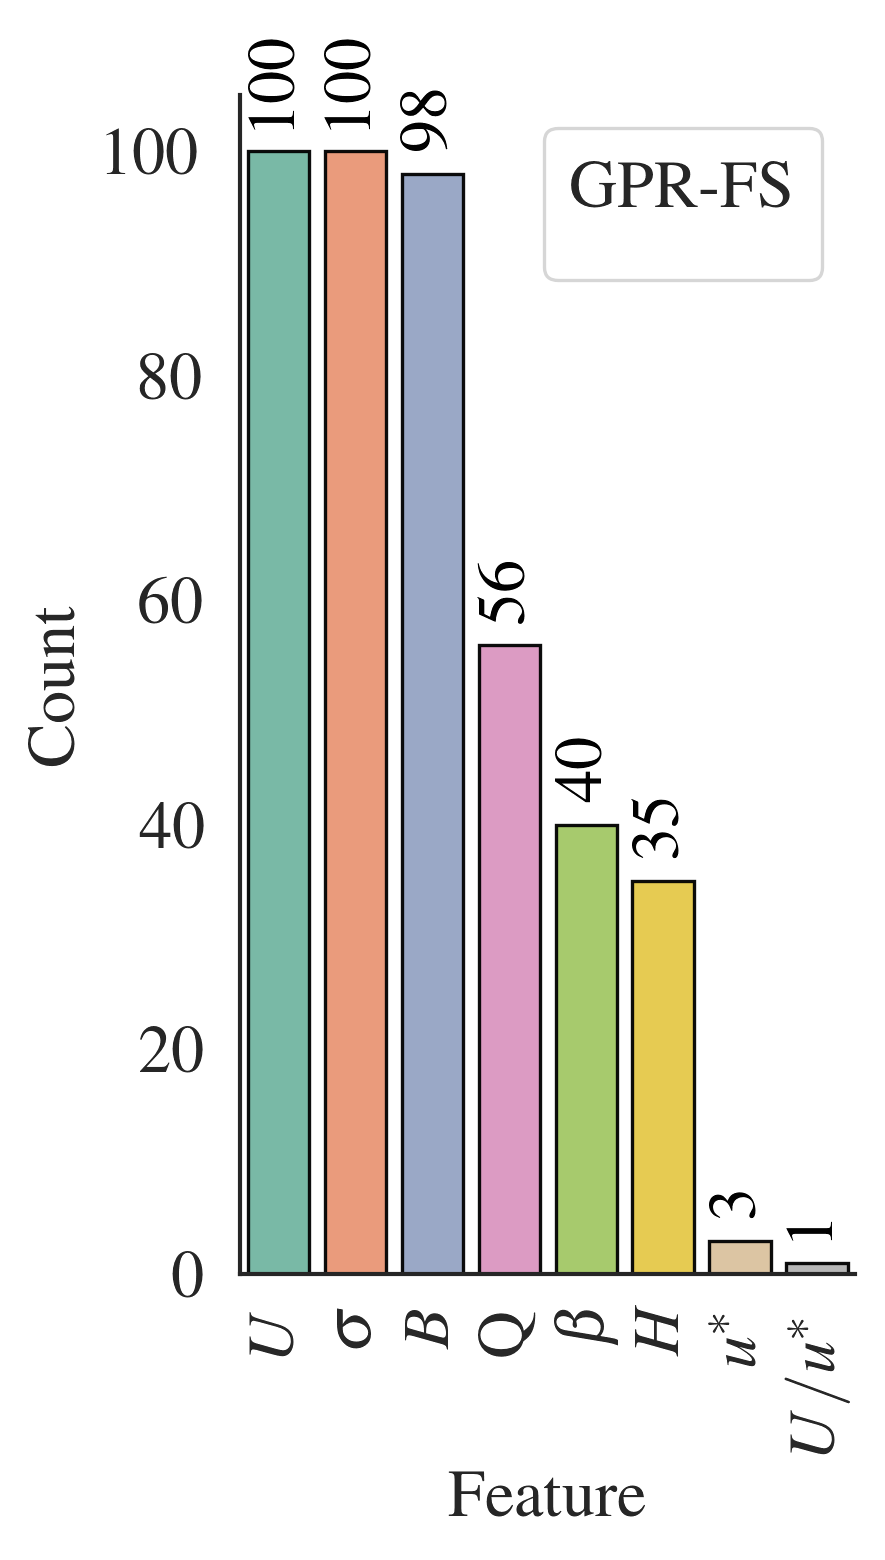
\includegraphics[height=0.35\textheight]{./results/eml____300dpi_active_features_distribution_gpr_fs__count}
    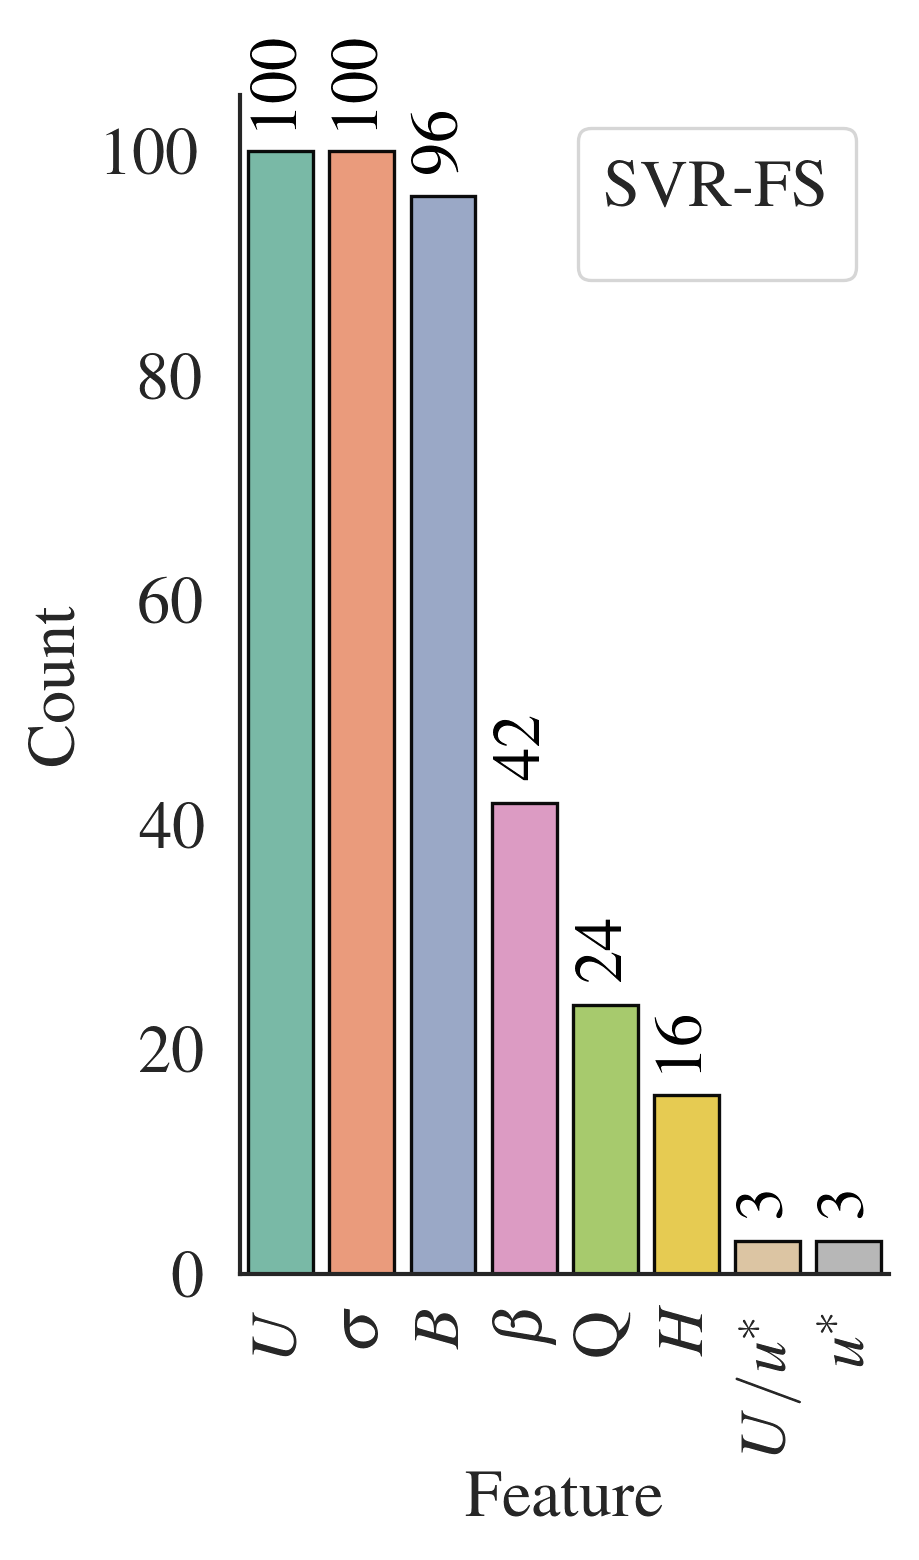
\includegraphics[height=0.35\textheight]{./results/eml____300dpi_active_features_distribution_svr_fs__count}
    \caption{\label{fig:eml____300dpi_active_features_distribution__count}
    Hybrid model using evolutionary feature selection approach.
    Number of times each variable appears in the active sets  over 100 runs.}
\end{figure}


\begin{table}[!htb]
    \centering
    \caption{ \label{tab:cases-features-fs} Feature sets suggested by the analysis of evolutonary feature selection.
    }
    \begin{tabular}{ccl}
    \hline
        Case   & $\xfs$ & Active variables                             \\ \hline
        Case 8 &  10100001  & $U ,     B,                      \sigma$    \\ \hline
%         Case 9 &  10101001  & $U ,     B,      Q,              \sigma$    \\ 
\end{tabular}
\end{table}

A set of computational experiments have been conducted on the Case 8, 
where the the machine learning methods were trained using the  features  $U, B$, and $\sigma$.
The results in Table \ref{tab:results_new_set} shows the improvement of all metrics. 
The averaged values produced for all metrics shows the improvement for GPR  concerning the Root Mean Squared Error, Accuracy and RMSE for dispersion coefficients below 100 m$^2$/s.
% 
This expected because the carefully choosing process of the most frequent variables  represents the indirect introduction of specific knowledge about the features. 
In addition, this specific knowledge could only be obtained after analyzing the various simulations carried out with the evolutionary selection model.
The most frequent variables allow capturing the essential behavior of the dispersion coefficient allowing the effective modeling of the $K_x$ by the machine learning models. 
However, when this knowledge is not available before carrying out the estimations, the feature selection step in the pipeline is indispensable.

 
\begin{table}[!htb]
\centering
\caption{\label{tab:results_new_set}  
$K_x$ modeling with features suggest  by the evolutionary selection.
The best results are shown in boldface with standard deviation in parentheses. 
% Values indicated with  -- were not available at the source.
}
\begin{tabular}{rrrrrr}
\hline
Case      & Estimator &                 RMSE &           Accuracy   &    RMSE$(K_x<100)$ &       RMSE$(B/H<50)$    \\\hline                                                               
%    Case 0 &       REF &          193.00 (--) &           70.00 (--) &  { \bf 19.30} (--) &          183.00 (--)  \\
%    Case 1 &       REF &         193.00  (--) &         75.00  (--)  &        21.20  (--) &         183.00  (--)  \\
%    Case0 &       GPR &         99.70  (29.05) &         67.91 (5.05)&       31.80 (3.97) &          63.13 (10.63) \\
%           &       SVR &         112.34 (26.40) &         57.73 (7.06)&       41.23 (4.28) &         58.80 (7.58)   \\
%           &       REF &            193.00 (--) &    {     70.00} (--)&  { \bf 19.30} (--) &            183.00 (--) \\\\
%    Case 1 &       GPR &        167.34 (115.45) &         71.05 (6.19)&       41.28 (8.16) &         114.68 (98.36) \\
%           &       SVR &        113.22  (35.35) &         62.59 (5.96)&       45.18 (8.84) &          61.73 (14.43) \\
%           &       REF &            193.00 (--) &     {    75.00} (--)&  {     21.20} (--) &            183.00 (--) \\\\
   --     &    GPR-FS &   {     83.26} (26.41) & {     76.73} (6.60) &       31.25 (5.18) &        52.41 (14.61)   \\
   --     &    SVR-FS &          88.78 (13.66) &        65.77 (8.99) &       39.51 (8.42) &    {     46.10} (7.21) \\\\
 Case 8 &       GPR &  { \bf 82.86} (24.41) &  { \bf 77.50} (5.43)&  { \bf 28.85} (4.83) &        53.12 (15.56)  \\
 Case 8 &       SVR &         94.07 (15.45) &         73.27 (4.33)&         32.97 (7.97) &  { \bf  42.06} (7.97)  \\
\hline 
\end{tabular} 
\end{table}

Figure \ref{fig:eml____300dpi_scatter_best_model_new___ldc} shows the scatter plots for the best models in Case 8 according to RMSE.
The plots of the predicted and observed dispersion coefficients show the models yields accurate resutls.

\begin{figure}[!htb] \centering 
 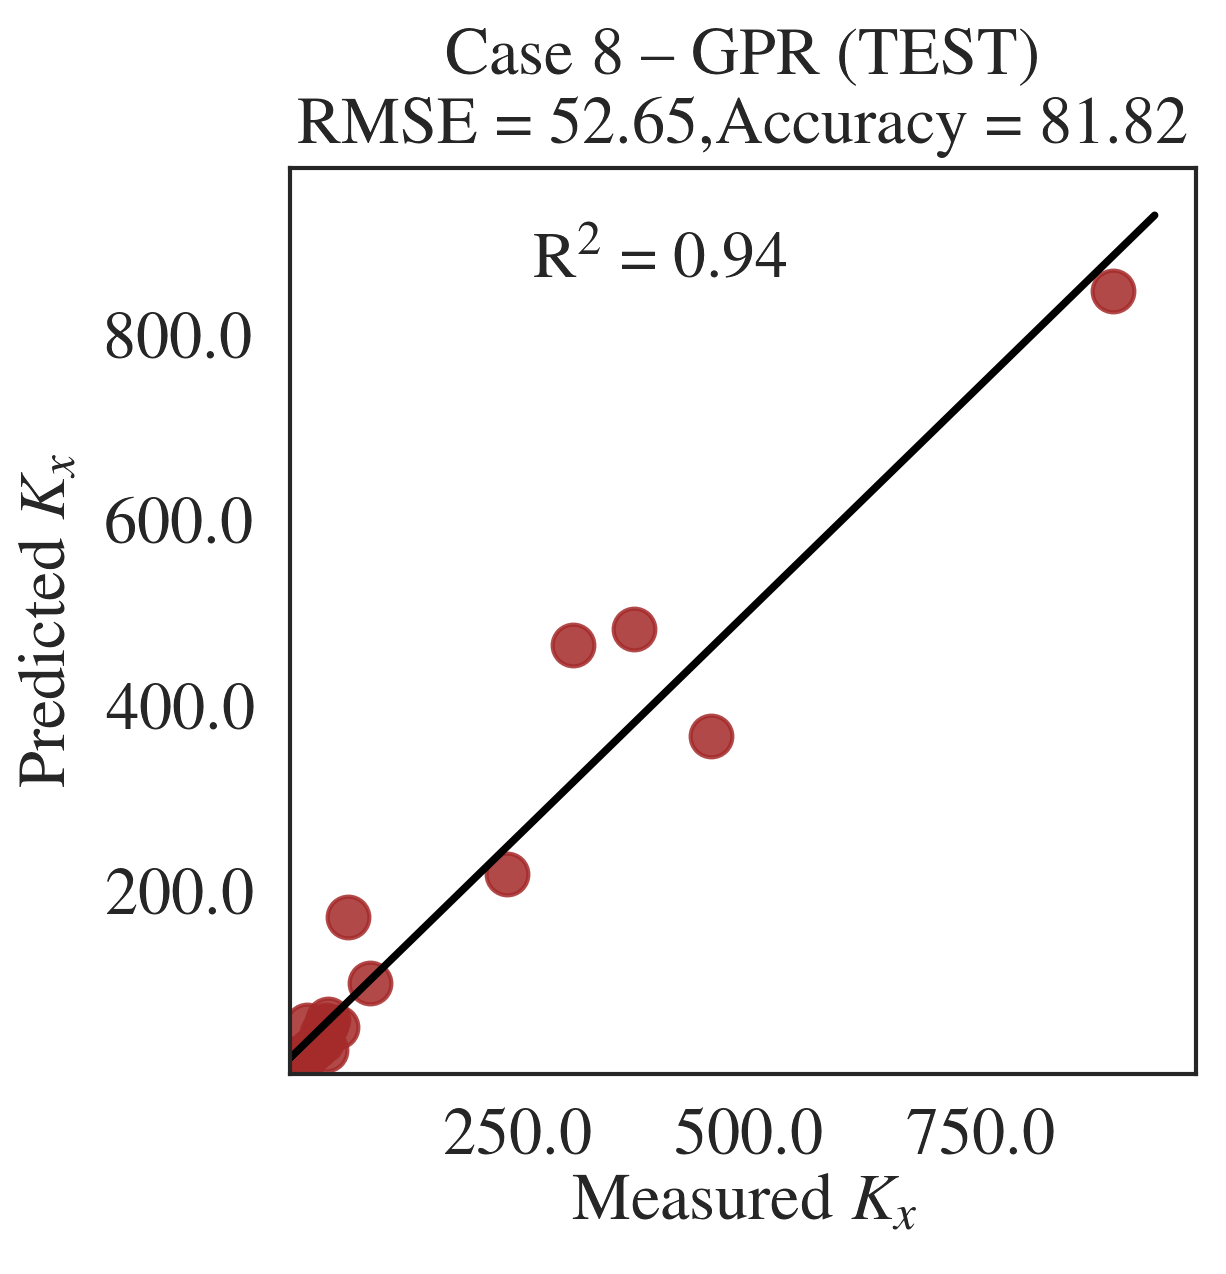
\includegraphics[width=0.33245\textwidth]{./scatter/eml____300dpi_scatter_best_model___gpr__case_8__test}
 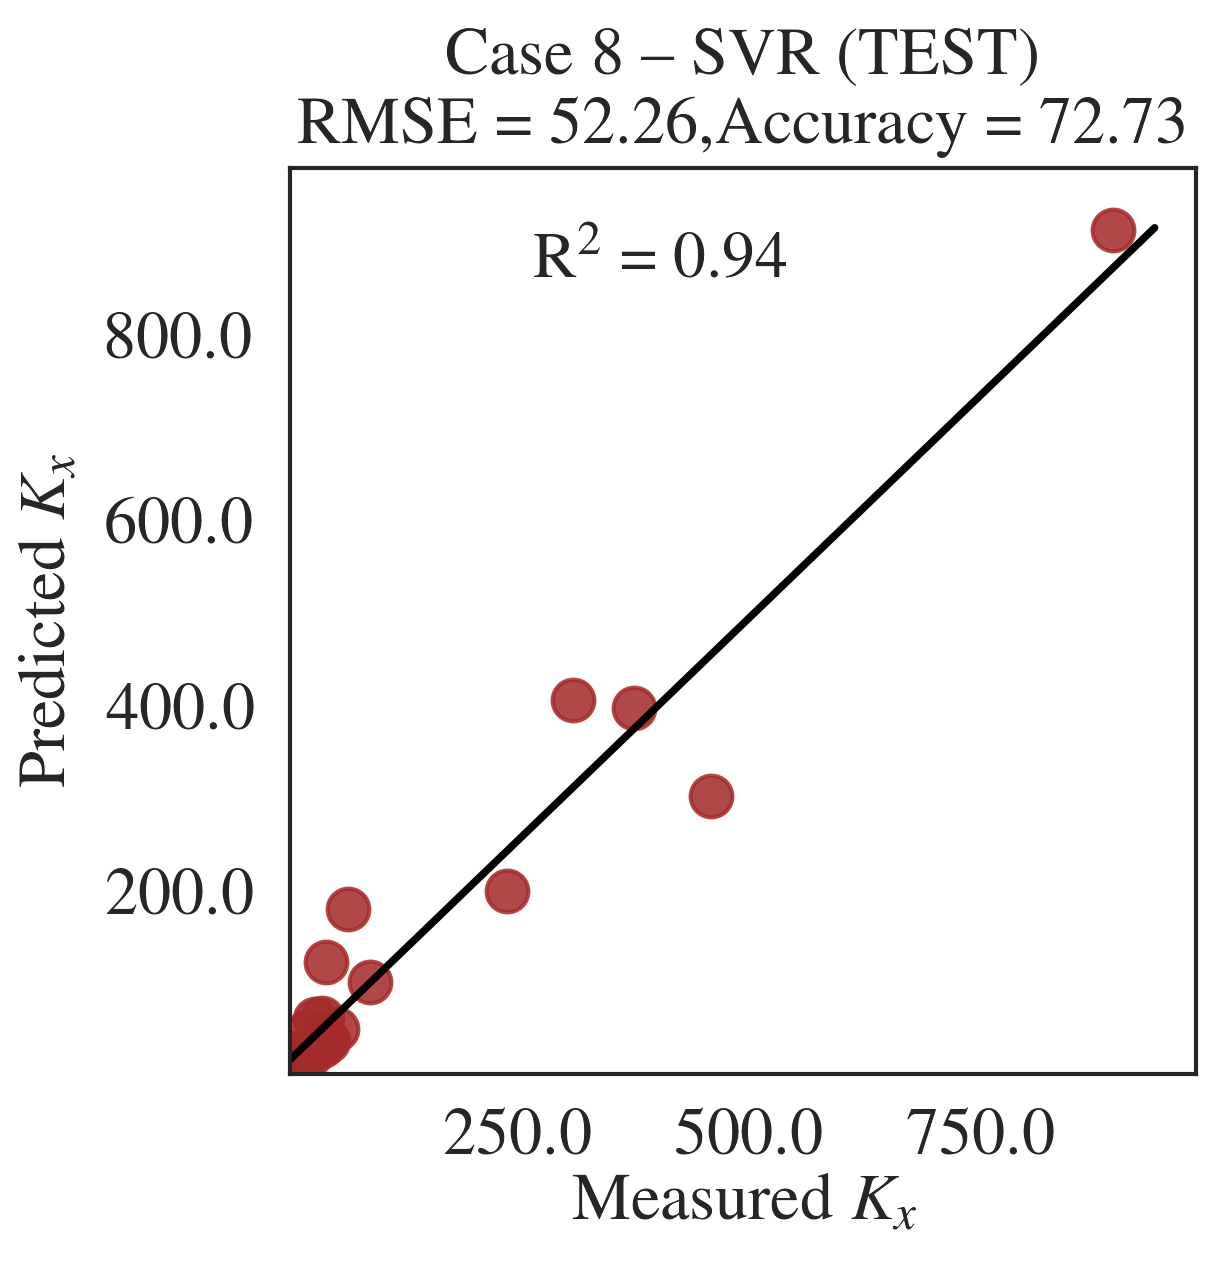
\includegraphics[width=0.33245\textwidth]{./scatter/eml____300dpi_scatter_best_model___svr__case_8__test}
 \caption{\label{fig:eml____300dpi_scatter_best_model_new___ldc}
 Scatter plots for the best models in Case 8 according to Root Mean Squared Error.}
\end{figure}


Further research includes multiobjective feature selection \cite{jimenez:2017}.

% Very few studies have recognized the the role of the channel sinuosity to estimate the dispersion coefficient.

% The definition of the sinuosity, defined by the the ratio between the channel length and the valley length, affects considerably the dispersion coeficcient. 

Some studies show that other exogenous factors may affect the sinuosity, such as vegetation \cite{camporeale:2010, savickis:2016} and topography \cite{timar:2003, dijk2013sinuosity}.


% Some studies showed that inclusion of sinuosity as an input variable  improves significantly the performance of a neural network model \cite{sahay2011prediction}.



%---------------------------------------------------------------------------------
\section{\label{sec:conclusions} Conclusions}
%---------------------------------------------------------------------------------
The dispersion of pollutants in rivers involves complex phenomena, requiring simplifications and assumptions, leading to drawbacks to accurate predictions. In this context, machine learning methods arise as an interesting alternative to dispersion coefficient modeling. However, the performance of these methods depends on the proper choice of the input variables.

In this paper, we have applied a machine learning pipeline that embeds a simple approach to the task of feature selection of dispersion coefficient of natural channels. 
The task of adjusting selected features and adjusting the parameters is assisted by an evolution strategy.
% 
Based on several studies on the literature, there is no attempt to integrate the feature selection to the model building step for predicting the dispersion coefficient. 
In general the feature selection task is performed in a separated step, and doe not considers the estimation model. 

The model proposed in this paper automatically searches for the features and the internal parameters of the machine learning models.
% 
The performance of the models was measured based on the root mean squared error and accuracy.
The results show that by the selection of the most suitable features, more efficient models for dispersion coefficient can be constructed. 
    




\bibliographystyle{unsrt}
\bibliography{references}

\end{document}
